% basically this is a template file, you should be able to take it and
% start running.

% the philosophy behind this template is that each chapter or
% chapterlike section goes in a separate file and you use the \include
% command to input it into the final document.  The \includeonly
% command can be used so you only need to work on one or two chapters at a
% time (instead of having to either latex the entire book each time or
% losing cross-references and page numbering)

% copy this file and call it something like mythesis.tex

%\documentclass[12pt]{report}
%\documentclass[oneside,10pt,final]{report}
\documentclass[twoside,10pt,final]{report}
%\documentclass[twoside,10pt,draft]{report}
% note that the documentclass can take other option such as
% twoside - for double sided printing
% openright - if double side  chapters always start on odd pages
% openany - if double side chapters start on the next page even or odd
% 12pt can be replaced by 11pt

\usepackage{suthesis-2e}
\usepackage{graphicx}
\usepackage{graphics}
\usepackage{amsmath}
\usepackage{amsthm}
\usepackage{amsfonts}
\usepackage{setspace}
%\usepackage{vmargin}


%\setpapersize{USletter}
%\setmarginsrb{1.6in}{0.7in}{1.1in}{0.6in}
%             {0.2in}{0.2in}{0.2in}{0.5in}

\setstretch{1.213}

\graphicspath{{../paper_topopt/figures/}
              {../paper_numcutoff/figures/}
              {../paper_symdyn/figures/}
             }

%%%%%%%%%%%%%%%%%%%%%%%%%%%%%%%%%%%%%
\DeclareMathOperator{\erf}{erf}
\DeclareMathOperator{\prob}{\mathbf{Prob}}
%%%%%%%%%%%%%%%%%%%%%%%%%%%%%%%%%%%%%
\newtheorem{assumption}{Assumption}
\newtheorem{definition}{Definition}
\newtheorem{theorem}{Theorem}
\newtheorem{lemma}{Lemma}
\newtheorem{example_base}{Example}
\newenvironment{example}{\begin{example_base}}
   {\hspace{\stretch{1}}$\lozenge$\end{example_base}}


\newcommand{\todo}[1]{\vspace{5 mm}\par \noindent
\marginpar{\textsc{Todo}}
\framebox{\begin{minipage}[c]{0.90 \textwidth}
\tt \flushleft #1 \end{minipage}}\vspace{5 mm}\par}

\renewcommand{\todo}[1]{}


\newcommand{\clearemptydoublepage}
 {\newpage{\thispagestyle{plain}\cleardoublepage}}



%% uncomment the following and create mythesis-macros.sty for all your
%% own macros.  This keeps this top level file looking fairly neat.
% \usepackage{mythesis-macros}

%% certain types of theses require special title page format.  See the
%% style file for the full list.  An example would be that for some of
%% the language departments. 
% \dualthesis \dept{Asian Languages} \languagemajor{Korean} 
%% or education
% \educationthesis

%\includeonly{../paper_numcutoff/paper_numcutoff_body,../paper_numcutoff/paper_topopt_body}



\begin{document}

    \title{Cutoffs in Chaotic Map Mixing and Topology Optimization of Microfluidic Channels}
    \author{Tzu-Chen Liang}
    \dept{\\Aeronautics and Astronautics} 
    \principaladviser{Matthew West}
    \firstreader{Sanjay Lall}
    \secondreader{Michael Saunders}
    \submitdate{March 2008}
    \tablespagefalse
    
    
    \beforepreface
    \prefacesection{Preface}
     %
% Preface
%
% This is the same as the abstract

This thesis studies chaotic mixing induced by microfluidic channels and builds the relation between it and the cutoff phenomenon in finite Markov Chains. We develop a topology optimization methodology for optimizing the shape of pressure-driven microfluidic channels to maximize the passive mixing rate of advected tracers. The optimization procedure uses a relaxation of Stokes flow by allowing a permeable structure, and the objective can be a function of either the fluid velocity field or the particle map from inlet to outlet. We present two new channel
designs, one that is an optimized version of the herringbone mixer of Stroock et al., and one that mixes more quickly by using a fully 3-D structure in the channel center. These channels deliver approximately 30\% and 60\% reductions in the 90\% mixing lengths. To compare our numerical simulations to experiments we approximate the inlet-outlet particle map by a Markov Chain and show that this cheaply approximates the true stochastic map.

We then numerically study the decay of the variance of a passive scalar function advected by the Standard Map when the diffusion goes to zero. The Markov Chain model we developed for microfluidic mixing channel simulation is applied here with very high resolution (up to $6.4 \times 10^9$ states) to approximate near-zero diffusion. Our numerical evidence shows that the mixing trajectories of the Standard Map can be characterized by using the cutoff phenomenon for finite Markov Chains.

In the last part of this thesis, we apply the definition of the cutoff phenomenon to the study of the evolution of a probability density function by 1-D chaotic maps. A new object called a stochastic symbol sequence is developed to prove that for a set of initial distributions, the total variation versus iteration curves present cutoffs. Moreover, we can generate a set of initial probability distributions such that when evolved by chaotic maps, they present the same limit behavior as the cutoff sequences found in specific finite Markov Chains. The results can be applied to any 1-D chaotic map that has full symbolic dynamics.



    \newpage


    \prefacesection{Acknowledgements}
      %
% acknowledgement
%
I am sincerely grateful to my research advisor Matthew West for his guidance and constant support. He is always there to share his experience and help me to clarify my thoughts. I enjoy every moment of our discussion. 
I thank Sanjay Lall for giving me the first opportunity of doing research at Stanford University, which deeply affects the direction of this thesis. I also wish to thank Michael Saunders for his precious comments for my thesis. 

I thank my friends and colleagues in the Department of Aeronautics and Astronautics for their help in my defense preparation and the great lunch-times we had.

Finally, I want to share my immense appreciation for the support and encouragement from my family, and their endless love throughout this entire journey.


    \afterpreface


 






% now for the body of the thesis, modify the number of these lines as needed

% this includes chapter1.tex which should start with a \chapter{...}
% command 

%%%%%%%%%%%%%%%%%%%%%%%%%%%%%%%%%%%%%%%%%%%%%%%%%%%%%%%%%%
%%%%%%%%%%%%%%%%%%%%%%%%%%%%%%%%%%%%%%%%%%%%%%%%%%%%%%%%%%
\chapter{Introduction}
%
% Thesis Introduction
%
%

\todo{TC: the paragraphs are from introductions of each papers}

This thesis deal with three topics in chaotic map mixing: the design and optimization of microfluidic mixing channels, the mixing trajectories of a scalar function advected by a chaotic map with near-zero diffusion, and the relation between chaotic map mixing and cutoff phenomenon. In this chapter we briefly review the current developments in each of these fields and introduce our approaches.  

  

%%%%%%%%%%%%%%%%%%%%%%%%%%%%%%%%%%%%%%
\section{Microfluidic mixing channels}
%%%%%%%%%%%%%%%%%%%%%%%%%%%%%%%%%%%%%%
Microfluidic systems control and manipulate liquids in microliter or nanoliter amounts. The study of microfluidics emerged in the 1990s and
is now widely applied in various fields such as the development of DNA chips \cite{Burns1998}, molecular biology \cite{DavidJ2002},
chemical reactions \cite{Andersson2000}, transfers of small volumes of materials \cite{Sammarco1999}, and lab-on-a-chip technology
\cite{weigl2003,Stone2004}. One of the challenges in microfluidics is the design of mixing channels, whose objective is to thoroughly mix
two or more different liquids. Although the mixers designed by using active components like micro-pumps to stir the flow have very
promising results \cite{Yang2000,Deshmukh2000}, passive mixing devices have advantages in manufacturing simplicity and price.

In chapter 2, we focus on the design and optimization of passive microfluidic mixing channels. A microfluidic mixing channel typically has
cross-section dimension $\ell\sim 100\nu m$, and the Reynolds number $\text{Re}=U\ell/\nu$ is less than $100$ \cite{Stroock2002} ($U$ is the average
velocity of the liquid and $\nu$ is the kinematic viscosity of the fluid).  Fluid flow on this scale is highly laminar and the mixing of
materials between streams is purely diffusive. The dimensionless number that controls the length of the channel required for mixing is the
P\'{e}clet number ($\text{Pe}= U\ell/D$, where $D$ is the molecular diffusivity). For a pressure-driven mixing channel the mixing length can be
expected to grow linearly with $\text{Pe}$ and is usually much more than $1\,\text{cm}$. Hence various designs are proposed to stir the
flow inside the channel and produce transverse velocities to enhance the mixing \cite{Stroock2002, Ottino2004Science, Wiggins2004}.

The mixing problem has been linked to chaotic mixing protocols, which
are believed to have the best mixing results because of the stretching and
folding features of chaotic maps. A typical way to realize chaotic
mixing is through the design of linked twist maps, and has been
studied in \cite{Wiggins2004}. However, there is no direct way to
realize the designed linked twist map in a mixing channel, either by
passive structure or by active mechanisms such as variable-frequency
pumps or internal moving components. We use the
techniques developed in topology optimization to find the internal
structure of a mixing channel to realize a desired flow field or flow
map. The results can be applied to mixing channel design when the
desired mixing protocol is known.

%%%%%%%%%%%%%%%%%%%%%%%%%%%%%%%%%%
\section{Topology optimization}
%%%%%%%%%%%%%%%%%%%%%%%%%%%%%%%%%%
A typical topology optimization problem is to distribute a given amount of material in a design domain subject to load and support
conditions such that the stiffness of the structure is maximized \cite{Bendsoe2003}. The design parameters are usually the spatial
distribution of the material. Even though the optimal solution is in general quite sparse in space, the number of variables is often
inevitably large in the formulation. Some problems, such as truss topology design, can be formulated as a convex optimization
problems \cite{BenTal1997} by relaxing the material density to be progressive and solved by efficient algorithms. The optimal solution of
the relaxed optimization is shown to be a black/white solution and thus also the optimal solution of the original problem. In other cases
when the problem has no convex formulation, nonlinear optimization techniques need to be applied and it is in general hard.


Topology optimization has been applied to the design of optimal shapes
of pipes or diffusers such that the total potential power drop is
minimized \cite{Evgrafov2005, Borrvall2003}. Darcey flow is used to
simulate the flow inside porous material and form a relaxation. The
design parameters in this formulation are the permeability of the
material on a spatial grid. In this case, the relaxed problem is still
non-convex, but can be solved by means of sequential separable and
convex programming. A two-step solution procedure is thus applied to
find a black/white solution with permeability either $0$ or infinity
at a point.

In this thesis we use the same relaxation strategy to formulate the
mixing channel design as a topology optimization problem. The
objective function we use is a function of the velocity field or a map
between the inlet and the outlet of one period of the channel. It is a
nonlinear optimization problem, and a sub-gradient method is developed
to find a local minimum of the objective function. We do not
consider the fabrication issue explicitly when solving the topology
optimization problem.


%%%%%%%%%%%%%%%%%%%%%%%%%%%%%%%%%%%%%%%%%%%%%%%%%%%%%%%%%
%%%%%%%%%%%%%%%%%%%%%%%%%%%%%%%%%%%%%%%%%%%%%%%%%%%%%%%%%
\section{The simulation of Advection-Diffusion equation}
%%%%%%%%%%%%%%%%%%%%%%%%%%%%%%%%%%%%%%%%%%%%%%%%%%%%%%%%%
%%%%%%%%%%%%%%%%%%%%%%%%%%%%%%%%%%%%%%%%%%%%%%%%%%%%%%%%%
Another challenge in the design of microfluidic mixing channels is
that there is no clear measure of how well a channel mixes. In
experiments it is common to measure the variance of colored liquids on
the cross-section of the channel to see how well they are mixed
\cite{Stroock2002}. However, when doing simulation, this corresponds
to solving the Advection-Diffusion equation for a 3-D flow field, which
is expensive. The problem that there is no clear link between the
variance of the liquid on a cross-section and the channel structures
remains hard so far. In this thesis, we develop a Markov Chain model to
approximate the mixing process.  Similar approaches can be found in,
for example, \cite{Dellnitz1999, Dellnitz2002, Froyland1998,
Froyland1999, Froyland2001}. It is a cheap way to replace the solving
of Advection-Diffusion equation and can let one observe the mixing
process and measure the variance of the colored field easily. This
model is by no means an accurate solution of the Advection-Diffusion
equation, but it captures the most important factors of the chaotic
mixing: stretching, folding, and molecular diffusion.




%%%%%%%%%%%%%%%%%%%%%%%%%%%%%%%%%%%%%%%%%%%%%%%%%%%%%%%%%%%%%%%%%%%%%%%%%%%
%%%%%%%%%%%%%%%%%%%%%%%%%%%%%%%%%%%%%%%%%%%%%%%%%%%%%%%%%%%%%%
\section{The multi-stage feature of chaotic mixing processes}
%%%%%%%%%%%%%%%%%%%%%%%%%%%%%%%%%%%%%%%%%%%%%%%%%%%%%%%%%%%%%%

% 
The question of how chaotic advection mixes a passive scalar function
has attracted much research effort in recent years
\cite{Ottino2004}. The main issues in this field are: how to measure
the thoroughness of the mixing, how the mixing process changes
qualitatively and quantitatively when the diffusion is close to zero,
and how to enhance the overall mixing process by designing the map
that produces chaotic advection. Unfortunately, we have only partial
understanding for most of these topics. In spite of the fact that the
detailed mechanism of mixing is unclear, non-trivial mixing processes
have been observed in experiments \cite{Rothstein1999, Voth2002} and
can be simulated by large-scale computations \cite{topopt,
  Tsang2005}. 
In chapter 3, we use the Markov Chain model we built for the simulation of microfludic mixing channels to simulate the chaotic mixing with small diffusion. Similar approaches for nonlinear dynamical systems can be found in, for example,
\cite{Dellnitz1999, Dellnitz2002, Froyland1998, Froyland1999,
  Froyland2001}. This simple and parallelizable linear model not only
captures the multi-stage feature of a chaotic mixing process, but also
generates a series of finite Markov Chains through which we can
observe the multi-stage feature of the mixing trajectory near the
zero-diffusion limit.



A widely observed phenomenon in the chaotic mixing process when small
diffusion exists is the two- or three-stage transition
\cite{Thiffeault2003-13, Fereday2002, Antonsen1996, Mezic2005}. The
map does not mix the scalar function with a constant rate in
general. When the variance of the scalar function is measured during
the mixing process, one can in general observe a relatively flat decay
initially, followed by a super-exponential change, and then finally it
tends to a exponential decay. We are interested in when these
transitions happen, why they happen, and how to predict the slope of
the exponential region. A good review and physical interpretation can
be found in \cite{Thiffeault2004}.

Thiffeault and Childress \cite{Thiffeault2003-13} study these
properties for a modified Arnold's cat map. Analytical formulas are
given to predict the transitions as well as the slopes. Because the
linear part of this map has an eigenvalue 2.618, which stretches very fast, 
and the chaotic part is relatively small, the three phases are
separated clearly. The same analytical procedure cannot be applied to,
for example, the Standard Map, although the only difference between the
Standard Map and the modified Arnold's cat map is in the linear part.

\todo{MW: Check rewording of sentence in above paragraph starting
  ``Because the linear part \ldots''}

As for the exponential decay part, there is still debate about whether
the decay rate goes to zero in the zero diffusivity limit or whether
it tends to a constant independent of the diffusion
\cite{Thiffeault2004, Tsang2005}. Theoretical analysis shows that both of
these possibilities can occur for different chaotic flows
\cite{Haynes2005}.

Difficulties typically arise in studying the above problems
numerically, because the small diffusion usually means that fine grids are
required in the solution of the Advection-Diffusion equation or the
simulation of the map. Some studies and numerical results conclude that a
proportional relation exists between the stationary decay rate and the
diffusion \cite{Cerbelli2003, Pikovsky2003}. However, this is only true for
certain diffusion ranges.  


In \cite{Tsang2005}, the author
uses a simple and parallelizable numerical strategy that can simulate
up to $6 \times 10^4$ by $6 \times 10^4$ grids to show that the decay rate
of a certain chaotic map tends to a constant. However, general
numerical results for most other chaotic maps have not been found so
far.
  

In chapter 3 we focus on the mixing process of the Standard Map in
the near-zero diffusion limit. We present a numerical strategy to
simulate the map with very high resolution (up to $8 \times 10^4$ by
$8 \times 10^4$ grids) and hence very low numerical diffusion. This
numerical strategy is realized by a Markov Chain simulation. To
characterize the evolution of the scalar variance in the near-zero
diffusion limit, we use the concept of cutoff from the study of finite
Markov Chains. We present numerical evidence to suggest that the
sequence of models presents a cutoff, which qualitatively
characterizes the mixing process when the diffusion goes to zero. The
main contribution of this paper is to build a bridge between finite
Markov Chain theory and $2$-D chaotic maps with small
diffusion. Related analytical results for $1$-D chaotic maps
clarifying their relationship to the cutoff phenomenon can be found in
\cite{symdyn}.







%%%%%%%%%%%%%%%%%%%%%%%%%%%%%%%%%%%%%%%%%%%%%%%%%%%%%%%%%%%%%%%%%%%%%%%%%%%%

%%%%%%%%%%%%%%%%%%%%%%%%%%%%%%%%%%%%%%%%%%%%%%%%%%%%%%%%%
\section{Cutoff phenomenon and symbolic dynamics}
%%%%%%%%%%%%%%%%%%%%%%%%%%%%%%%%%%%%%%%%%%%%%%%%%%%%%%%%%
How many riffle shuffles are required to sufficiently mix 52 cards? This question have been
answered by Bayer and Diaconis in \cite{Diaconis1992}. It is quite surprising that the cards are
highly ordered in the first several shuffles (6 for 52 cards) and then randomized almost abruptly.
This kind of sharp change in some measure of order/disorder has been discovered in many finite
Markov Chains, and named cutoff phenomenon \cite{Diaconis1986}. A recent review about the cutoff
phenomenon of random walks on finite groups can be found in \cite{LSaloff-Costt2004}. On the other
hand, chaotic mixing process is observed to have similar
properties \cite{Thiffeault2003-13, Thiffeault2004, Tsang2005}. Think of the cream poured
into coffee, while stirring, the cream keeps stretching for a while and the mixing with coffee
happens suddenly. Chaotic mixing has been applied in, for example, microfluidic mixing channel
design \cite{Ottino2004Science, Wiggins2004, Ottino2004}, random search strategies and
generating random numbers. However, it is still unclear how to characterize and measure the mixing
process. In chapter 4, we try to build the relation between cutoff phenomenon and the chaotic
mixing process by generalizing symbolic dynamics of chaotic maps. The result shows ``cutoff'' in
the mixing process can be produced by chaotic maps with full symbolic dynamics and certain initial
conditions.



%%%%%%%%%%%%%%%%%%%%%%%%%%%%%%%%%%%%%%%%%%%%%%%%%%%%%%%%%%
%%%%%%%%%%%%%%%%%%%%%%%%%%%%%%%%%%%%%%%%%%%%%%%%%%%%%%%%%%
\chapter{Optimized Mixing in Microfluidic Channels}
%
% Introduction of Chapter topopt 
%


We develop a topology optimization methodology for optimizing the
shape pressure-driven microfluidic channels to maximize the passive
mixing rate of advected tracers. The optimization procedure uses a
relaxation of Stokes flow by allowing a permeable structure and the
objective can be a function of either the fluid velocity field or the
particle map from inlet to outlet. We present two new channel designs:
one that is an optimized version of the herringbone mixer of Stroock
et al., and one that mixes more quickly by using a fully 3D structure
in the channel center. These channels deliver approximately 30\% and
60\% reductions in the 90\% mixing lengths. To compare our numerical
simulations to experiments we approximate the inlet-outlet particle
map by a Markov Chain and show that this cheaply approximates the true
stochastic map.

%In this chapter, we focus on the design and optimization of passive microfluidic mixing channels. A microfluidic mixing channel typically has
%cross-section dimension $ell\sim 100\mu m$, and Reynolds number $\text{Re}=U\ell/\nu$ is less than $100$ \cite{Stroock2002} ($U$ is the average
%velocity of the liquid and $\nu$ is the kinematic viscosity of the fluid).  Fluid flow on this scale is highly laminar and the mixing of
%materials between streams is purely diffusive. The dimensionless number that controls the length of the channel required for mixing is
%P\'{e}clet number ($\text{Pe}= U\ell/D$ where $D$ is the molecular diffusivity). For a pressure-driven mixing channel the mixing length can be
%expected to grow linearly with $\text{Pe}$ and is usually much more than $1\,\text{cm}$. Hence various designs are proposed to stir the
%flow inside the channel and produce transverse velocities to enhance the mixing \cite{Stroock2002, Ottino2004Science, Wiggins2004}.

%The mixing problem has been linked to chaotic mixing protocols, which
%are believed to have the best mixing results due to the stretching and
%folding features of chaotic maps. A typical way to realize chaotic
%mixing is through the design of linked twist maps, and has been
%studied in \cite{Wiggins2004}. However, there is no direct way to
%realize the designed linked twist map in a mixing channel, either by
%passive structure or active mechanisms such as variable-frequency
%pumps or internal moving components. In this paper, we use the
%techniques developed in topology optimization to find the internal
%structure of a mixing channel to realize a desired flow field or flow
%map. The results can be applied to mixing channel design when the
%desired mixing protocol is known.


%Topology optimization has been applied to the design of optimal shapes
%of pipes or diffusers such that the total potential power drop is
%minimized \cite{Evgrafov2005, Borrvall2003}. Darcey flow is used to
%simulate the flow inside porous material and form a relaxation. The
%design parameters in this formulation are the permeability of the
%material on a spatial grid. In this case, the relaxed problem is still
%non-convex, but can be solved by means of sequential separable and
%convex programming. A two-step solution procedure is thus applied to
%find a black/white solution with permeability either $0$ or infinity
%at a point .

%In this chapter we use the same relaxation strategy to formulate the
%mixing channel design as a topology optimization problem. The
%objective function we use is a function of the velocity field or a map
%between the inlet and the outlet of one period of the channel. It is a
%nonlinear optimization problem and a sub-gradient method is developed
%to find the local minimum of the objective function. We do not
%consider the fabrication issue explicitly when solving the topology
%optimization problem.

In section \ref{sec:opt} we describe the mathematical model of mixing
channels and how to form the topology optimization problem using a
relaxation of Stokes flow. Section \ref{sec:simu} discusses the
simulation issue, and a Markov chain model is proposed to approximate
the solution of the advection-diffusion equation to evolve the color
intensity field. Results are given in section \ref{sec:topoptresults} and 
conclusions are in section \ref{sec:topoptconclusion}.

%
% Body
%
%%%%%%%%%%%%%%%%%%%%%%%%%%%%%%%%%%%%%%%%%%%%%%
%%%%%%%%%%%%%%%%%%%%%%%%%%%%%%%%%%%%%%%%%%%%%%
\section{Forming the optimization problem}
\label{sec:opt}
%%%%%%%%%%%%%%%%%%%%%%%%%%%%%%%%%%%%%%%%%%%%%%
%%%%%%%%%%%%%%%%%%%%%%%%%%%%%%%%%%%%%%%%%%%%%%

%%%%%%%%%%%%%%%%%%%%%%%%%%%%%%%%%%%%%%%%%%%%%%
\subsection{Mathematical model of a periodic microfluidic mixing channel}
%%%%%%%%%%%%%%%%%%%%%%%%%%%%%%%%%%%%%%%%%%%%%%


We are concerned with mixing in a thin and long channel. Fluids with
two different colors (with intensities $1$ and $0$) are injected in
one end of the channel and flow through it driven by body force
only. The channel has some internal structure that acts to stir the
fluid passively. This structure is periodic with period $\ell_x$ and the
cross-section of the channel has dimension $\ell_y$ by $\ell_z$. The channel
is assumed to be long enough so that the velocity field inside is
fully developed and hence also periodic with period $\ell_x$. Because of the
periodic velocity field, we need to solve it for only one period, and
we can then use this velocity field to transport the fluid with
different colors iteratively to observe the mixing process. In fact,
we calculate the streamlines that connect the two ends ($x=0$ and
$x=\ell_x$) of one period length channel and define a Poincar\'e
map. Applying this map repeatedly tells us how a particle moves
between different cross-sections along the channel.



\begin{figure}
  \centerline{
    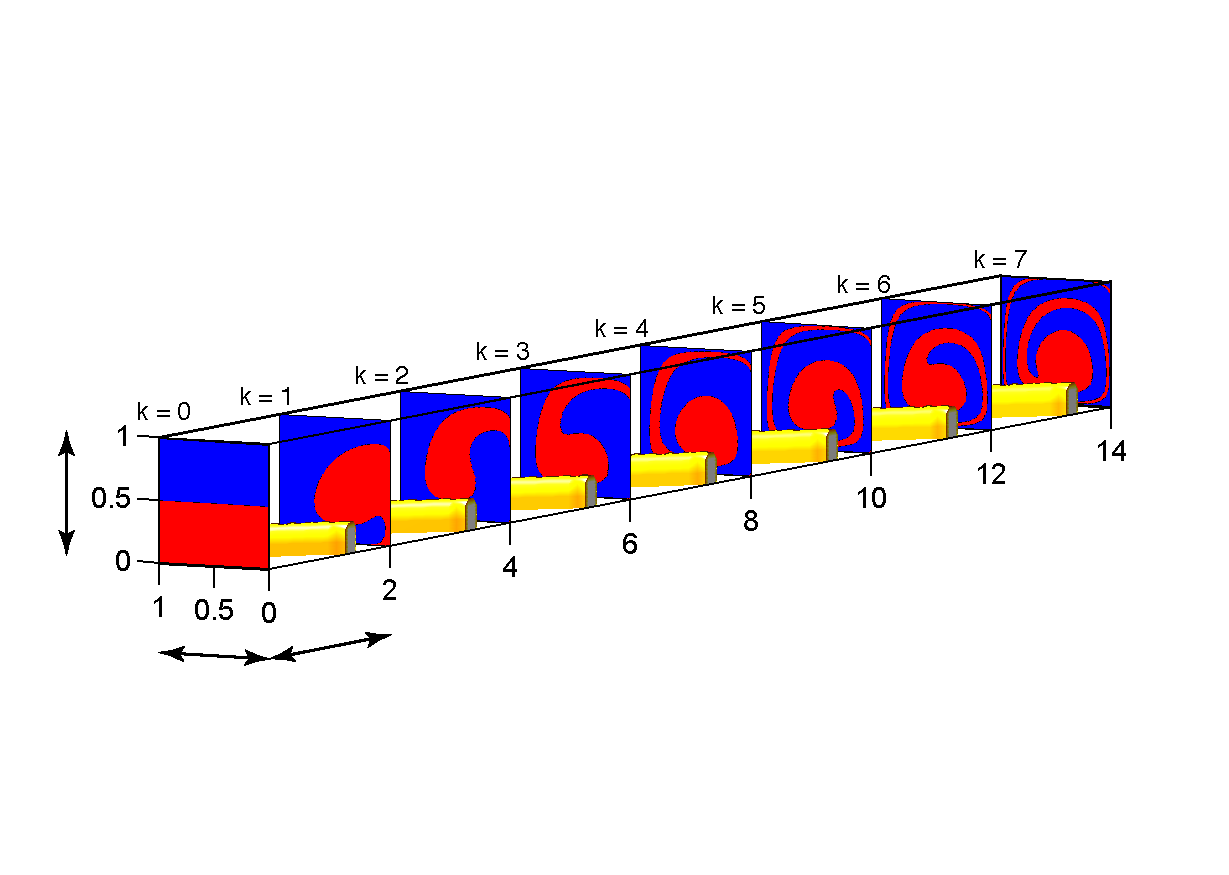
\includegraphics[width=0.8\textwidth,trim=0cm 3cm 0cm 2cm,clip]{mixingchannel}}
  \caption{\label{mixingchannel} The mixing channel. Liquids with two
    different colors are originally separated and injected from one
    side of the channel. Inside the channel there are periodic
    structures to stir the flow and produce transverse velocity
    components. The colored liquids then start to mix. In this figure,
    cross-sections of the color distribution are plotted every period
    of the structure.}
\end{figure}


As mentioned in the introduction, flow on the microfluidic
scale has $\text{Re}\sim 1$ and is thus highly laminar. A Stokes partial
differential equation is generally a reasonable model of the motion.
We simulate the flow by the generalized Stokes equation for
incompressible flow:
\begin{subequations}
  \label{stokes}
  \begin{align}
    \label{stokes1}
    ( -\nu\Delta + \alpha)u
    + \nabla p &= f, \\
    \label{stokes2}
    \mbox{div} u &= 0,
  \end{align}
\end{subequations}
where $u(\mathbf{x})$ and $p(\mathbf{x})$, which are both functions of
position $\mathbf{x}=(x,y,z)$, stand for the velocity and pressure
fields and $f$ is the body force that drives the flow. It has an
elliptic operator $-\nu\Delta + \alpha $ in which $\nu$ is the
kinematic viscosity and $\alpha(\mathbf{x})$ represents the inverse
permeability at $\mathbf{x}$. When $\alpha(\mathbf{x}) = 0 $ it is
just Stokes flow with viscosity $\nu$ and when $\nu=0$, one gets the
Darcy equation, which governs the flow in porous material with
permeability $\alpha^{-1}$. The liquids to be mixed are assumed to
have the same density and viscosity, which is true for
many applications when the liquids are solvents carrying different
reactants. This assumption is critical for our periodic setting 
to work, because now we can separate the color intensity field from 
the velocity field: the velocity field is stationary but the color 
intensity field has not. This allows us to use one period of velocity 
field repeatedly to carry the color intensity and observe the mixing process. 

 

\todo{MW: When I gave the talk on this last week there were a number
  of people confused because they thought that $\alpha$ was a scalar,
  rather than a scalar function of position. I think it might be worth
  making it clear that we have $u(x)$, $p(x)$ and $\alpha(x)$.}
\todo{TC: We use $x$ as one coordinate, so $u(x)$ is also confusing.
So I think $u(\mathbf{x})$ is better, and define $\mathbf{x}=(x,y,z)
$}

\todo{MW: Thinking about it further, the assumption that they liquids
  have the same density and viscosity is actually critical for our
  whole method, isn't it? If the flow field depended on the color then
  we couldn't do a period solve at all, as the equation would keep
  changing as we went further down the channel and the mixing state
  changed. So it's not just for simplicity that we assume that, but
  rather we really need to assume it. We should make this clear.}

\todo{TC:Agree. A sentence is added in above.}

We use a finite-difference method with staggered regular meshes to
solve the above equation. Assuming the finite-dimensional
approximation of the Laplace, gradient and divergence operators on the
given mesh are $L$, $G$, and $D$, the generalized Stokes equation can
be represented by
\begin{equation}
  \label{discretestokes}
  \left[\begin{matrix}
      -\nu L + \text{diag}(\bar{\alpha})H & G\\
             D                            &  0
    \end{matrix} \right]
  \left[\begin{matrix}
      \bar{u} \\ \bar{p}
    \end{matrix} \right]=
  \left[\begin{matrix}
      \bar{f} \\ \mathbf{0}
    \end{matrix} \right],
\end{equation}
where $\bar{u}$, $\bar{p}$, $\bar{\alpha}$, and $\bar{f}$ are vectors, representing
finite-dimensional approximations of $u$, $p$, $\alpha$ and $f$,
respectively. The linear operator $H$ maps the design parameters
$\bar{\alpha}$ to the directional $\bar{u}$ grids.



Let the number of grids in the $x$, $y$, and $z$ directions be $n_x$,
$n_y$, and $n_z$. We define $n_{\bar{u}} = 3n_x n_y n_z$, which is
roughly the size of $\bar{u}$, and $n_{\bar{\alpha}}=n_{\bar{p}} = n_x
n_y n_z$, which is roughly the size of $\bar{\alpha}$ and $\bar{p}$. A
typical case in our examples is $n_x = 144$, $n_y=24$, and $n_z=48$.



%%%%%%%%%%%%%%%%%%%%%%%%%%%%%%%%%%%%%%%%
\subsection{Topology optimization}
%%%%%%%%%%%%%%%%%%%%%%%%%%%%%%%%%%%%%%%%

We would like to optimize some objective function
$g(\bar{u},\bar{p},\bar{\alpha})$ over parameters $\bar{\alpha}$. The
direct approach would be to define an optimization problem
%\begin{align}
%\begin{split}
%  \text{minimize    } &
%  g(\bar{u},\bar{p},\bar{\alpha})\\
%  \text{subject to  } &\left[\begin{matrix} -\nu L + \text{diag} (\bar{\alpha}) H
%       & G \\ D & 0
%    \end{matrix} \right]
%    \left[\begin{matrix}
%      \bar{u} \\ \bar{p}
%    \end{matrix} \right]=
%    \left[\begin{matrix}
%     \bar{f} \\ \mathbf{0}
%    \end{matrix} \right], \\
%    &0 \le \bar{\alpha} \le \alpha_{\text{max}}
%    %& \mathbf{0}\le \bar{\alpha} \le \alpha_M\mathbf{1}
%\end{split}
%\end{align}
\begin{eqnarray}
\begin{array}{ll}
  \text{minimize}     & g(\bar{u},\bar{p},\bar{\alpha})\\
  \text{subject to  } &\left[\begin{matrix} -\nu L + \text{diag} (\bar{\alpha}) H
       & G \\ D & 0
    \end{matrix} \right]
    \left[\begin{matrix}
      \bar{u} \\ \bar{p}
    \end{matrix} \right]=
    \left[\begin{matrix}
     \bar{f} \\ \mathbf{0}
    \end{matrix} \right], \\
    &0 \le \bar{\alpha} \le \alpha_{\text{max}},
\end{array}
\end{eqnarray}
where $\alpha_{\text{max}}\in \mathbb{R}$ is a large number to approximate the minimum
permeability when $\alpha$ goes to infinity and the structure is
solid. The optimization problem has variables $\bar{u}$,
$\bar{p}$, and $\alpha_{\text{max}}$, and a large set of nonlinear equality
constraints that make the problem extremely hard to solve.

\todo{MW: I think that we can just say $0 \le \bar{\alpha} \le
  \alpha_{\text{max}}$ and say explicitly that $\alpha_{\text{max}}
  \in \mathbb{R}$. This notation is no more confusing that using $\le$
  on vectors in the first place, I think?}
\todo{TC: agree}

For a given $\bar{\alpha}$, we can solve \eqref{discretestokes} to
obtain $\bar{u}$ and $\bar{p}$ and there are no inequality constraints
on these two variables. We can thus rewrite the optimization and lump
the equality constraints into the objective function:
\begin{eqnarray}\label{topoptform}
  \begin{array}{ll}
    \text{minimize } & g(\bar{u}(\bar{\alpha}),
    \bar{p}(\bar{\alpha}), \bar{\alpha})
    \\ \text{subject to } & 0\le \bar{\alpha} \le \alpha_\text{max}.
  \end{array}
\end{eqnarray}
This formulation reduces the number of variables and eliminates the
nonlinear equalities, but it is now harder to evaluate the gradient of
the objective function, which we desire for efficiency in the
optimization algorithm. We will show later that an adjoint method can
be applied to efficiently compute the gradient.

%%%%%%%%%%%%%%%%%%%%%%%%%%%%%%%%%%%%%%%%%%%%%%%%%%%%%%%%
\subsection{Objective functions and a descent direction}
%%%%%%%%%%%%%%%%%%%%%%%%%%%%%%%%%%%%%%%%%%%%%%%%%%%%%%%%

%%%%%%%%%%%%%%%%%%%%%%%%%%%%%%%%%
\paragraph{Objective functions.}
%%%%%%%%%%%%%%%%%%%%%%%%%%%%%%%%%
Our goal is to optimize the shape of the structure inside the channel,
that is to find a vector $\bar{\alpha}$ such that the function
$g(\bar{u},\bar{p},\bar{\alpha})$ is locally minimized. The ideal
objective function is mixing length \cite{Stroock2002}: the channel
length required for the standard deviation of the color intensity on
the cross-section to drop by a given ratio. Unfortunately, this is a
very complicated function of the channel structure and there is no
clear way to find a descent direction to improve it. Hence, we use
several steps of heuristic designs to reduce the mixing length.

Two types of objective function will be considered in our
formulation. The first one is a function of the velocity field, which
is a very direct way to design the flow. In fact for most
applications, a linear function is good enough:
\begin{eqnarray}
  g_1(\bar{u},\bar{p},\bar{\alpha}) =
  \bar{c}^T\bar{u}.
\end{eqnarray}


\todo{MW: I don't like the notation below for $g_2$. Our $g$ objective
  functions should be functions of $u,p,\alpha$, not of
  $S_1,S_2$. Perhaps we can do something like define $S_u : [0,\ell_y]
  \times [0,\ell_z] \to [0,\ell_y] \times [0,\ell_z]$ to be the
  end-to-end particle map given by $u$, and then define
  $g_2(u,p,\alpha) = \|S^* - S_u\|$, or something like that?}

\todo{TC: fixed}

The second type of objective function
  measures the difference between two maps. Once the velocity is
  solved, the streamline can be calculated by numerical
  integration. Each of the streamlines connects a point on the $y$-$z$
  plane at $x=0$ to another point at $x=l_x$. The streamlines thus
  define an end-to-end flow map $S_u:[0,l_y]\times[0,l_z] \to
  [0,l_y]\times[0,l_z]$. Define $g_2(u,p,\alpha;S^*) = \|S^* - S_u\|$,
  where $S^*: [0,\ell_y] \times [0,\ell_z] \to [0,\ell_y] \times
  [0,\ell_z]$ is the desired end-to-end flow map and $\| \cdot \|$ is
  a distance measure of two maps $S_u$ and $S^*$. Suppose we know what
  the map we want is. The second type of objective function can then be
  applied to minimize the difference between the current map and the
  desired map. However, because each streamline needs to be calculated
  numerically, to define a map would be extremely hard. Therefore we
  simplify this objective function and let it measure the difference
  between a set of sample points on the $y$-$z$ plane. Let $(\bar{y}_0,\bar{z}_0)$
  be a set of sample points on the $y$-$z$ plane at $x=0$. We have
\begin{align*}
           (\bar{y}_e^*,\bar{z}_e^*)&= S^*(\bar{y}_0,\bar{z}_0), \\
           (\bar{y}_e,\bar{z}_e)    &= S_u(\bar{y}_0,\bar{z}_0). 
\end{align*}
We simply define $g_2$ as
\begin{eqnarray}
\label{g2}
           g_2(u,p,\alpha;S^*,\bar{y}_0,\bar{z}_0) = \|\bar{y}_e^*-\bar{y}_e\|^2 +  \|\bar{z}_e^*-\bar{z}_e\|^2,
\end{eqnarray}
where $\|\cdot\|$ is the $2$-norm of a vector. The above function is
a rough measure of how close the maps $S_u$ and $S^*$ are. In our
examples, $(\bar{y}_0,\bar{z}_0)$ is chosen as regular mesh grids on the $y$-$z$
plane.
%%%%%%%%%%%%%%%%%%%%%%%%%%%%%%%%%%%%%%%%%%%%%%%%%%%%%%%%%%%%%%%%%%%%
\paragraph{Adjoint method for $d g_1/d \mathbf{\bar{\alpha}} $.}
%%%%%%%%%%%%%%%%%%%%%%%%%%%%%%%%%%%%%%%%%%%%%%%%%%%%%%%%%%%%%%%%%%%%
To find a descent direction of $g_1$ with respect to $\bar{\alpha}$,
the adjoint method \cite{Jameson1999} is applied. Let $\bar{v} =
[\bar{u};\bar{p}]$. The variables $\bar{v}$ and $\bar{\alpha}$ satisfy
a set of constraints $R(\bar{v},\bar{\alpha})=0$, which is
stated in (\ref{discretestokes}). $d\bar{v}/d\bar{\alpha}$ has size
$(n_{\bar{u}}+n_{\bar{p}}) \times n_{\bar{\alpha}}$ (very large) and
is dense. We would like to calculate $d g_1/d\bar{\alpha}$ without
explicitly forming $d\bar{v}/d\bar{\alpha}$. The adjoint method is
designed for this situation. We begin with the total derivative of
$g_1$ and $R$ with respect to $\alpha$:
\begin{align*}
  \frac{dg_1}{d\bar{\alpha}} & =  \frac{\partial{g_1}}{\partial{\bar{\alpha}}}+
                                \frac{\partial{g_1}}{\partial{\bar{v}}} \frac{d\bar{v}}{d\bar{\alpha}},\\
  \frac{dR}{d\bar{\alpha}} & =  \frac{\partial{R}}{\partial{\bar{\alpha}}}+
                                 \frac{\partial{R}}{\partial{\bar{v}}} \frac{d\bar{v}}{d\bar{\alpha}}=0.
\end{align*}
From the second equation, we have
\begin{equation*}
  \frac{d\bar{v}}{d\bar{\alpha}}= -\left(\frac{\partial{R}}{\partial{\bar{v}}}\right)^{\dagger}\frac{\partial{R}}{\partial{\bar{\alpha}}}.
\end{equation*}
Substitute this into the first equation:
\begin{equation*}
   \frac{dg_1}{d\bar{\alpha}}  =  \frac{\partial{g_1}}{\partial{\bar{\alpha}}}-\frac{\partial{g_1}}{\partial{\bar{v}}} \left(\frac{\partial{R}}{\partial{\bar{v}}}\right)^{\dagger}\frac{\partial{R}}{\partial{\bar{\alpha}}}.
\end{equation*}
Let $\Phi = -\frac{\partial{g_1}}{\partial{\bar{v}}}
\left(\frac{\partial{R}}{\partial{\bar{v}}}\right)^{\dagger}$. Then
$\Phi$ satisfies
\begin{equation}
\label{adjointeq}
 \Phi \left(\frac{\partial{R}}{\partial{\bar{v}}}\right)^{T} = -\left({\frac{\partial{g_1}}{\partial{\bar{v}}}}\right)^T.
\end{equation}
The above equation is called the adjoint equation. More explicitly, the adjoint equation in our formulation is
\begin{equation}
\label{adjointeq2}
  \left[\begin{matrix}
     -\nu L + \text{diag}(\bar{\alpha})H   & G\\
     D               &  0
   \end{matrix} \right] \Phi^T =
  \left[\begin{matrix}
    -\frac{\partial{g_1}}{\partial{\bar{u}}}\\
    0
   \end{matrix} \right].
\end{equation}
After solving for $\Phi$, we can then evaluate $dg_1/d\bar{\alpha}$ by
\begin{equation}
\label{dg1dalpha}
  \frac{dg_1}{d\bar{\alpha}}  =  \frac{\partial{g_1}}{\partial{\bar{\alpha}}}+\Phi \frac{\partial{R}}{\partial{\bar{\alpha}}}.
\end{equation}
In our problem, $g_1$ does not depend on $\bar{\alpha}$ explicitly, so
the first term in the right-hand side of (\ref{dg1dalpha}) is zero. To
solve the adjoint equation (\ref{adjointeq2}), we need
$\partial{g_1}/\partial{\bar{u}}$, which is just $\bar{c}^T$ for
$g_1$.
%%%%%%%%%%%%%%%%%%%%%%%%%%%%%%%%%%%%%%%%%%%%%%%%%%%%%%%
\paragraph{Streamlines and $\partial g_2/\partial {\bar{u}}$.}
%%%%%%%%%%%%%%%%%%%%%%%%%%%%%%%%%%%%%%%%%%%%%%%%%%%%%%%
To find $d g_2/d \bar{\alpha}$, the above approach is still valid but
we need to form $\partial{g_2}/\partial{\bar{u}}$ first. Let the
solution of (\ref{discretestokes}) be the discrete velocity field
$\bar{u} = [\bar{u}_{x}; \bar{u}_{y}; \bar{u}_{z}]$. The velocity at
any point can be evaluated by linear interpolation. Given an initial
point $(0,y_{0},z_{0})$, a second-order Runge-Kutta method is applied to
find the streamline passing through it. Because both the interpolation
and Runge-Kutta method have linear weights on $\bar{u}$, we can write
down the following relations:
\begin{align*}
 x_e & =  k_{x}^T \bar{u}_{x}+0,\\
 y_e & =  k_{y}^T \bar{u}_{y}+y_{0},\\
 z_e & =  k_{z}^T \bar{u}_{z}+z_{0},
\end{align*}
where $k_{x},k_{y}$ and $k_{z}$ are the constant weighting vectors
generated by the numerical integration. $(x_e,y_e,z_e)$ is the point
where $(x_{0},y_{0},z_{0})$ maps to, assuming $x_e= \ell_x$.
$dy_e/d\bar{u}$ and $dz_e/d\bar{u}$ can be written as
\begin{align}
\begin{split}
 \frac{dy_e}{d\bar{u}} & =  \left[  \frac{\partial{y_e}}{\partial{x_e}} \frac{dx_e}{d\bar{u}_{x}},
                                        \frac{dy_e}{d\bar{u}_{y}},
                                        \mathbf{0}^T\right]
                                  =  \left[\frac{u_y(\mathbf{x}_e)}{(u_x(\mathbf{x}_e)}k_{x}^T,
                                        k_{y}^T ,\mathbf{0}^T    \right], \\
 \frac{dz_e}{d\bar{u}} & =  \left[  \frac{\partial{z_e}}{\partial{x_e}} \frac{dx_e}{d\bar{u}_{x}},
                                        \mathbf{0}^T,
                                        \frac{dz_{f}}{d\bar{u}_{z}}\right]
                                  = \left[\frac{u_z(\mathbf{x}_e)}{u_x(\mathbf{x}_e)_e}k_{x}^T,
                                        \mathbf{0}^T, k_{z}^T  \right],
\end{split}
\end{align}
where $\mathbf{x}_e= (x_e,y_e,z_e)$ and $u_x(\mathbf{x}_e),u_y(\mathbf{x}_e)$ and $u_z(\mathbf{x}_e)$ can also be evaluated by interpolation. Hence
$dg_2/d\bar{u}$, where $g_2$ has the form of equation (\ref{g2}), can
be written as
\begin{eqnarray}
   \frac{\partial g_2}{\partial \bar{u}} = \sum_{y_e} \frac{\partial{g_2}}{\partial{y_e}} \frac{dy_e}{d\bar{u}}+
                                    \sum_{z_e} \frac{\partial{g_2}}{\partial{z_e}}\frac{dz_e}{d\bar{u}}.
\end{eqnarray}
%%%%%%%%%%%%%%%%%%%%%%%%%%%%%%%%%%%%%%%%%%%%%%%%%%%%%%%%
\subsection{The gradient-based method}
%%%%%%%%%%%%%%%%%%%%%%%%%%%%%%%%%%%%%%%%%%%%%%%%%%%%%%%%
We use a gradient-based method to solve (\ref{topoptform}):

\begin{tabular}{ll}
\textbf{Algorithm} &\\
\hline
\textbf{given}  &    a starting vector $\bar{\alpha}^0$, $k=0$, $\star=1$ or $2$. \\
\textbf{repeat} &    1. solve (\ref{discretestokes}) for the velocity field.   \\
                &    2. solve the adjoint equation (\ref{adjointeq2}) and find $\frac{dg_\star}{d\bar{\alpha}}$. \\
                &    3. $\bar{\alpha}^{k+1} = 
                        \bar{\alpha}^{k}-\frac{dg_\star}{d\bar{\alpha}} \times \text{stepsize}$.   \\
                &    4. project the components of $\bar{\alpha}^{k+1}$ outside $[0,\alpha_\text{max}]$ to $0$ and $\alpha_\text{max}$. \\
                &    5. $k = k+1$.\\
\textbf{until}  &     stop criterion is satified. \\%$\max(\alpha) >\alpha_\text{max}$\\
\hline
\end{tabular}

\vspace{0.5cm}
 Here are some points we need to make:
\begin{itemize}
\item  For all of our examples, we use $\bar{\alpha}^0 = \mathbf{0}$ as the initial material distribution, and there is no total material constraint.
\item  In step $4$, the projection to zero is necessary because material with negative inverse permeability does not make physical sense.
\item  In our formulation, to evaluate the objective function is very expensive, so there is no line search in this algorithm. A fixed step size is used, and the step size is tuned by trial.  
\item  The stop criterion we use is
       \begin{eqnarray}
         \left\|\frac{\bar{\alpha}^k}{\|\bar{\alpha}^k\|_2}-\frac{\bar{\alpha}^{k+1}}{\|\bar{\alpha}^{k+1}\|_2}\right\|_2 < \epsilon.
       \end{eqnarray}
       For all of our examples, we observe that when the structure is formed,
the projection of the negative gradient direction gradually aligns
with the current $\bar{\alpha}^k$ direction. So the structure shape does not
change but the permeability keeps decreasing. Hence this stop criterion is handy in finding the structure shape.
\end{itemize}
%%%%%%%%%%%%%%%%%%%%%%%%%%%%%%%%%%%%%%%%%%%%%%%%%%%%%%%%%%%%%%%%%%%%%%
%%%%%%%%%%%%%%%%%%%%%%%%%%%%%%%%%%%%%%%%%%%%%%%%%%%%%%%%%%%%%%%%%%%%%%
\section{Simulation: a probabilistic model of the structured channel}
\label{sec:simu}
%%%%%%%%%%%%%%%%%%%%%%%%%%%%%%%%%%%%%%%%%%%%%%%%%%%%%%%%%%%%%%%%%%%%%%
%%%%%%%%%%%%%%%%%%%%%%%%%%%%%%%%%%%%%%%%%%%%%%%%%%%%%%%%%%%%%%%%%%%%%%
In this section we talk about given the periodic velocity field, how to build a Markov Chain model to simulate the mixing process. We first need to introduce two operators and their physical meaning in this application, and then the diffusion issue is considered. 
%%%%%%%%%%%%%%%%%%%%%%%%%%%%%%%%%%%%%%%%%%%%%
\subsection{The operator to evolve the color}
%%%%%%%%%%%%%%%%%%%%%%%%%%%%%%%%%%%%%%%%%%%%%
\todo{TC: We have defined $\mathbf{x}=(x,y,z)$. Now we use
$\mathbf{y}=(y,z)$. }

For a measure space $(Y,\mathcal{A},\mu)$, let $\mu$ be the
Lebesgue measure.  
\begin{definition} {\bfseries (Perron-Frobenius operator)}
Let $\omega \in L^1(Y)$, and suppose that for every $A \in \mathcal{A}$ the operator
$P_S:L^1(Y) \to L^1(Y)$ satisfies
  \begin{eqnarray}
    \int_A (P_S \omega)(\mathbf{y})\mu(d\mathbf{y}) = \int_{S^{-1}(A)} \omega(\mathbf{y})\mu(d\mathbf{y}).
  \end{eqnarray}
$P_S$ is the Perron-Frobenius operator associated with $S$.
\end{definition}
The Perron-Frobenius operator evolves a probability distribution.
\begin{definition} {\bfseries (Koopman operator)}
Let $f \in L(Y)^\infty$. The operator $U_S:L^{\infty}(Y) \to
L^{\infty}(Y) $ defined by
 \begin{eqnarray}
 U_Sf(\mathbf{y}) = f(S(\mathbf{y}))
 \end{eqnarray}
is called the Koopman operator associated with $S$.
\end{definition}
The Koopman operator is the adjoint of the Perron-Frobenius operator, and they are both linear operators. Because they are a pair of adjoint operators, suppose
$U_{S^{-1}}$ has the matrix representation $A$, $P_{S^{-1}}$ is thus $A^T$. Hence, once we find
either of the operators, the other is easily obtained.

Now we would like to model one period of the mixing channel and repeatedly use this model to evolve the color intensity on the cross-sections of the channel. Letting $Y = [0,\ell_y]\times[0,\ell_z]$, one can define an invertible map $S:Y\to Y$ by integrating
the streamlines from $x=0$ to $x=\ell_x$. We represent the color intensity as a function $f^k : Y \to [0,1] $ on cross-section $k$, and want to find the operator to map the color function from cross-section $k$ to $k+1$ with fixed distance $\ell_x$ (remember the velocity field is periodic). A direct choice would be to interpret the color function as a probability density and evolve it by $P_S$. However, this is physically incorrect because ${\int\int}_Y f^k \,dy\,dz$ does not stay constant for different $k$ because of the non-constant flow velocity over $Y$. Let the stationary $x$-directional flow velocity on the cross-sections $x=0, l_x, 2l_x, \ldots$ be $v_x: Y \to \mathbb{R}$. One has the following conservation:
\begin{equation}
\label{fvc}
  {\int\int}_Y f^k v_x \,dy\,dz = {\int\int}_Y f^{k+1} v_x \,dy\,dz \text{  , for }k=0,1,2,\ldots,
\end{equation}
which says the total ``color'' flowing in and out of one period of the channel has to be constant. Thus the correct choice to evolve the color intensity would be $U_{S^{-1}}$. One can check that using $U_{S^{-1}}$ to evolve $f^k$ satisfies the above equality because $v_x$ is an invariant measure under map $S$. 


%Let $Y = [0,\ell_y]\times[0,\ell_z]$ and define $\mathbf{y}=(y,z)$, one can
%define an invertible map $S:Y\rightarrow Y$ by integrating the
%streamlines from $x=0$ to $x=\ell_x$. Let the color intensity on $Y$ when
%$x = 0$ and $x = \ell_x$ be scalar functions $f_0,f_{x_l}: Y \rightarrow
%[0,1]$, and ${u_x|_{Y_0}}:Y \rightarrow \mathbb{R}$ the $x$ direction
%velocity on $Y$ when $x=0$ or $\ell_x$(periodic boundary condition). One
%can think ${u_x|_{Y_0}}(y,z)$ as how many flow particles flow through
%the point $(0,y,z)$ or $(\ell_x,y,z)$ per unit time. Each flow particle
%is colored and the color can be represented by a number between $0$
%and $1$. Thus $f_0(y,z)$ is the color we see on $(0,y,z)$ and is
%interpreted as the average color of the particles that flow through
%$(0,y,z)$. Note this quantity has nothing to do with
%${u_x}|_{Y_0}(y,z)$ (flowing faster does not make the color deeper!),
%but the total ``color'' that flows in and out the channel has to be
%conserved, i.e., we have

% \begin{equation}
% \label{fvc}
%          \int_Y f_0 {u_x}|_{Y_0} d\mathbf{x}  =  \int_Y f_{\ell_x} {u_x}|_{Y_0} d\mathbf{x} = C
% \end{equation}
%where $C$ is a constant. This says that it is not appropriate to
%interpret the color intensity as a probability distribution. Instead,
%if we think the velocity of the flow particles on $Y$ has distribution
%$\bar{\omega} = \frac{{u_x}|_{Y_0}}{\int_{Y}{u_x}|_{Y_0}d\mathbf{y}}$
%and is invariant, the natural choice of the operator to satisfy
%(\ref{fvc}) and evolves the color intensity forward in time is
%$U_{S^{-1}}$: the Koopman operator of the map $S^{-1}$.



%%%%%%%%%%%%%%%%%%%%%%%%%%%%%%%%%%%%%%%%%%%%%
\subsection{Diffusion issue}
%%%%%%%%%%%%%%%%%%%%%%%%%%%%%%%%%%%%%%%%%%%%%

Suppose inside the mixing channel, the color is diffusive with
diffusivity $D$, and we are interested in the color intensity on the
cross-sections of the channel at each end of the period ($f^k$). This
corresponds to solving the steady state Advection-Diffusion equation
 \begin{eqnarray}
 \label{ade}
        u \cdot \nabla \phi = D \Delta \phi
 \end{eqnarray}
with suitable boundary conditions, where 
$\phi(\mathbf{x})$ is the color intensity and $u(\mathbf{x})$ is the $3$-D
periodic velocity field. One should have $f^k = \phi(k\ell_x,y,z)$ for 
all $k$. Solving (\ref{ade}) is not any harder than
solving the velocity field, but $\phi$ is certainly not periodic even if
$u$ is, so it is a much larger problem than (\ref{stokes}). We
would like to use $U_{S^{-1}}$ to approximate the solution of
(\ref{ade}) on $x = k\times \ell_x$ for $k=0,1,2,\ldots$. However, the map
$S$ contains no molecular diffusion information, so its $U_{S^{-1}}$
does not really mix colors. Thus we cannot just use $U_{S^{-1}}$ or
its matrix form $A$ to simulate the mixing process of the mixing
channel. To make the process diffusive, the diffusion needs to be put
manually into the operator. In fact, in practice it is impossible to
find the infinite-dimensional $A$. One can only approximate $A$ by a
finite-dimensional Markov operator $A_n\in \mathbb{R}^{n\times n}$
such that $\lim_{n \rightarrow \infty}A_n =A$, and it is always
irreducible and hence diffusive. The way we find the approximate $A$
is through optimal model reduction \cite{Beck2007, Froyland2001,
Froyland1999}. We discretize the domain $X$ into regular $m_y \times
m_z$ square mesh grids with size $h$ to form a reduced space
$\mathbb{R}^{m_y m_z}$. Let $n=m_y m_z$ and each of the grid be named
$a_i$, for $i=1,2,\ldots,n$. Each $a_i$ represents a new state in the
reduced space. To find $A_n$ in the reduced space, we need a map (an
observer) $g_n: f(\mathbf{y}) \mapsto f_n $ such that
\begin{eqnarray}
  (f_n)_i = (g_n(f(\mathbf{y})))_i = \int_{a_i} f(\mathbf{y}) \mu(d\mathbf{y})  \mbox{, for }i = 1 \mbox{ to } n.
\end{eqnarray}
For any $f$ and $f_n = g_n(f)$, the optimal reduced model of $A$ is
$A_n$ such that
\begin{eqnarray}
\label{objfunction}
  A_n f_n = \operatorname*{argmin}_{{f'_n}} \| {f'_n} -g_n(Af) \|_{\text{diag}(\sqrt{\bar{\omega}_n})},
\end{eqnarray}
where  $\bar{\omega}_n =g_n(\bar{\omega})= g_n(v_x/|v_x|)$ is the invariant
distribution of the Markov transition matrix $A_n$. In this case, the
optimal $A_n\in \mathbb{R}^{n \times n}$ satisfying
(\ref{objfunction}) can be calculated explicitly as
  \begin{eqnarray}
    \label{Anij}
    (A_n)_{ij} =  \frac{\bar{\omega}(S(a_j)\cap a_i)}{\bar{\omega}(a_j)}.
   \end{eqnarray}
The color intensity is thus evolved by
\begin{eqnarray}
     f_n^{k+1} = A_n f^k_n,
\end{eqnarray}
and clearly, we have a discrete version of (\ref{fvc}).
\begin{eqnarray}
     (f_n^{k+1})^T \bar{\omega}_n=  (f^k_n)^T \bar{\omega}_n.
\end{eqnarray}




To evaluate ($\ref{Anij}$) requires the calculation of $S^{-1}(a_j)$,
finding the area intersection, and integration over a non-uniform
measure $\bar{\omega}$ (the velocity profile $v_x$ on the cross-section). For most of the maps, these steps can only be done numerically. This $A_n$ is an approximation of the infinite-dimensional operator $A$, and has numerical diffusion $D_0 \sim h^2$
per iteration. By choosing a different grid size we can adjust the
numerical diffusion of the operator $A_n$. When the grid size is small
($n>100^2$) it is very hard to evaluate (\ref{Anij}); hence a numerical
approximation of the area is used.


Figure \ref{mixingcrosssection} is a demonstration of the $A_n$
operator. We use $n= 100^2, 200^2$, and $400^2$ to approximate $A$,
and simulate the mixing channel shown in Figure \ref{mixingchannel}.
The channel has dimension $(\ell_x,\ell_y,\ell_z) =
(0.02,0.01,0.01)\,\text{cm}$ for one period. Liquids with color black
(intensity $1$) and white (intensity $0$) are injected from one side
of the channel where the upper half of the liquid is white and the
lower half is black. For comparison we also use streamlines to evolve
the black/white boundary to simulate the situation without diffusion.
The results show that the model does capture how the boundary evolves
accurately even for very coarse grids. The only difference between
coarse and fine grids is in the diffusion part.

In our later numerical examples, to obtain accurate diffusion of the
operator, we use a very fine grid size to make the numerical diffusion
much smaller than the actual diffusion we want. A 2-D FFT/IFFT
scheme is then applied to add more diffusion in the frequency domain after
each iteration. One should note that the $f^k$ given by this
probabilistic model is by no means an accurate solution of
(\ref{ade}). However, it does capture the most important factors in
chaotic mixing: stretching, folding, and the molecular diffusion. We
demonstrate later by examples that this approximation agrees
well with experimental results.


  \begin{figure}
    \centerline{
    \includegraphics[width=1\textwidth]{mixingchannelcrossdiffusion}}
    \caption{The cross-sections of the mixing channel at iterations $k=10, 50, 100$, and $200$. Figures (a)--(d) have resolution $100 \times 100$ ($A_{100^2}$), (e)--(h) have resolution $200 \times 200$ ($A_{200^2}$), and (i)--(l) have resolution $400 \times 400$ ($A_{400^2}$). Figures (m)--(p) we use streamlines to evolve the black/white boundary to simulate the mixing channel without any diffusion.}
  \label{mixingcrosssection}
  \end{figure}



%%%%%%%%%%%%%%%%%%%%%%%%%%%%%%%%%%%%%%%%%%%%%%%%%%%%%%%%%%
%%%%%%%%%%%%%%%%%%%%%%%%%%%%%%%%%%%%%%%%%%%%%%%%%%%%%%%%%%
\section{Results}
\label{sec:topoptresults}
%%%%%%%%%%%%%%%%%%%%%%%%%%%%%%%%%%%%%%%%%%%%%%%%%%%%%%%%%%
%%%%%%%%%%%%%%%%%%%%%%%%%%%%%%%%%%%%%%%%%%%%%%%%%%%%%%%%%%

In all of our simulations, we use $\nu = 0.01 \, \text{g}
\,\text{cm}^{-1}\, \text{s}^{-1}$, $\ell_y,\ell_z \sim 0.01\,\text{cm}$ and
adjust the body force to make the average $x$ velocity around
$1\,\text{cm}\, \text{s}^{-1}$ so that $\text{Re} =U\ell/\nu\approx 1$.
The grid size we use to discretize the channel cross-section is
$h=1.25\times 10^{-5}\text{cm}$, which corresponds to $8 \times 10^4$ grids per
centimeter. The numerical diffusion caused by this discretization is
$D_0 \sim h^2 =1.5\times 10^{-10}\,\text{cm}^2$ per period of the
channel. A $2$-D FFT/IFFT scheme is applied to control the
diffusion further. The diffusion added by the FFT/IFFT scheme is at least
$10^{-9}\,\text{cm}^2$ per period, and hence $D_0$ is negligible.

To decide $\text{Pe}$, for example, when $\ell=\ell_y=\ell_z=0.01\,\text{cm}$,
let $\ell_x =0.02 \,\text{cm}$ $U=1 \, \text{cm} \, \text{s}^{-1}$, and
diffusivity be $10^{-9}\,\text{cm}^2$ per period of the channel. Then
$D = 10^{-9}\times U/\ell_x =
5\times10^{-8}\,\text{cm}^2\,\text{s}^{-1}$, and $\text{Pe} = U\ell/D =
2\times10^5$. Note that the mesh we use to solve the velocity fields
($n_x,n_y,n_z$) is different from the mesh to generate $A_n$ ($n_A$).


%%%%%%%%%%%%%%%%%%%%%%%%%%%%%%%%%%%%%%%%%%%%%%%%%%%%%%%%%%%%%%%%%%%%%%%%%%
\subsection{Maximizing the downward velocity at the center of the channel}
%%%%%%%%%%%%%%%%%%%%%%%%%%%%%%%%%%%%%%%%%%%%%%%%%%%%%%%%%%%%%%%%%%%%%%%%%%
This example is to demonstrate the use of the objective function $g_1$
and address the porous material issue. The mixing channel has
dimension $(\ell_x,\ell_y,\ell_z) = (0.02,0.01,0.01)\,$cm per period, and is
discretized into $(n_x,n_y,n_z)=(64,32,32)$ grids. We set $c$ to
maximize the downward (negative $y$ direction) velocity inside the
block $[0,\ell_x]\times[0.3\ell_y,0.7\ell_y]\times[0.3\ell_z,0.7\ell_z ]$. The
optimization runs for $46$ iterations and the structure shape is
formed as shown in the right of Figure \ref{example1structure}. Seven
of the streamlines are plotted as well. From the streamline, it is
easy to see that our objective is achieved. In the left of Figure
\ref{example1structure} we plot how $\bar{\alpha}$ grows versus iterations on
a line. This plot says that the material can be added in or taken out
by the algorithm, so the gradient direction does change, and we are
not solving a trivial problem. Moreover, one can clearly observe that
the material gradually forms a black/white solution such that
eventually $\bar{\alpha}$ only takes the value $0$ or $\alpha_\text{max}$.


  \begin{figure}
    \centerline{
     \includegraphics[width=0.5\textwidth]{example1alphaevolve}
     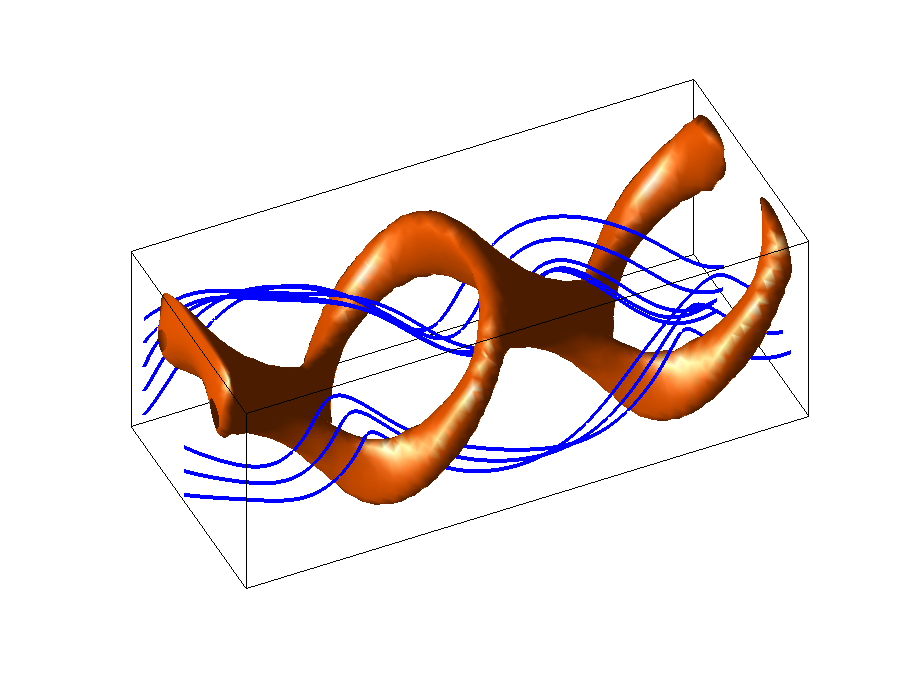
\includegraphics[width=0.5\textwidth]{example1structure2}}
    \caption{\label{example1structure} The left figure shows how $\alpha$ grows versus iteration on a line. It demonstrates that the material can be added in or taken out. The structure to maximize the downward velocity at the center of the channel after $46$ iterations is shown in the right figure. }
  \end{figure}

We use the simulation method we proposed to simulate this
system. The result is shown in Figure \ref{example1simulation}. The
system is clearly doing the right thing (maximizing the downward
velocity at the center of the channel).

  \begin{figure}
    \centerline{
     \includegraphics[width=1\textwidth,trim=0cm 0cm 0cm 7cm,clip]{example1simu}
     }
    \caption{\label{example1simulation} The cross-section simulation of the structured channel shown in Figure \ref{example1structure}.}
  \end{figure}

%%%%%%%%%%%%%%%%%%%%%%%%%%%%%%%
\subsection{A mixing channel }
%%%%%%%%%%%%%%%%%%%%%%%%%%%%%%%
In this example, we want to show how the use of a $g_1$ kind of
objective function can help us to design a mixing channel to realize
chaotic mixing. Stroock, et al.\ \cite{Stroock2002} proposed a
staggered herringbone mixer composed of two sequential
regions of ridges; the direction of asymmetry of the herringbones
switches with respect to the center-line of the channel from one region
to the next. The herringbone structure is fabricated with two steps of
photolithography and is located on the floor of the poly channel.
Experiments show that the length of the channel required for mixing
grows only logarithmically with $\text{Pe}$, instead of linearly as
in a smooth channel. The goal of the herringbone structure is to
produce transverse flows for which we can further optimize by the
$g_1$ objective function.

The mixing channel has dimension $(\ell_x,\ell_y,\ell_z) =
(0.06,0.01,0.02)\,$cm per period and is discretized into
$(n_x,n_y,n_z)=(144,24,48)$ grids. We set $c$ to maximize the downward
(negative $y$ direction) velocity inside the block
$[0,\ell_x]\times[0,\ell_y]\times[\frac{2}{6}\ell_z,\frac{5}{6}\ell_z ]$, which
can produce larger and smaller vortices. We consider two
scenarios: the material is restricted to be on the bottom of the
channel (the block $[0,\ell_x]\times[0,0.2\ell_y]\times[0,\ell_z]$), and the
material can be put anywhere inside the channel. The optimal
structures of both scenarios, as shown in Figure
\ref{example2structureNew}, contain several periods of (almost) the
same structure. The same pattern repeats four times in the first case
and three times in the second case. One can see that for the first
scenario, the optimal structure is also a herringbone type, but has a
higher frequency for the smaller vortex. For the second scenario, the
structure is formed by much more material and also tends to have a
higher frequency for the smaller vortex.


Just like in the previous example, one can simulate how the channel
mixes the colors by the Markov Chain model. However, in order to
produce chaotic mixing, the mixer has to be composed of two sequential
regions that are symmetric with respect to the plane
$z=\frac{1}{2}\ell_z$, and this breaks the periodic boundary condition
assumed in obtaining the Markov Chain. In order to perform a correct
simulation, one needs to solve the flow field for a full cycle of
channel.

Let us focus on the first scenario. Since the same structure repeats
four times in the solution, we take one of them and call it ``L''
(with dimension $(\ell_x,\ell_y,\ell_z)=(0.015,0.01,0.02)\,)$cm. The symmetric
structure of ``L'' is thus called ``R''. One can build an $n$-cycle
channel by connecting $n/2$ L structures and $n/2$ R structures
together. It thus has the period $0.015n\,\text{cm}$. For fixed
$\text{Pe}=1.2 \times 10^4$, we solve the flow field for different
$n$-cycles with $n=6$, $8$, $10$ and $12$, and find that when $n=8$,
the channel has the best mixing. Hence in Figure
\ref{example2trajectory}, the 8-cycle mixing channel is used to
perform the simulation with different $\text{Pe}$. We adjust
$\text{Pe}$ by changing the FFT/IFFT diffusivity between each
$8$-cycle ($0.12\,\text{cm}$). The trajectories have the same tendency
as the experiment results in the Figure 3(D) in \cite{Stroock2002}.
Define mixing length ($x_{90}$) as the channel length required for the
standard deviation to drop to $0.05$ (shown by a dashed line in Figure
\ref{example2trajectory}). The mixing length grows linearly with
$\log(\text{Pe})$, which also matches the experiments done in
\cite{Stroock2002}.


In Figure \ref{example2simu} we show some cross-sectional plots of two of
the simulations in Figure \ref{example2trajectory}, where the channel
is 8-cycle and $\text{Pe}$ are $1.2\times10^6$ and $1.2\times10^9$,
respectively. The first four plots of each case show the cross-section
at the end of the 1st to the 4th cycle, and the last plot for each
case shows the cross-section at the end of the 9th cycle. From this
comparison one can clearly see how the chaotic mixing protocol helps
color mixing even when diffusion is very small.


As for the 3-D structure, the best $n$-cycle we find is $n=2$
($\ell_x=0.04\, \text{cm}$) because this structure stirs the flow a lot.
To further compare our optimized structures and the design in
\cite{Stroock2002}, we also perform a simulation of Stroock's
staggered herringbone mixer. The mixing length versus
$\log({\text{Pe}})$ for the three simulations and the experiment data
given in \cite{Stroock2002} are plotted in Figure
\ref{example2mixinglength}. One can see that our simulation ($\times$)
has a longer mixing length comparing with the experiment
data ($\lozenge$) when $\text{Pe}$ is small, and they agree well when
$\text{Pe}\approx 10^6$ ($\log(\text{Pe})=14$). For even larger
$\text{Pe}$, the simulation is a reasonable linear extension of the
experiment data. As for the optimal mixing channel we suggest
($\square$ for the herringbone, and $\bigcirc$ for the 3-D structures), they
both significantly outperform Stroock's design.

In Figure \ref{example2crosscompare} (a) and (b), for
$\log(\text{Pe})=14$, the cross-section at the end of the $5$-th cycle
of our optimal herringbone solution and Stroock's design are plotted.
One can compare the simulation in Figure \ref{example2crosscompare}(b)
with Figure 3(C) in \cite{Stroock2002} to see how similar they are.
This justifies our Markov Chain model is valid when the diffusion is
small.


For the above two cases, the average flow velocity in the $x$
direction are both around $1.2\, \text{cm} \,\text{s}^{-1}$. We use
the same body force for the simulation of the optimal $3$-D structure,
and adjust the diffusivity to make $\log(\text{Pe})=14$. The optimal
$3$-D structure has a much shorter cycle length
($\ell_x=0.04\,\text{cm}$). Hence we plot the cross-section of it at the
end of $15$-th cycle in Figure \ref{example2crosscompare}(c). It shows
that when $x=0.6\, \text{cm}$, the colors have a much better mixing
than both herringbone type channels. However, since there is more
material stuffed inside the channel, for the same body force, the
average flow velocity in the 3-D structure channel is only $0.2\,
\text{cm} \,\text{s}^{-1}$--six times slower than the herringbone type
channels. Hence when we plot the cross-section of this mixing channel
at time $t=0.7s$ in Figure \ref{example2crosscompare}(d), it is not
significantly better than the other two channels at $t=0.5\,s$ and
$t=0.6\,s$. This says if one cares more about mixing time rather than mixing length, 
the $3$-D structure may not be the preferable choice. 

\todo{TC: Figure \ref{example2structureNew} needs to correct the unit.}

%%%%%%%%%%%%%%%%%%%%%%%%%%%%%%%%%%%%%%%%%%%%%%
% structure plot
  \begin{figure}
    \centerline{
     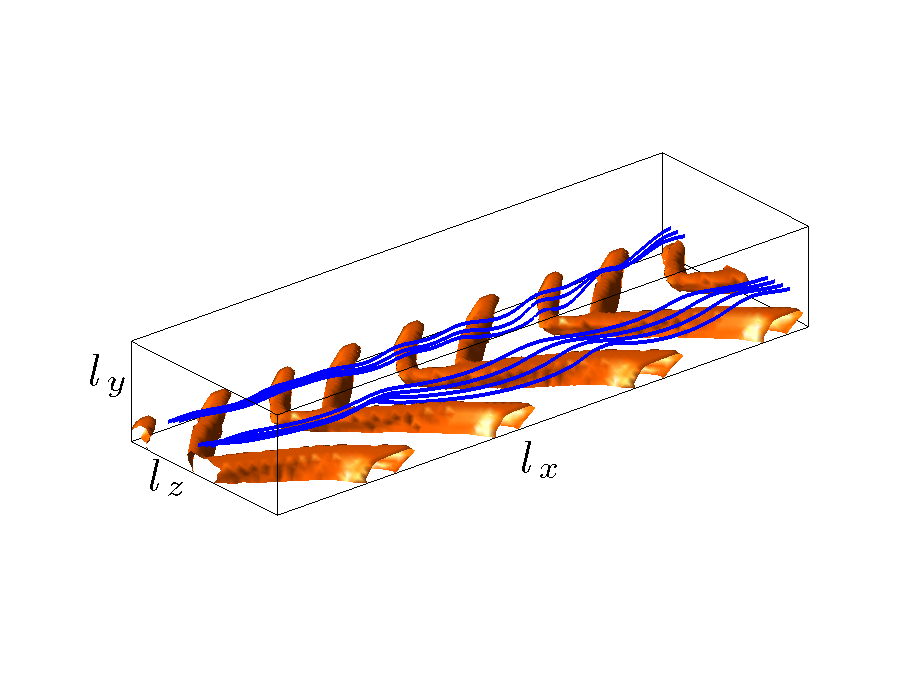
\includegraphics[width=0.5\textwidth]{example2structureherringbone}
     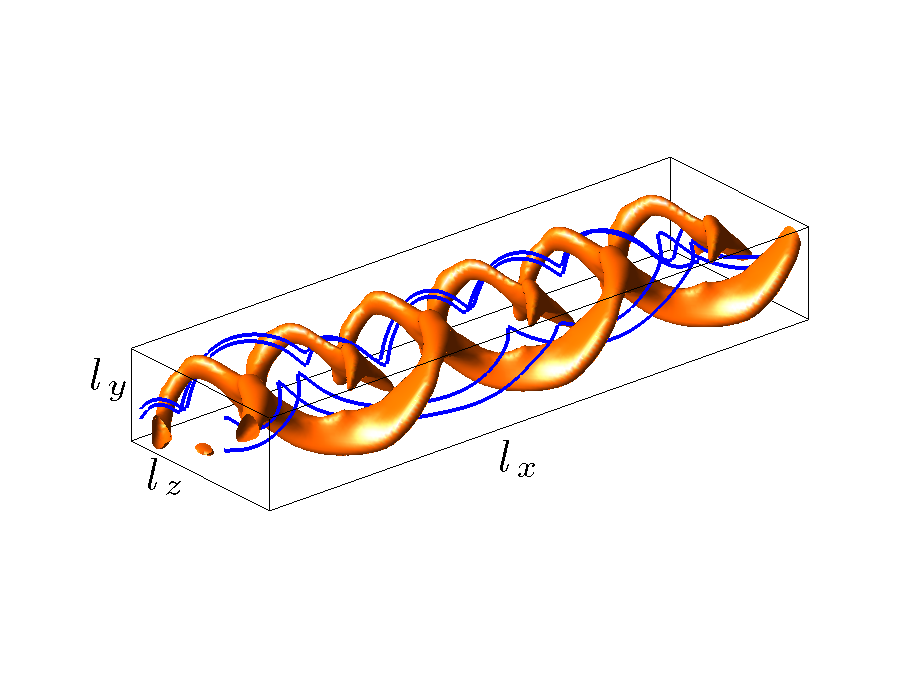
\includegraphics[width=0.5\textwidth]{example2structure3d}
     %\scalebox{0.6}[0.6]{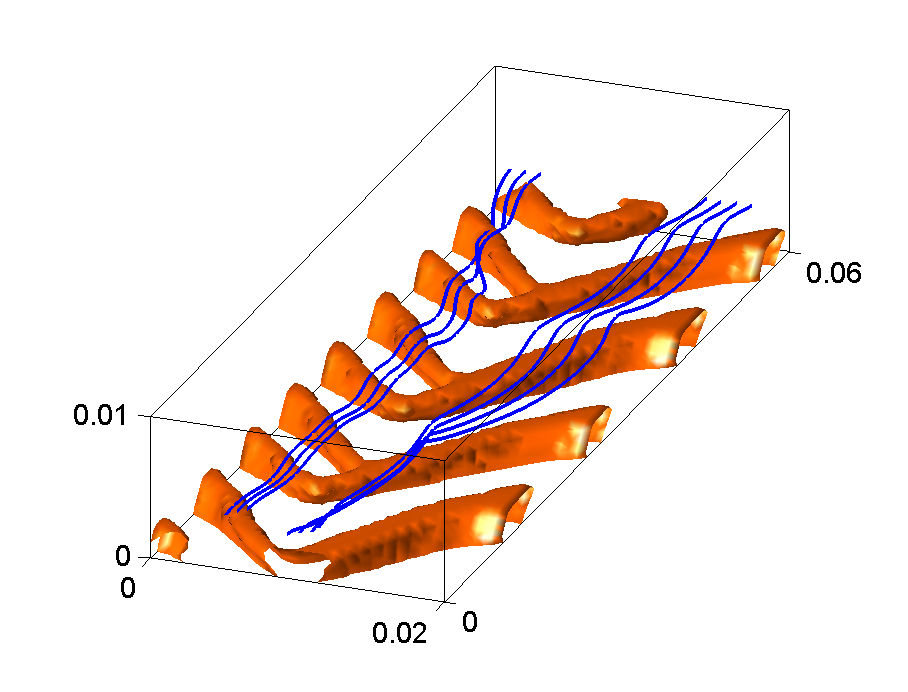
\includegraphics{myharringbonestructure}}
     %\scalebox{0.6}[0.6]{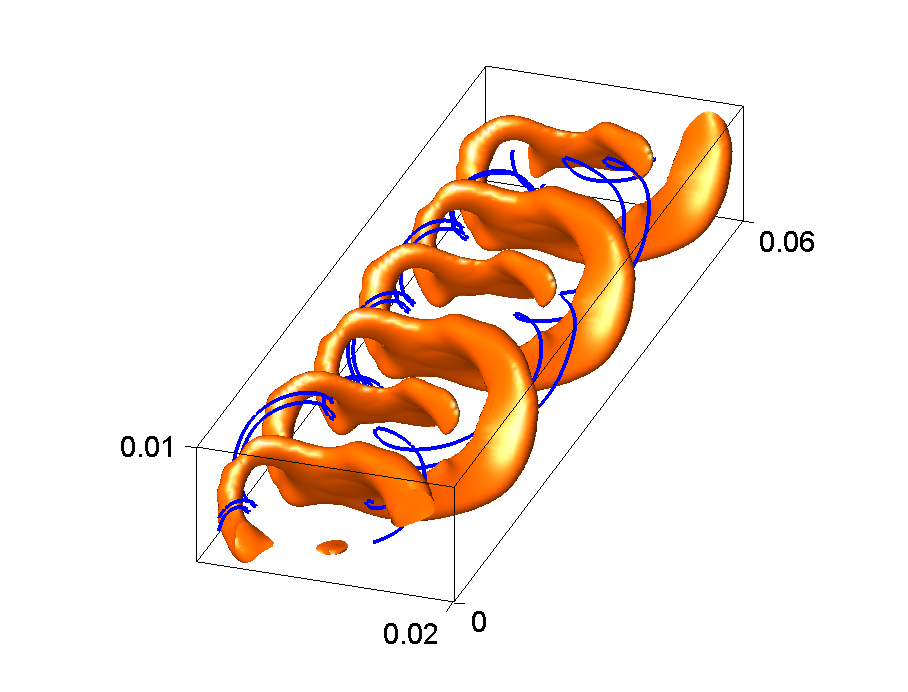
\includegraphics{my3dstructure}}
      }
    \caption{\label{example2structureNew} These two figures show the optimal channel structures to produce one big and one small vortex. For the left one we restrict the material to be on the bottom of the channel, and it forms a herringbone type structure. For the right one the material can be put anywhere inside the channel.}
  \end{figure}
%%%%%%%%%%%%%%%%%%%%%%%%%%%%%%%%%%%%%%%%%%%%%%%

%%%%%%%%%%%%%%%%%%%%%%%%%%%%%%%%%%%%%%%%%%%%%%%
%mixing trajectory
  \begin{figure}
    \centerline{
     %\scalebox{0.5}[0.5]{\includegraphics{example2veryCycles}}
     \includegraphics[width=0.58\textwidth]{example2veryPe2}}
    \caption{\label{example2trajectory} In this figure we vary $\text{Pe}$ by changing $D$ and use the $8$-cycle optimal herringbone structured channel for simulation. The mixing trajectories stay almost $0.5$ for a longer distance when $\text{Pe}$ is large.}
  \end{figure}
%%%%%%%%%%%%%%%%%%%%%%%%%%%%%%%%%%%%%%%%%%%%%%%

%%%%%%%%%%%%%%%%%%%%%%%%%%%%%%%%%%%%%%%%%%%%%%%
%cross-section simulation 1, for different Pe
  \begin{figure}
    \centerline{
     \includegraphics[width=1\textwidth]{example2simu2} 
    }
    \caption{\label{example2simu} For $\text{Pe} = 1.2\times10^6$ (left) and
$1.2\times10^9$ (right), we plot the cross-sections of the end of the
1st to the 4th cycle for both cases. The bottom two plots show the
cross-sections of the end of the 9th cycle for both cases. }
  \end{figure}
%%%%%%%%%%%%%%%%%%%%%%%%%%%%%%%%%%%%%%%%%%%%%%%

%%%%%%%%%%%%%%%%%%%%%%%%%%%%%%%%%%%%%%%%%%%%%%%%
% mixing length vs Pe, 4 cases
  \begin{figure}
    \centerline{
     \includegraphics[width=0.58\textwidth]{example2mixinglength2}
    }
    \caption{\label{example2mixinglength} The mixing length ($x_{90}$) is defined as the
    channel length required for the standard deviation to drop from $0.5$ to $0.05$
    (see the dashed line in Figure \ref{example2trajectory}). In this figure, we plot
    $x_{90}$ versus \text{Pe} for four different cases.
  $\lozenge$: the experiment data given in \cite{Stroock2002}; $\times$: our simulation
  using the design given in \cite{Stroock2002}; $\square$: our optimal herringbone type
  mixing channel, and $\circ$: our optimal 3-D structured channel. In all cases, $x_{90}$
  grows logarithmically with $\text{Pe}$. The simulation ($\times$) agrees well with the
  experiment ($\lozenge$) when $\text{Pe}$ is large, and the two optimal designs have shorter mixing lengths compared with Stroock's design.}
  \end{figure}
%%%%%%%%%%%%%%%%%%%%%%%%%%%%%%%%%%%%%%%%%%%%%%%%

%%%%%%%%%%%%%%%%%%%%%%%%%%%%%%%%%%%%%%%%%%%%%%%%
% cross-section comparison for 3 cases.
  \begin{figure}
    \centerline{
     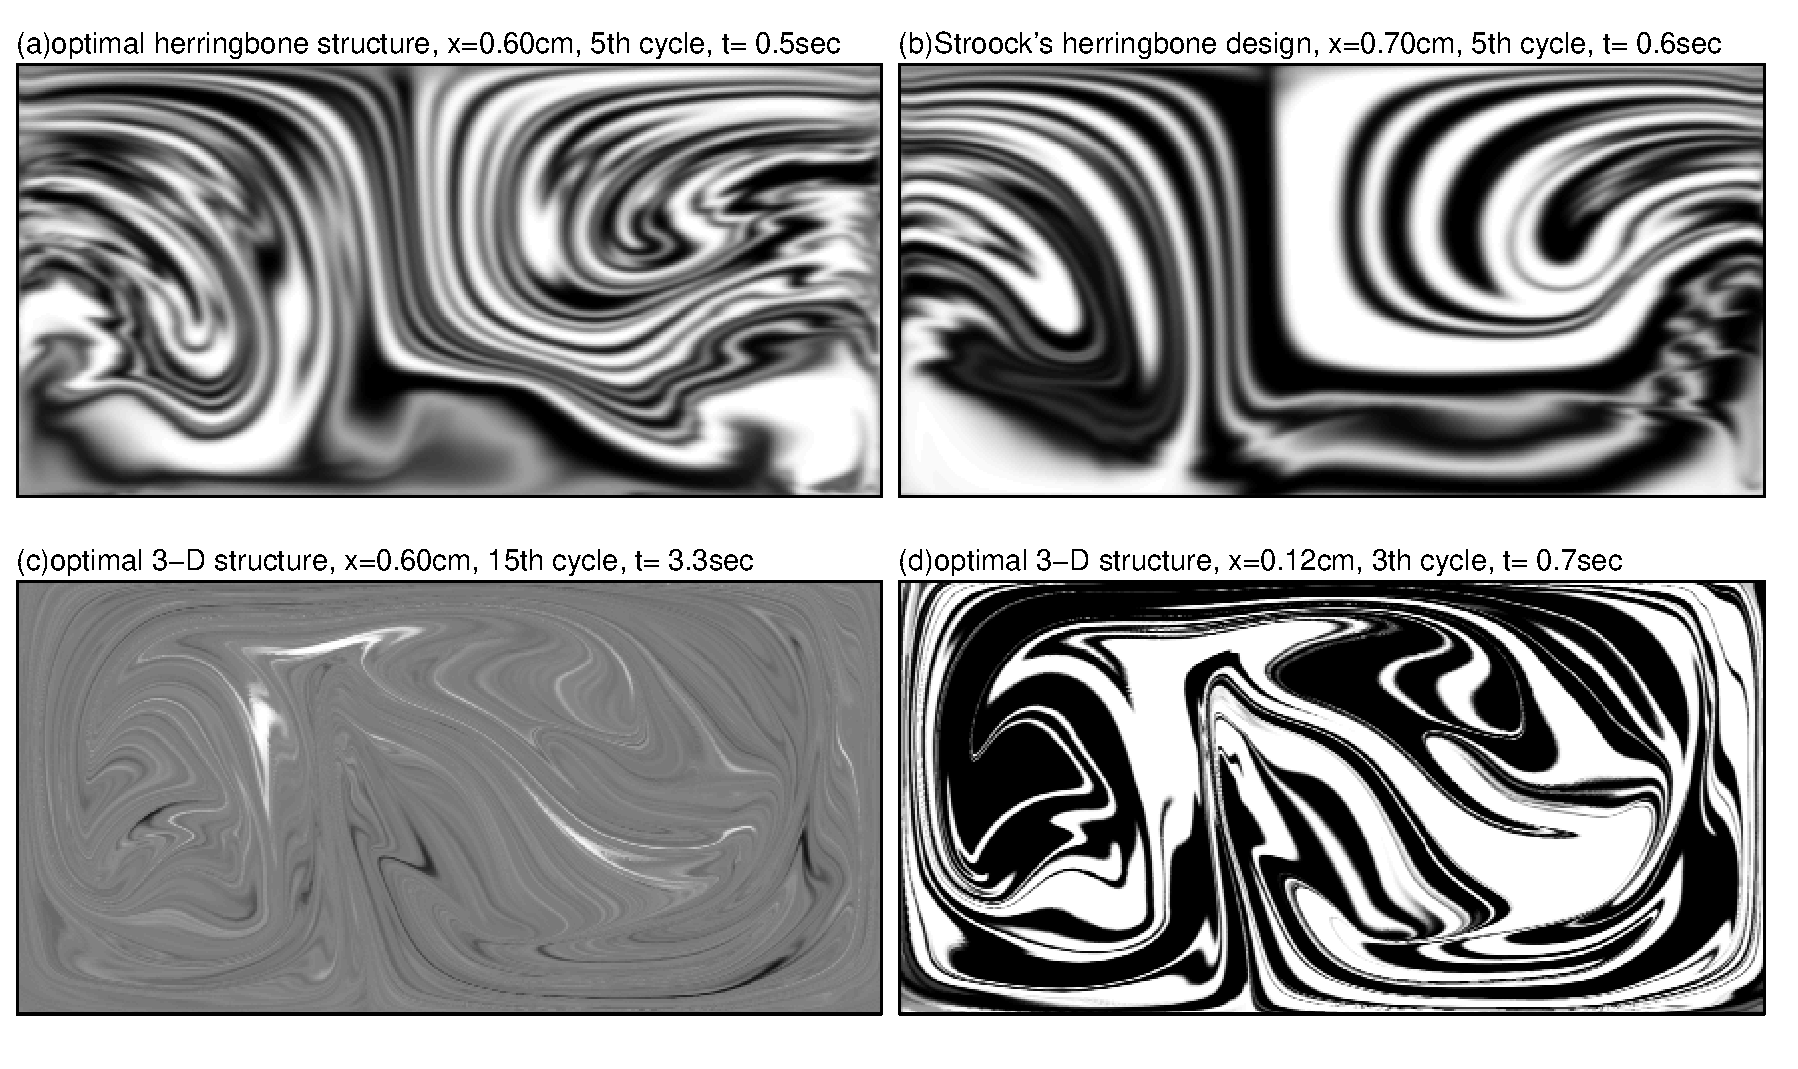
\includegraphics[width=1\textwidth]{example2crosscompare}
    }
    \caption{\label{example2crosscompare} Four cross-section plots: (a) the optimal herringbone structure at the end of its $5$th cycle; (b) the simulation of Stroock's herringbone design at the end of its $5$th cycle; (c) the optimal $3$-D structure at the end of its $15$th cycle; and (d) the optimal $3$-D structure at the end of its $3$th cycle. The color distribution in (b) is almost the same as the experimental result shown in Figure 3(C) in \cite{Stroock2002}. This demonstrates that our numerical methods are valid for simulating the true physical mixing process. Plots (c) and (d) show that although the $3$-D structure has a much smaller mixing length ($x_{90}$), it also drags the flow much more. For the same body force, the average velocity in the $x$-direction is only $1/6$ compared with the herringbone type structures. Hence for the same mixing time, the $3$-D structure is not better than the herringbone structures.}
  \end{figure}
%%%%%%%%%%%%%%%%%%%%%%%%%%%%%%%%%%%%%%%%%%%%%%%%

 % \begin{figure}
 %   \centerline{
 %    \scalebox{0.6}[0.6]{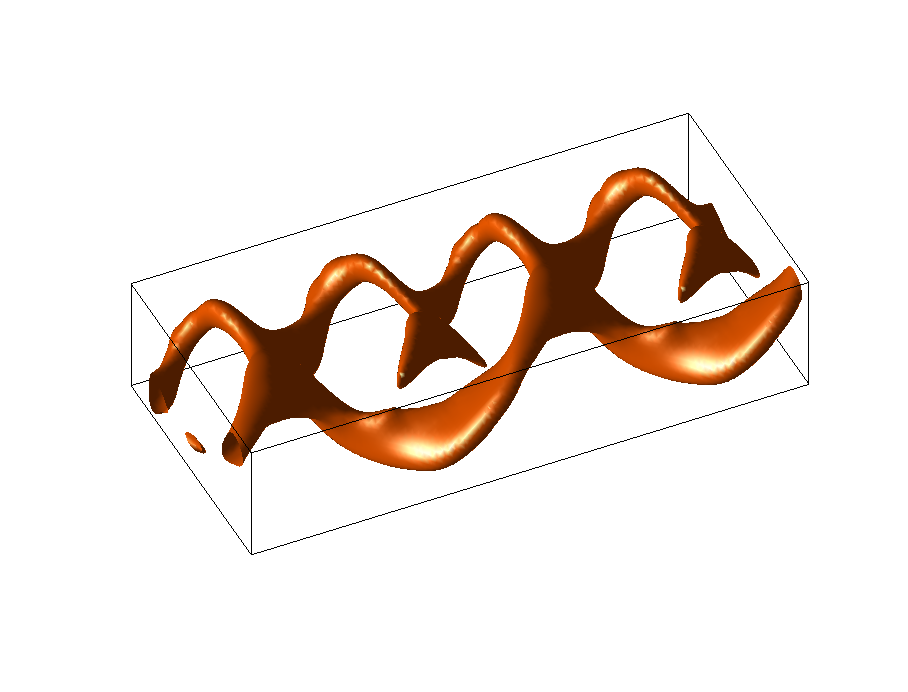
\includegraphics{example2structure}}
 %    \scalebox{0.6}[0.6]{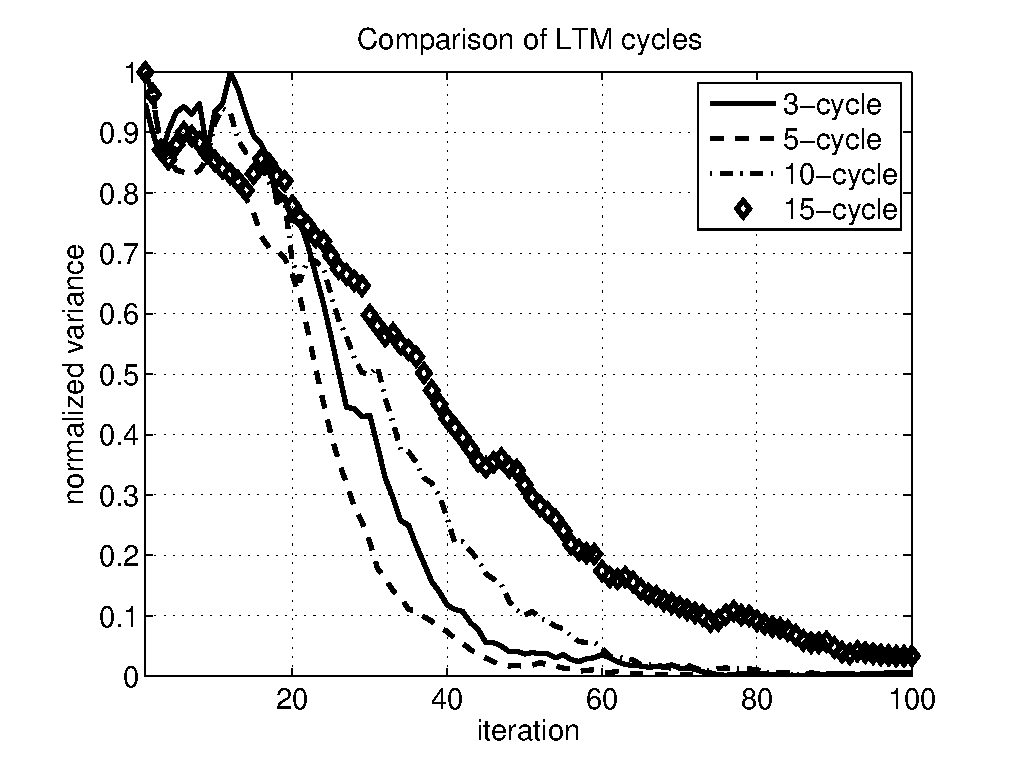
\includegraphics{ltmcompare}}}
 %   \caption{}
 % \end{figure}

 % \begin{figure}
 %   \centerline{
 %    \scalebox{0.6}[0.6]{\includegraphics{ltmsimulation}}
 %   }
 %   \caption{}
 % \end{figure}


%%%%%%%%%%%%%%%%%%%%%%%%%%%%%%%
\subsection{Designing a map}
%%%%%%%%%%%%%%%%%%%%%%%%%%%%%%%
As we have demonstrated in the previous example, the objective
function $g_1$ is really handy in the mixer design. However,
``maximizing the transverse velocity somewhere in the channel'' may
not always be a good strategy to achieve the flow we want. An ongoing
research area in chaotic mixing channel design is to realize a Linked Twist
Map. Similar to the staggered herringbone mixer, this mixing channel
is composed of two sequential regions of different channels. Each of
them is to twist the flow in a certain way and by adjusting the
arrangement of the two twist maps, one can achieve chaotic mixing. In
this type of design, we want the channel to rotate the flow for a
certain degree centered at a certain axis. The twist angle and the center
location are both important to create chaotic mixing. To realize such
a twist map, we can use the objective function $g_2$.

There are various kinds of twist maps, for example, $S(y,z;y_c,z_c,\theta): (y,z)\mapsto (y_e,z_e)$, and
\begin{align*}
   y_e &= y_c + r \cos(\alpha+\theta), \\
   z_e &= z_c + r \sin(\alpha+\theta), 
 \intertext{where}
   \alpha &= \text{atan2}(y-y_c,z-z_c), \\
   r      &= \sqrt{(y-y_c)^2 +(z-z_c)^2}.
\end{align*}
This defines a twist map centered at $(y_c,z_c)$ and with fixed
angle of rotation along the radius. This is of course not a realistic
map for a channel because it does not consider the non-slip boundary
conditions on the channel walls. However, we would like to see how far
a flow map can go. Again, the mixing channel has dimension
$(\ell_x,\ell_y,\ell_z) = (0.02,0.01,0.01)\,$cm per period, and is discretized
into $(n_x,n_y,n_z)=(64,32,32)$ grids. We use the objective function
$g_2$ for the above desired map and set $(y_c,z_c) =(0.5\ell_y, 0.5\ell_z)$.
The structure after $40$ iterations is shown in the left of Figure
\ref{example3figure1}. A set of streamlines starting from $41 \times
41$ regular mesh are calculated, and the end points, which form the
twisted grids, are plotted in the right of Figure
\ref{example3figure1}. The extra-thick line shows a block whose edges
are originally parallel to the channel walls and now rotated almost $45$
degrees. In Figure \ref{example3figure2} we show the simulation of
this channel. In the first $7$ iterations one can see how it rotates
the boundary between the colored liquids by roughly $45$ degrees. The
last plot in Figure \ref{example3figure2} shows the color field at the
$100$th iteration. Obviously, this channel does a bad job in mixing.

Unlike the objective function $g_1$, the optimal structure of this
problem is not solid. To actually fabricate this structure, porous
material is needed.

  \begin{figure}
    \centerline{
     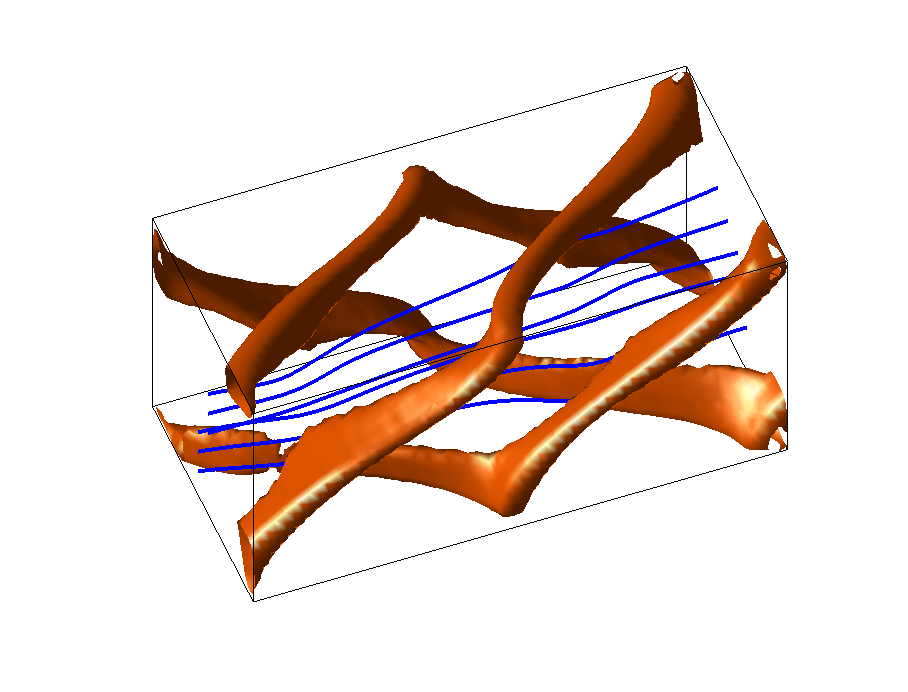
\includegraphics[width=0.5\textwidth]{example3structure}
     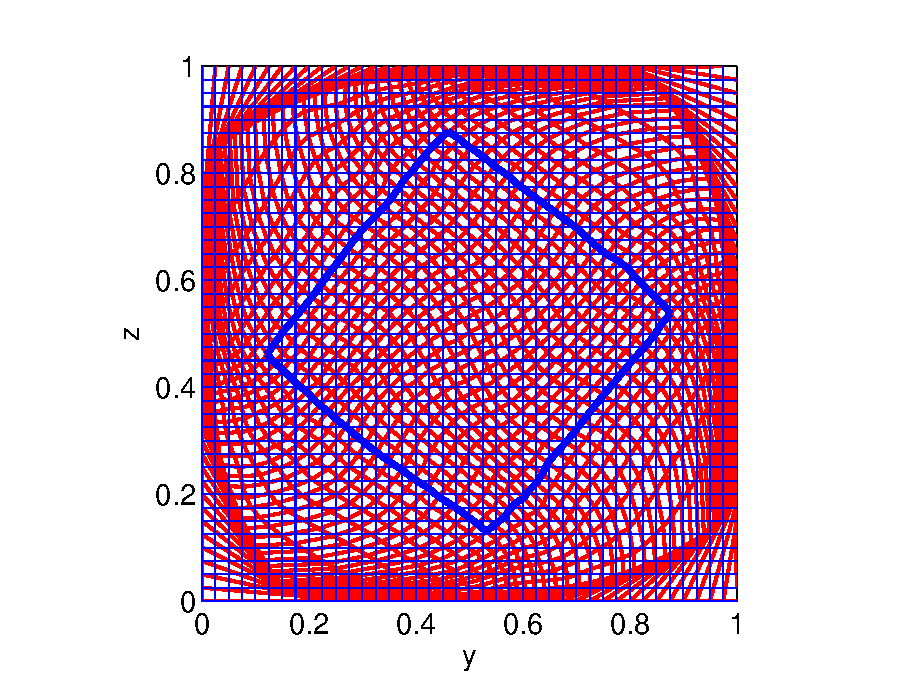
\includegraphics[width=0.5\textwidth]{example3grid}}
    \caption{\label{example3figure1} The left figure shows the optimal structure to twist the flow $45$ degrees. Note that the structure is not solid. The right figure shows the simulation of this twist channel for one period. A set of streamlines starting from $41$ by $41$ points on regular mesh grids are calculated, and the twisted grids on the other side of the channel are plotted. An extra-thick line shows a block whose edges are originally parallel to the channel boundary and now rotated roughly $45$ degrees.}
  \end{figure}


  \begin{figure}
    \centerline{
   \includegraphics[width=0.9\textwidth,trim=0cm 0cm 0cm 7cm,clip]{example3simu}}
    \caption{\label{example3figure2} The simulation of the optimal structure to rotate the flow field $45$ degrees. Clearly for the first $6$ periods, the flow field is rotated $45$ degrees per period. The last plot shows the cross-section at the $100$th iteration.}
  \end{figure}

%%%%%%%%%%%%%%%%%%%%%%%%%%%%%%%%%%%%%
%\subsection{Another linked twist map}
%%%%%%%%%%%%%%%%%%%%%%%%%%%%%%%%%%%%%
%In this example we use $g_2$ objective function to design $2$ maps: $S_1(y,z;y_{c_1},z_{c_1},\theta_1)$ and $S(y,z;y_{c_2},z_{c_2},\theta_2)$, where $\{y_{c_1},z_{c_2},\theta_1\}= \{0.3\ell_y,0.3_lz,\pi/4\}$ and $\{y_{c_1},z_{c_2},\theta_1\}= \{0.7\ell_y,0.7_lz,\pi/4\}$. We find the optimal structures, and then connect them to realize a linked twist map. The connected channel is shown in figure X. The velocity field is solved again for the new channel and now the period is doubled. The simulation of this mixing channel is shown in figure X. For comparison, we also simulate the system by using each of their twist maps.

%
% Conclusion
%
\section{Conclusion}
\label{sec:topoptconclusion}

We demonstrate how topology optimization can be applied to design the
flow field of a periodical microfluidic channel. The objective
function can be either a function of velocity components or a distance
between flow maps. A probabilistic model is also proposed to
approximate the solution of Advection-Diffusion equation on the
cross-sections of the mixing channel. We demonstrate the feasibility
of this model by reproducing the experiment results given in
\cite{Stroock2002}. Through topology optimization, the channel
structure is further improved and the mixing length is reduced by a
factor around $30\%$ and $60\%$ for the herringbone and $3$-D
structures, respectively.

Although we believe a further improvement can be made by designing
flow maps, it is shown by example $3$ that the local optimal structure
to realize a flow map is not likely to be a solid (black/white) one.
This suggests that if porous material is allowed in the fabrication of
microfluidic channels, one would have much more freedom in realizing
desired mixing protocols.

As one has seen, we use optimization techniques to assist the design or the realization of a mixing
protocol. The question may arise: is it possible to form an optimization problem such that the
objective function is a measure of how good the mixing protocol is? We have no good answer so far.
The difficulty we encounter is that there is no good measure about how well an operator is in terms
of mixing. One can use variance or mix-norm \cite{Mezic2005} to measure whether the color on the
cross-section of the channel is well mixed, but the link between this and a mixing protocol is
still missing. A potential solution to this question is the second largest eigenvalue
modulus (SLEV) \cite{Boyd2004} of the operator $A_n$. Clearly, for a fixed $n$, it determines how
fast the Markov Chain converges to its invariant distribution, so does the dual process---the
evolution of the color intensity to uniform. If one can minimize the SLEV of $A_n$ for one period of
the mixing channel, this gives a better mixing channel in the worst case scenario---if the initial color distribution is in an eigenvector direction. However, for the mixing trajectory shown in Figure \ref{example2trajectory}, the SLEV certainly determines the stationary slope of these trajectories, but not the transient part, and the mixing distance is almost completely decided by the transient phenomena. In fact, it has been shown that when the Markov transition matrix is non-normal or one uses different norms, the transient phenomena may be unrelated to the spectra (eigenvalues) of $A_n$, and have nontrivial relation to the pesudospectra \cite{Lloyd2005}. The famous example is called ``cutoff phenomenon'' in finite Markov Chain studies \cite{Diaconis1996, Diaconis2005, LSaloff-Costt2004}, and it has some interesting relation to chaotic mixing \cite{numcutoff, symdyn}.

Consider the mixing length shown in Figure \ref{example2trajectory}: when $\text{Pe}$ gets larger, the standard deviation stays high for a much longer
time before it begins to drop. So even though we know the mixing length grows logarithmically with $\text{Pe}$,
it does not mean we can cut the length of $x_{90}$ by half to get the mixing result by a factor
$0.5$---it is worse than that. These kinds of multi-stage mixing trajectories have been widely observed
and studied in chaotic map mixing.
See \cite{Thiffeault2003-13, Thiffeault2003-309, Thiffeault2004, Tsang2005, Haynes2005}
for examples. In \cite{numcutoff} the author studies Standard Map with small diffusion, and links
this multi-stage behavior of mixing process to the well-known cutoff phenomenon. Numerical evidence is provided to show that when the diffusion goes to zero, the mixing trajectoreis of the Standard Map with small diffusion perform a cutoff. The sharp change in the mixing trajectory certainly
describes the limit of chaotic mixing---it requires a minimal length for the mixing to occur.


%: denote the standard deviation as $\delta$. One can define the cutoff time of the mixing process to be the time required for $\delta$ to drop to $0.25$, and the window size to be
%the period from $\delta=0.45$ to $\delta=0.05$. The numerical evidence shows that for Standard map, when diffusion
%goes to zero, the windows size divided by the cutoff time also goes to zero. 



%%%%%%%%%%%%%%%%%%%%%%%%%%%%%%%%%%%%%%%%%%%%%%%%%%%%%%%%%%
%%%%%%%%%%%%%%%%%%%%%%%%%%%%%%%%%%%%%%%%%%%%%%%%%%%%%%%%%%
\chapter[Numerical Evidence of Cutoffs]{Numerical Evidence of Cutoffs in Chaotic Mixing}
%


In this chapter, we focus on the mixing process of Standard Map in the near-zero diffusion limit. We build a numerical strategy to simulate the map with very high resolution (up to $8 \times 10^4$ by $8 \times 10^4$ grids) and hence very low numerical diffusion. This numerical strategy is realized by a Markov Chain simulation. To characterize the behavior of the variance trajectory in the near-zero diffusion limit, the notion of cutoff in the study of finite Markov Chains is brought. We numerically show that the sequence of models presents a cutoff, which qualitatively characterizes the mixing process when the diffusion goes to zero. The attempt in this chapter is to build a bridge between finite Markov Chain studies and $2$-D chaotic maps with small diffusion. Analytical results of $1$-D chaotic maps with cutoff phenomenon is discussed in next chapter.

This chapter is organized as follows. In section \ref{sec:numcutoffbackground} we briefly review the background of the operators we use and the cutoff phenomenon. Section \ref{sec:modelreduction} provides a model reduction view of building the Markov Chain model of chaotic maps, and the actual numerical strategies we use in simulations. Numerical evidence of Standard Map cutoff is given in section \ref{sec:numresults} and a conclusion in section \ref{sec:numcutoffconclusion}.  



%
% Body
%

%%%%%%%%%%%%%%%%%%%%%%%%%%%%%%%%%%%%%%%%%%%%%%%%%%%%%%%%%%
%%%%%%%%%%%%%%%%%%%%%%%%%%%%%%%%%%%%%%%%%%%%%%%%%%%%%%%%%%
\section{Background}
\label{sec:numcutoffbackground}
%%%%%%%%%%%%%%%%%%%%%%%%%%%%%%%%%%%%%%%%%%%%%%%%%%%%%%%%%%
%%%%%%%%%%%%%%%%%%%%%%%%%%%%%%%%%%%%%%%%%%%%%%%%%%%%%%%%%%

%%%%%%%%%%%%%%%%%%%%%%%%%%%%%%%%%%%%%%%%%%%%%%%%%%%%%%%%%%
\subsection{The measure space and operators}
%%%%%%%%%%%%%%%%%%%%%%%%%%%%%%%%%%%%%%%%%%%%%%%%%%%%%%%%%%

We work on the probability space $(X,\mathcal{A},\mu)$. We take $S: X
\to X$ to be a transformation (or map) that is non-singular and
measurable. We choose $\mu$ to be the Borel measure. In the measure
space $(X,\mathcal{A},\mu)$ we define the following operators.
%\begin{definition} {\bfseries (Markov operator)}
%Any linear operator $M:L^1 \rightarrow L^1$ satisfying
%(a) $Mf \ge 0$ for $f\ge 0, f \in L^1$; and
%(b) $||Mf|| = ||f||$ for $f\ge 0, f \in L^1$
%is called a Markov operator.
%\end{definition}

\begin{definition}[Perron-Frobenius operator]
The Perron-Frobenius operator $P:L^1(X) \to L^1(X)$ associated with
$S$ satisfies
\begin{equation}
  \int_A (P \omega)(x)\mu(dx) = \int_{S^{-1}(A)} \omega(x)\mu(dx)
\end{equation}
for every $\omega \in L^1(X)$ and $A \in \mathcal{A}$.
\end{definition}
The Perron-Frobenius operator is linear. Because of our choice of
measure space, the Perron-Frobenius operator can be interpreted as a
map that evolves probability density functions. Also, suppose that
$\bar{\omega}$ is an invariant measure of $S$, so that
\begin{equation}
   \bar{\omega}(S^{-1}(A)) = \bar{\omega}(A)  \text{ for all } A \in \mathcal{A}.
\end{equation}
Then we have (omitting $x$)
\begin{eqnarray}
  P \bar{\omega} = \bar{\omega}.
\end{eqnarray}
%Suppose $S$ is invertible and since it is measure preserving, we have
% \begin{eqnarray}
% P_Sf(x) = f(S^{-1}(x))
% \end{eqnarray}

\todo{MW: I changed ``the invariant measure'' to ``an invariant
  measure''. It isn't generally unique?}

\todo{MW: For consistency we should always write $P(\omega)$ or $P
  \omega$. I tend to value the latter to suggest its linearity.}

\begin{definition}[Koopman operator]
Let $f \in L^\infty(X)$. The operator $U:L^{\infty}(X) \to
L^{\infty}(X)$ defined by
 \begin{eqnarray}
 Uf(x) = f(S(x))
 \end{eqnarray}
is called the Koopman operator associated with $S$.
\end{definition}
The Koopman operator is adjoint to Perron-Frobenius operator, which we
write as $U = P^*$.

\todo{MW: I added the domain to the function spaces above, so we have
  $L^\infty(X)$ rather than just $L^\infty$. Should we also add the
  range to make it completely clear? That is,
  $L^\infty(X,\mathbb{R})$?}

%%%%%%%%%%%%%%%%%%%%%%%%%%%%%%%%%%%%%%%%%%%%%%%%%%%%%%%%%%
\subsection{Notion of a cutoff}
%%%%%%%%%%%%%%%%%%%%%%%%%%%%%%%%%%%%%%%%%%%%%%%%%%%%%%%%%%

In some Markov Chains, certain probability distributions converge to
an equilibrium via a sharp transition, which becomes sharper for
larger chains. This phenomenon is referred to as \emph{cutoff} in the
finite Markov chain literature \cite{Diaconis2005, Chen2006}. Here we
extend the usual definition slightly to accommodate converge to
non-zero distance values.

\todo{MW: Why don't we compute the variance of the $f^k_n$ after
  subtracting the invariant distribution, or something, so that we
  really converge to zero?
  
  TC: We discussed this before. When the diffusion is not zero, the 
  stationary distribution is always uniform. However, Standard Map 
  has non-chaotic regions, so as the diffusion decreases, each of the 
  trajectories in Figure 2 goes to zero with decreasing exponential 
  decay rate (the second largest eigenvalue). And even in the 
  normalized plot, the decay rate is still decreasing, so for fixed 
  $k/t_n$ (say, $k/t_n=3$), we can expect $\text{var}(f_n^k)$ to 
  converge to a constant, but it is not stationary. It is the 
  eigenvector connrsponding to the second largest eigenvalue. 
  }
  

\todo{MW: I think we should name this $d$ so that we can refer to it
  below in the definition of cutoff. Does it have a standard name? If
  not, maybe we should call it a distance function?}

To any finite set $\Omega$ and any pair of probability measures
$\omega$, $\bar{\omega}$ on $\Omega$ we associate a real number
$d(\omega,\bar{\omega})$ such that
\begin{subequations}
\label{eqn:defn_d}
\begin{align}
d(\omega,\bar{\omega}) &\in [0,1] \\
d(\omega,\bar{\omega}) &= 0 \text{ if and only if } \bar{\omega}=\omega \\
\max_{\Omega,\omega,\bar{\omega}} d(\omega,\bar{\omega}) &= M_d.
\end{align}
\end{subequations}
Note that $d$ need not satisfy the triangle inequality and so is not a
metric.

\todo{MW: Should the max above really be over all $\Omega$ as well? It
  seems to be we only have one $\Omega$.}

\todo{MW: Should the max above be a sup? Why do we know the max is
  achieved?}

\todo{MW: Check that the not-a-metric comment above is correct.}

Consider a sequence of finite probability spaces $(\Omega_n)$ for $n =
1,2,\ldots$. We think of $n$ as the size of the space. Each space is
equipped with a probability measure $\bar{\omega}_n$ which we think of
as the unique invariant measure of a Markov chain on $\Omega_n$. For
each $n$ we now take a sequence of probability measures $\omega_n^k$
for $k = 0,1,2,\ldots$ such that
\begin{equation}
\lim_{k \rightarrow \infty} d(\omega_n,\bar{\omega}_n)=0.
\end{equation}
The $\omega_n^k$ should be thought of as an initial condition
$\omega_n^0$ and then iterates of the distribution under the
evolution of a Markov chain.

\todo{MW: The above paragraphs are a bit of a mess, but somehow I
  wanted to explain what the objects are. Do we want the $\omega$ to
  be pdfs, or do we rather want them to be functions on $\Omega$?}

\todo{MW: Use ldots ($\ldots$) rather than $...$ to get better
  spacing.}

The definition of a cutoff follows.
\begin{definition}[Cutoff]
\label{cutoffdefinitionn}
Take a family $(\Omega_n,\bar{\omega}_n,
(\omega^k_n)_{k=0}^{\infty})_{n=1}^{\infty}$ of finite probability
spaces $\Omega_n$ and probability measures $\bar{\omega}_n$ and
$\omega_n^k$. This family presents a $d$-cutoff if there exists a
sequence $(t_n)_{n=1}^{\infty}$ of positive reals such that, for any
$\epsilon \in (0,1)$,
\begin{subequations}
  \label{eqn:defn_cutoff}
  \begin{align}
    \label{eqn:defn_cutoff_1}
    \lim_{n \rightarrow \infty}d(\omega^{k_n}_n,\bar{\omega}_n) &= m \text{ if }
    k_n > (1+\epsilon)t_n \\
    \lim_{n \rightarrow \infty}d(\omega^{k_n}_n,\bar{\omega}_n) &= M \text{ if }
    k_n < (1-\epsilon)t_n
  \end{align}
\end{subequations}
\end{definition}

\todo{MW: Should we define the $t_n$ to be \emph{cutoff times}?}

\todo{MW: In the cutoff definition we don't say what the $k_n$
  are. This needs to be clarified.}

\todo{MW: Remind me why we need the $\epsilon$ in the cutoff
  definition? Why can't we just say $k_n > t_n$ and $k_n < t_n$?}

This definition is taken from \cite{Diaconis2005} with the change that
$m$ and $M$ are $0$ and $M_d$ in the original. The reason for this
modification will be clear when we present the results of Standard Map
simulation.

The definition of cutoff implies that the change of
$d(\omega_n^k,\bar{\omega}_n)$ from $M$ to $m$ happens ever more
rapidly as $n$ increases, but only in relation to the cutoff times
$t_n$. We can think of this as rescaling the each trajectory
$(\omega_n^k)_{k=0}^{\infty}$ in time by $t_n$ and seeing cutoff as
the limit of these rescaled trajectories to a step function.

%%%%%%%%%%%%%%%%%%%%%%%%%%%%%%%%%%%%%%%%%%%%%%%%%%%%%%%%%%
%%%%%%%%%%%%%%%%%%%%%%%%%%%%%%%%%%%%%%%%%%%%%%%%%%%%%%%%%%
\section{A model reduction view and the numerical strategy}
\label{sec:modelreduction}
%%%%%%%%%%%%%%%%%%%%%%%%%%%%%%%%%%%%%%%%%%%%%%%%%%%%%%%%%%
%%%%%%%%%%%%%%%%%%%%%%%%%%%%%%%%%%%%%%%%%%%%%%%%%%%%%%%%%%

%%%%%%%%%%%%%%%%%%%%%%%%%%%%%%%%%%%%%%%
\subsection{A model reduction view}
%%%%%%%%%%%%%%%%%%%%%%%%%%%%%%%%%%%%%%%

In this section we explain the numerical strategy to perform the simulation in detail. It is based on a model reduction view of Perron-Frobenius and Koopman operators, and the Advection-Diffusion process is done by performing a Markov Chain/linear system simulation in a finite-dimensional space. Although we make this numerical strategy extremely simple in order to go up to very fine resolution, it is still worth to explain how we make the simplification step by step.     


Firstly, in the measure space $(X,\mathcal{A},\mu)$, given an invertible map $S$, let $P_S$ and $U_S$ be the Perron-Frobenius and the Koopman
operators of a map $S$. We have the following relations:
\vspace{0.15cm}
\begin{center}
\begin{tabular}{l|ll}
\label{PUtable}
& forward in time
& backward in time
\\
\hline
probability density
& $P_S$
& $P_{S^{-1}}$
\\
scalar function
& $ U_{S^{-1}} = P_{S^{-1}}^* $
& $ U_S  = P_S^*  $
\end{tabular}
\end{center}
\vspace{0.15cm}

\todo{MW: What are $A$ and $B$ here? The language below about
  ``infinite dimensional matrices'' is not mathematically meaningful
  and should be cut. It's fine to talk about $P_S$ and $U_S$ being
  dual, so long as they really are (check this).}
  
Note the above interpretation of the operators comes from the choice of $\mu$ to be the Borel measure. One can have different interpretation if the choice is different. Moreover, since $U_S$, $U_{S^{-1}}$, $P_S$, and $P_{S^{-1}}$ are all real linear operators, one can think them as matrices, and so $U_S$ is simply the transpose of $P_S$, so do $U_{S^{-1}}$ and $P_{S^{-1}}$. We can also find the relation between $P_S$ and $U_{S^{-1}}$:  
\todo{MW: Under what conditions does (\ref{ABrelation}) actually
  hold?}
\begin{eqnarray}
  \label{ABrelation}
        U_{S^{-1}}  = [\bar{\omega}^{-1}] \circ P_S \circ [\bar{\omega}],
\end{eqnarray}
where $[\bar{\omega}]f(x) =f(x) \bar{\omega}(x)$ and $ [\bar{\omega}^{-1}]f(x) =f(x)/ \bar{\omega}(x)$ for any function $f: X \to \mathbb{R}$. This result can be derived directly from the definition of the two operators. Therefore once we have obtained any one of the four operators, it is in general easy to find the other three.

The goal of this paper is to study how a scalar function is advected by a chaotic map in the near-zero diffusion limit. From the above table, the operator one needs in this situation is $U_{S^{-1}}$. For a given scalar function $f^0: X \to \mathbb{R}$, 
\begin{eqnarray}
\label{actualiteration}
 f^{k+1} = U_{S^{-1}} f^{k}, \text{ for all }k.
\end{eqnarray}
The way we actuall perform the iteration is we approximate $U_{S^{-1}}$ by a finite-dimensional Markov transition matrix $B_n \in \mathbb{R}^{n \times n}$, and use it to iterate  $f_n^0 \mathbb{R}^n $, an approximation of the given initial function. Thus,
\begin{eqnarray}
\label{approxiteration}
 f_n^{k+1} = B_n f_n^{k}, \text{ for all }k.
\end{eqnarray}
The difference between the approximate process (\ref{approxiteration}) and the actual one (\ref{actualiteration}) is treated as the numerical diffusion, and this numerical diffusion can be reduced by increasing $n$. Thus we can have a sequence of irreducible Markov transition matrices $B_n$ (and similarly $A_n$) which converge to $U_{S^{-1}}$ (and $U_S$) when $n$ goes to infinity. Each of the $B_n \in\mathbb{R}^{n \times n}$ represents a finite-dimensional approximation of $U_{S^{-1}}$. Because we treat the error between (\ref{approxiteration}) and (\ref{actualiteration}) as the added numerical diffusion, when $n$ goes to infinity, the numerical diffusion decreases to zero. The way to find $B_n$ for a given $U_{S^{-1}}$ is through the procedure of model reduction.

Begin with $B_n$. It evolves $f_n \in
\mathbb{R}^n$. We first define a map (an observer) $g_n: f(x) \mapsto
f_n $ such that
\begin{eqnarray} 
  (f_n)_i = (g_n(f(x)))_i = \int_{a_i} f(x) \mu(dx) \mbox{, for }i = 1
  \mbox{ to } n.
\end{eqnarray}
The sample space $X$ is discretized into $n$ grids $a_1,a_2,\ldots,a_n$ and each grids represents one state in the new sample space. There are various methods to find $B_n$ such that $\lim_{n\rightarrow \infty}B_n = U_{S^{-1}}$. One example is the lattice method \cite{Pierrehumbert2000}. It approximates $U_{S^{-1}}$ by a permutation
matrix, and then adds a smoothing step to make the matrix irreducible. In fact an optimal $B_n$ can be found by the techniques
of optimal model reduction \cite{Beck2007, Froyland2001, Froyland1999}: for any $f$ and $f_n = g_n(f)$, the optimal reduced
model of $U_{S^{-1}}$ is the $B_n$ such that
\begin{eqnarray}
\label{objfunction1}
  B_n f_n = \operatorname*{argmin}_{{f'_n}} || {f'_n} -g_n(U_{S^{-1}} f) ||_{\text{diag}(\sqrt{\bar{\omega}})},
\end{eqnarray}
i.e. it minimize the iteraiton error in the weighed norm space. Suppose the grids are numbered by $a_1,a_2,\ldots, a_n$. The optimal $A_n\in \mathbb{R}^{n \times n}$ satisfying~(\ref{objfunction1}) can be calculated explicitly as
  \begin{eqnarray}
    \label{Bnij}
    (B_n)_{ij} =  \frac{\bar{\omega}(S(a_j)\cap a_i)}{\bar{\omega}(a_j)}.
  \end{eqnarray}
To evaluate ($\ref{Bnij}$) requires the calculation of $S(a_j)$,
finding the area intersection, and integrating over a non-uniform
measure $\bar{\omega}$. For most of the maps, these steps can only be
done numerically.  Similarly, the optimal $A_n$, which is the best approximation of $U_S$, has the explicit form
  \begin{eqnarray}
    \label{Anija}
    (A_n)_{ij} =  \frac{\bar{\omega}(S^{-1}(a_j)\cap a_i)}{\bar{\omega}(a_j)}.
   \end{eqnarray}
One can check that the pair $\{A_n$, $B_n\}$ satisfies
 \begin{eqnarray}
  \label{AnBnrelation}
         B_n = \text{diag}({\bar{\omega}_n}^{-1}) A_n^T \text{diag}(\bar{\omega}_n),
  \end{eqnarray}
which is a discrete version of (\ref{ABrelation}). Apparently, how good
the approximation is for a certain $n$ depends on the choice of mesh
grids. In this article, we simply use regular grids: for $X =
[0,1]\times[0,1]$, each grid has size $h=1/\sqrt{n}$ in each
dimension and area $1/n$, $A_n \in \mathbb{R}^{n \times n}$.



%The proposed numerical strategy can be easily applied to 1-D maps, where $\bar{\omega}(S^{-1}(a_j)\cap a_i)$ is calculated by linear integration with measure $\bar{\omega}$ over the overlapping region of grids $S^{-1}(a_j)$ and $a_i$. For 2-D maps, numerical integration with measure $\bar{\omega}$ needs to be applied. This is in general very expensive and cannot be done for large number of grids. To give the feeling of how the number of girds relates to the approximation results, we use the mixing channel example again.

\todo{MW: The following example seems again to be irrelevant for the
  main point of the paper. I think reviewers will be confused by
  it. We should just directly define the method that we will use to
  generate the numerical results and cut the example below, I
  think. Just to make sure I understand things here, the numerical
  method described below and used for~\ref{mixingcrosssectionreduced}
  is not the method used to generate the final numerical results,
  right?}

The proposed numerical strategy can be easily applied to 1-D maps, where $\bar{\omega}(S^{-1}(a_j)\cap a_i)$ is calculated by linear integration with measure $\bar{\omega}$ over the overlapping region of grids $S^{-1}(a_j)$ and $a_i$. In 2-D, it is already hard to decide whether $S(a_j)\cap a_i$ is non-empty, let alone to calculating the areas. Therefore further simplification needs to be done for high resolution. In fact, when the grid gets smaller, the variation of $\bar{\omega}$ over one grid also becomes smaller, and one can safely approximate $B_n$ by
 \begin{eqnarray}
    \label{Anijapprox}
    (B_n)_{ij} \approx  \frac{{\mu}(S(a_j)\cap a_i)}{\mu(a_j)}.
   \end{eqnarray}
To go up to extremely high resolution, we make the approximation
procedure even simpler: suppose $X = T^2$ and $S: T^2 \rightarrow
T^2$, and let the grid size be $h$ on both dimensions. We number the grids
by $a_1,a_2,\ldots, a_{n^2}$. Let $\mathbf{x}_i =(x_{1i},x_{2i})$ be the
center of grid $a_i$; then
 \begin{eqnarray}
 \label{finegridmethod}
 (B_n)_{ij} \approx \begin{cases}
   \frac{1}{4} &\mbox{if } S(x_{1j}\pm \frac{h}{2},x_{2j}\pm \frac{h}{2}) \in a_i, \\
   0           &\mbox{otherwise}. \\
 \end{cases}
 \end{eqnarray}
To evaluate (\ref{finegridmethod}) we need only map points on the grid corners. The approximation of $B_n$ has only $4$ non-zeros in each row. Compared with (\ref{Bnij}), this approximation is far from optimal, but when $n$ goes to infinity, clearly it still converges to $U_{S^{-1}}$. During the simulation, the matrix $B_n$ is never explicitly
formed. We need only store a size $n$ state vector during the iteration. This approximation ensures that the operation count of evolving the system is always a constant times $n$. Equation~(\ref{finegridmethod}) will serve as our main tool in section~\ref{sec:numresults}. 

We want to stress again that although the numerical strategy we use is just equation~(\ref{finegridmethod}), the above simplification procedure is still necessary for understanding the insight of it. We apply a similar numerical strategy in~\cite{topopt} for the mixing process of a microfluidic mixing channel. The flow map generated by the microfluidic mixing channel does not have a uniform invariant distribution. In fact, the physical intrepretation of the invariant distribution is the normal velocity profile on the cross-section of the channel. Hence the choice of the operators to assure the correct physical conservation is thus crucial for the accuracy of the result. Refer \cite{topopt} for more detail.   

\todo{MW: When referencing things we should put a non-breaking space
  just before the ref, so that it doesn't get put on a separate
  line. For example, use section~\ref{sec:numresults} rather than
  section \ref{sec:numresults}. In the above paragraph the final
  section number was appearing by itself on a line until I added the
  non-breaking space.}

\todo{MW: We should have a figure like~\ref{mixingcrosssectionreduced}
  but for the standard map and using the numerical method that we
  actually use for the numerical results section.}


%%%%%%%%%%%%%%%%%%%%%%%%%%%%%%%%%%%%%%%
\subsection{Additional smoothing steps}
%%%%%%%%%%%%%%%%%%%%%%%%%%%%%%%%%%%%%%%
Using the numerical strategy in the previous section, we can evolve a function or a probability
distribution by the map with some small numerical diffusion. The effect of numerical diffusion is
similar to physical diffusion in large scale, but their behaviors can be quite different in 
small scale, and these small-scale phenomenon might be important for a chaotic map to form its
stationary eigenfunction. Therefore to simulate the physical diffusion correctly, we need to
simulate the map with far higher resolution with some additional diffusion added. The additional
diffusion can be added either in spatial or in frequency domain. In spatial domain, we adopt
the method of adding a smoothing step used in \cite{Tsang2005}:
 \begin{eqnarray}
 \label{smoothingstep}
   f^{k+1}_{(p,q)} = \sum_{|r|,|s|\le 2}C_{|r|}C_{|s|}f^{k}_{(p,q)}
 \end{eqnarray}
with $C_0=1/8, C_1=1/4$, and $C_2=3/16$ and $(p,q)$ the two dimensional index of the grid. This creates a large-scale diffusion $D \approx h^2$, which is several times larger than the numerical diffusion we originally have \cite{Tsang2005}. We use a smoothing operator $M_n$ and $f^{k+1} = M_n(f^{k})$ to denote the above smoothing step. Alternatively, in frequency domain a two-dimensional FFT/IFFT with multiplication by a constant in between according to the wave numbers can be applied to simulate physical diffusion, too. This procedure is denoted by an operator $F_n$ and $f^{k+1} = F_n(f^{k})$. Note that the FFT/IFFT scheme is much more expensive when $n$ is large, because massive data transfer is required between the first dimension FFT/IFFT and the second dimension FFT/IFFT.


%%%%%%%%%%%%%%%%%%%%%%%%%%%%%%%%%%%%%%%%%%%%%%%%%%%%%%%%%%
%%%%%%%%%%%%%%%%%%%%%%%%%%%%%%%%%%%%%%%%%%%%%%%%%%%%%%%%%%
\section{Numerical results}
\label{sec:numresults}
%%%%%%%%%%%%%%%%%%%%%%%%%%%%%%%%%%%%%%%%%%%%%%%%%%%%%%%%%%
%%%%%%%%%%%%%%%%%%%%%%%%%%%%%%%%%%%%%%%%%%%%%%%%%%%%%%%%%%

%%%%%%%%%%%%%%%%%%%%%%%%%%%%%%%%%%%%%%%%%%%%%%%%%%%%%%%%%%
\subsection{Small diffusion}
%%%%%%%%%%%%%%%%%%%%%%%%%%%%%%%%%%%%%%%%%%%%%%%%%%%%%%%%%%

We study Standard Map on $T^2$:
   \begin{align}
   \label{Standardmap}
               x_1' &= x_1+x_2 +\epsilon \sin{2 \pi x_1}  (\mbox{ mod } 1), \nonumber\\
               x_2' &=  x_2 +\epsilon \sin{2 \pi x_1}     (\mbox{ mod } 1).
   \end{align}
This map is known to be chaotic, where $\epsilon$ is a parameter that can be adjusted to change the
behavior of the map. Various studies of how a point is advected by the map can be found,
for example, in \cite{Ott2002}. Here we mainly focus on how a
scalar function is evolved by the map with the presence of small diffusion. A simulation of Standard Map using $f^0=\cos(2\pi x_2)$, $f_n^0=g_n(f^0)$ and $n=500\times 500$ is shown in \ref{standardmapevolve}. Because this map is
volume preserved, its invariant measure is uniform, and hence by equation
(\ref{ABrelation}), $U_{S^{-1}}=P_S$. Thus there is no difference between evolving a scalar function and a
probability distribution. However, there are a few words about the notion of cutoff we need to say:
\begin{enumerate}
\item The quantity of interests in chaotic mixing is the variance of the function, and in the study of cutoff phenomenon, total variaion distance is the object that is discussed the most. There is no difficulty in setting the distance function $d(\omega,\bar{\omega})$ to be the $2$-norm as follows:
  \begin{eqnarray}
    d(\omega_n,\bar{\omega}_n) = \left(\sum_{i=1}^{n} \left( \frac{(\omega_n)_i}{(\bar{\omega}_n)_i}-1 \right)^2(\bar{\omega}_n)_i \right)^{1/2}.
  \end{eqnarray}
This corresponds to the study of $L_2$ cutoff in the cutoff terminology. When talking about Standard Map, due to the uniformity of the invariant distribution, the above distance is the same as the standard deviation of a function defined as $(f_n)_i = (\omega_n)_i/(\bar{\omega}_n)_i$ with mean $1$. Thus in all of our simulations, we scale the mean of the initial functions to be $1$ to fit the definition. 
\item It is clear that the maximal value of the 2-norm distance is $\infty$, so we need to set $M_d=\infty$ (instead of $M_d=1$ for total variation distance). In the original cutoff definition, $(M,m)$ always equals $(M_d,0)$, but the $f_n$ we are interested in are sinusoidal functions in the $x_1$ and $x_2$ directions, which do not maximize the distance function $d$. Hence we scale the standard deviation of $f^0$ to be $1$ in all the simulations and set $M$ to be 1.

\item Standard Map is known to have some non-chaotic region when $\epsilon$ is not zero, so the distance $d$ converges to a value $m \neq 0$.
\end{enumerate}

The above points explain why we need to slightly modify the definition of cutoff phenomenon given by Diaconis. 

Using the fine grids method (\ref{finegridmethod}), we can generate a sequence of $B_n = A_n^T$ to
approximate $U_{S^{-1}}$ by changing the number of mesh grids on $T^2$, and have $\lim_{n \rightarrow
\infty} B_n= U_{S^{-1}}$. To simulate the more physical diffusion, we define $\bar{B}_n = M_n \circ B_n$ and
$\tilde{B}_n = F_n \circ B_n$. The diffusion of $F_n$ is chosen to be equal to one smoothing step ($D= 1/n= h^2$) for comparison.

\begin{figure}
    \centerline{
      \includegraphics[width=0.8\textwidth]{standardmapevolve}
    }
    \caption{\label{standardmapevolve}For Standard Map, $\epsilon = 0.3$, $B_n$ with $n=500^2$ is applied to simulate the system with initial condition $f^0=\cos(2\pi x_2)$. The first eight iterations are plotted.}
\end{figure}




For $\epsilon = 0.3$, $n=40000^2$, $f^0=\cos(2\pi x_2)$, $f_n^0 = g_n(f^0)$. We simulate
$f_n^{k+1} =B_n f_n^k$ for $k=1$ to $20$. Each $f_n^k$ is then applied a 2-D Fourier transform to
obtain the frequency domain $\hat{f}^k_n$. The magnitude versus wave number plot is shown in the left
of Figure~\ref{freqcompare}. From this plot one can clearly observe how the chaotic map maps low
frequency components to high frequency ones (it also does the converse). Since the number of grids
is $4 \times 10^4$ by $4 \times 10^4$, the largest wave number it can catch is around $2 \times
10^4$ and it has large numerical diffusion. A major portion of components are being pushed
to high wave numbers in just a few iterations, and where diffusion works well to smooth out the corner. Once the effect of pushing and smoothing is balanced, an eigenfunction is thus formed.

To compare the difference between operators $B_n$, $\bar{B}_n$, and $\tilde{B}_n$, we do the same
simulation for all three operators. The result is plotted in the right of Figure~
\ref{freqcompare} for $k = 3,7$, and $20$. The three trajectories agree well in the low frequency part
because all kinds of diffusion have a tiny effect in low frequency terms. They begin to have
discrepancy at around wave number $2 \times 10^3$. The smoothing operator $M_n$ actually has larger
diffusion than the FFT/IFFT operator $F_n$.

The above results also explain why it is hard to simulate the function evolved by a chaotic map
correctly: very fine grids are needed to capture the high frequency terms generated in just a
few iterations.

\begin{figure}

    \centerline{
      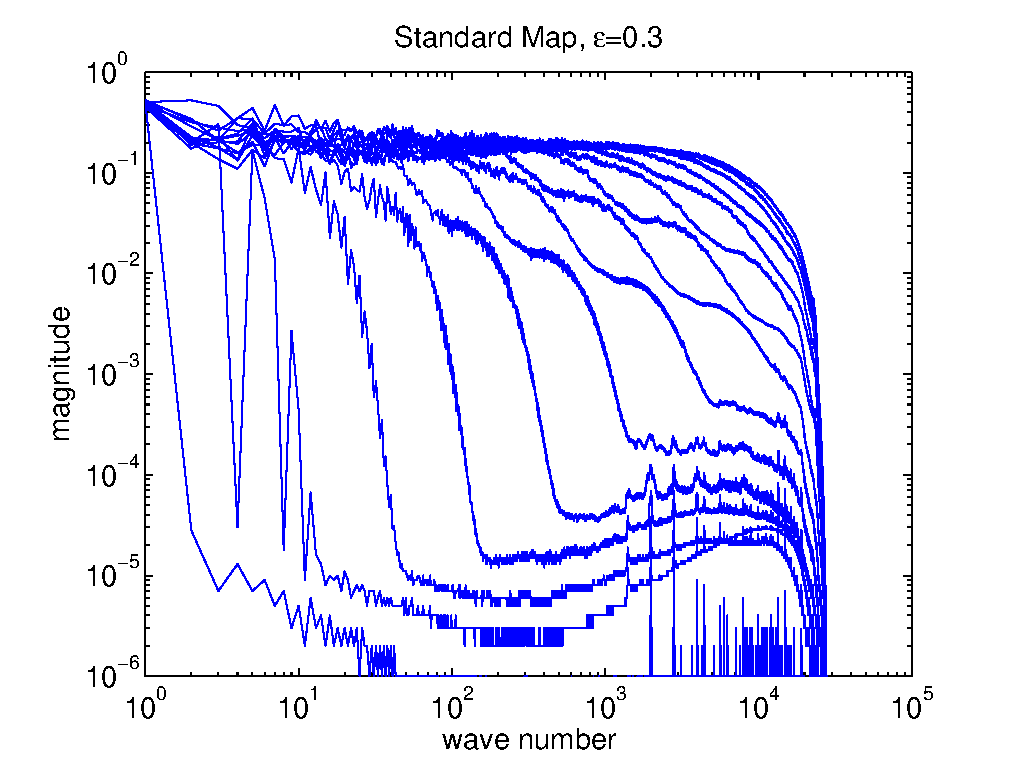
\includegraphics[width=0.5\textwidth]{standardmapfreqevolve}
      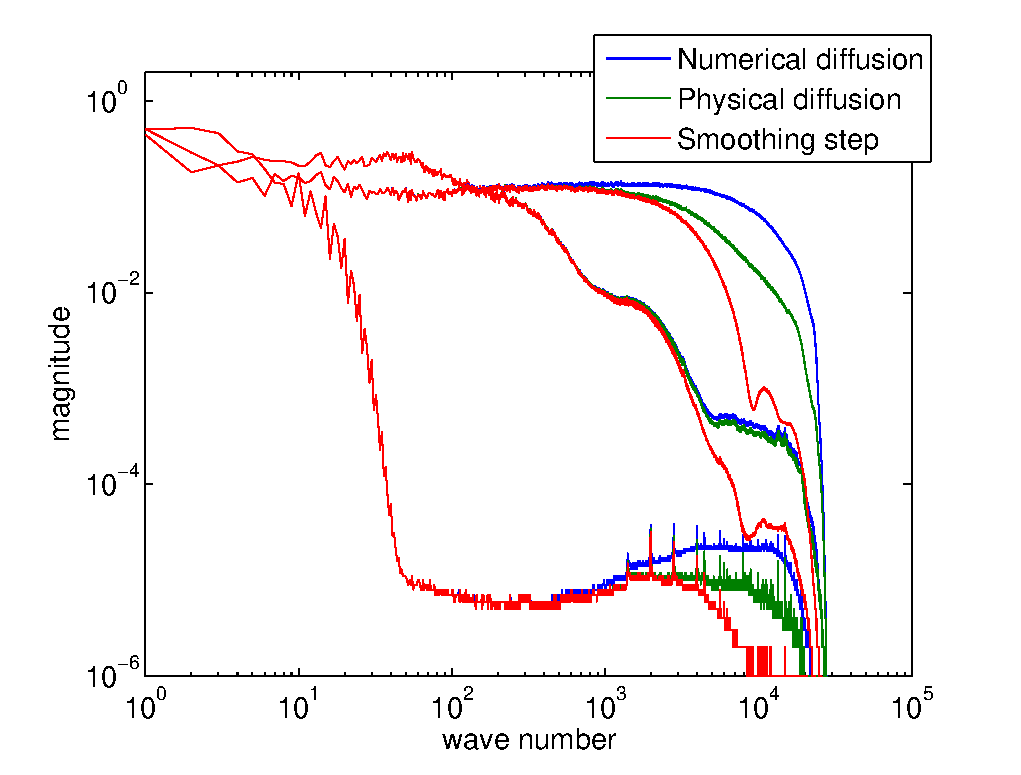
\includegraphics[width=0.5\textwidth]{standardmapfreqcompare}
    }
    \caption{\label{freqcompare}For Standard Map, $\epsilon = 0.3$, $B_n$ with $n=40000^2$ is applied to simulate the system with initial condition $f^0=\cos(2\pi x_2)$. The magnitude versus wave number plot for the first $20$ iterations is shown in the left plot. In the right plot, $B_n$, $\bar{B}_n$, and $\tilde{B}_n$ are applied to simulate the same system and the magnitude versus wave number curves are plotted for iteration $3$, $7$, and $20$.  }
\end{figure}

All three operators $B_n$, $\bar{B}_n$, and $\tilde{B}_n$ satisfying
\begin{eqnarray*}
  \lim_{n \rightarrow \infty} B_n= U_{S^{-1}}, \mbox{  }  \lim_{n \rightarrow \infty} \bar{B}_n= U_{S^{-1}}, \mbox{  }  \lim_{n \rightarrow \infty} \tilde{B}_n=U_{S^{-1}}
 \end{eqnarray*}
can be applied to study the behavior of near-zero diffusion limit of Standard Map. We choose
$B_n$ and $\bar{B}_n$ for the following studies because the computation of FFT/IFFT diffusion of $\tilde{B}_n$ is too expensive when $n$ is very large. Since their relation in the magnitude of diffusion is $B_n<\tilde{B}_n<\bar{B}_n$, if we can show both $B_n$ and $\bar{B}_n$ have similar behaviors, it is reasonable to believe that $\tilde{B}_n$ has, too.

%%%%%%%%%%%%%%%%%%%%%%%%%%%%%%%%%%%%%%%%%%%%%%%%%%%%%%%%%%
\subsection{Cutoff phenomenon}
%%%%%%%%%%%%%%%%%%%%%%%%%%%%%%%%%%%%%%%%%%%%%%%%%%%%%%%%%%


We present the main results of this article in this section. For $n$ from $2500^2$ to $80000^2$, the variance of $f^k_n$ versus iteration plots using $B_n$ and $\bar{B}_n$ as
the Koopman operators are shown in the left of Figures~\ref{standardmapun} and~\ref{smoothingstandardmapun}. The tendency is clear: when $n$ gets larger, the variances stay high ($M_B=M_{\bar{B}}=1$)
for more iterations and then drop rapidly to $m_{B} = 0.4521$ and $m_{\bar{B}}=0.4498$, respectively---they do not drop to zero because there
are unmixed ``islands''. The slope of the rapid dropping also becomes slightly milder when $n$ increases. To
justify whether they satisfy the definition of cutoff given in section~\ref{sec:numcutoffbackground}, we let $t_n$ equal the
point where each trajectory passes through $(M_{\star}+m_{\star})/2$, where $\star=\{B,\bar{B}\}$ and we normalize all trajectories by rescaling
$t_n$ to $1$. The results are plotted in the right of Figure~\ref{standardmapun} and~\ref{smoothingstandardmapun}. Although the normalized trajectories are very similar, one can still
see that when $n$ gets larger, the trajectory becomes sharper. In the left of Figure~\ref{cutofftimeandarea} we plot $t_n$ versus $1/n$ in log scale and see two straight lines. Note that for both cases, we have $D\sim O(1/n)$. Hence this plot shows that the cutoff time is inversely proportional to $\log(D)$. To see how fast the trajectories converge to their limits, we define the interpolating functions for the trajectories in the normalized plots of Figures~\ref{standardmapun} and~\ref{smoothingstandardmapun} to be $\beta_{B_n}(x)$ and $\beta_{\bar{B}_n}(x)$, where $x$ represents the normalized iteration. The function they should converge to when $n\to \infty$ is
\begin{eqnarray}
   \label{limittraj}
   \nu_{\star_\infty}(x) = \begin{cases}
                     M_{\star} &\text{ if } x<1, \\
                     m_{\star} &\text{ otherwise}, \\
                     \end{cases} 
\end{eqnarray}
where $\star=\{B,\bar{B}\}$. Define the distance between $\nu_{\star_n}(x)$ and $\nu_{\star_\infty}(x)$ to be
\begin{eqnarray}
    \label{trajdistance}
    \Delta_{\star}^l= \int_0^l | \nu_{{\star}_\infty}(x)-\nu_{{\star}_n}(x)|dx
\end{eqnarray}
for $\star=\{B,\bar{B}\}$. We calculate $\Delta^3_B$ and $\Delta^3_{\bar{B}}$ for all $\nu_{B_n}(x)$ and $\nu_{\bar{B}_n}(x)$, and plot them versus $t_n$ in the right of Figure~\ref{cutofftimeandarea}. This figure shows that when $t_n$ increases, $\Delta_{\star}^3$ decays slightly slower than linear, but clearly when $n \rightarrow \infty$, $\Delta^3_{B}$ and $\Delta^3_{\bar{B}}$ are both going down, which strongly suggests that both sequences of Markov Chains present cutoffs. 

%$\{B_n, g_n(\cos(2\pi x_2)) \}$ and $\{\bar{B}_n, g_n(\cos(2\pi x_2)) \}$ present cutoffs.

\begin{figure}
    \centerline{
      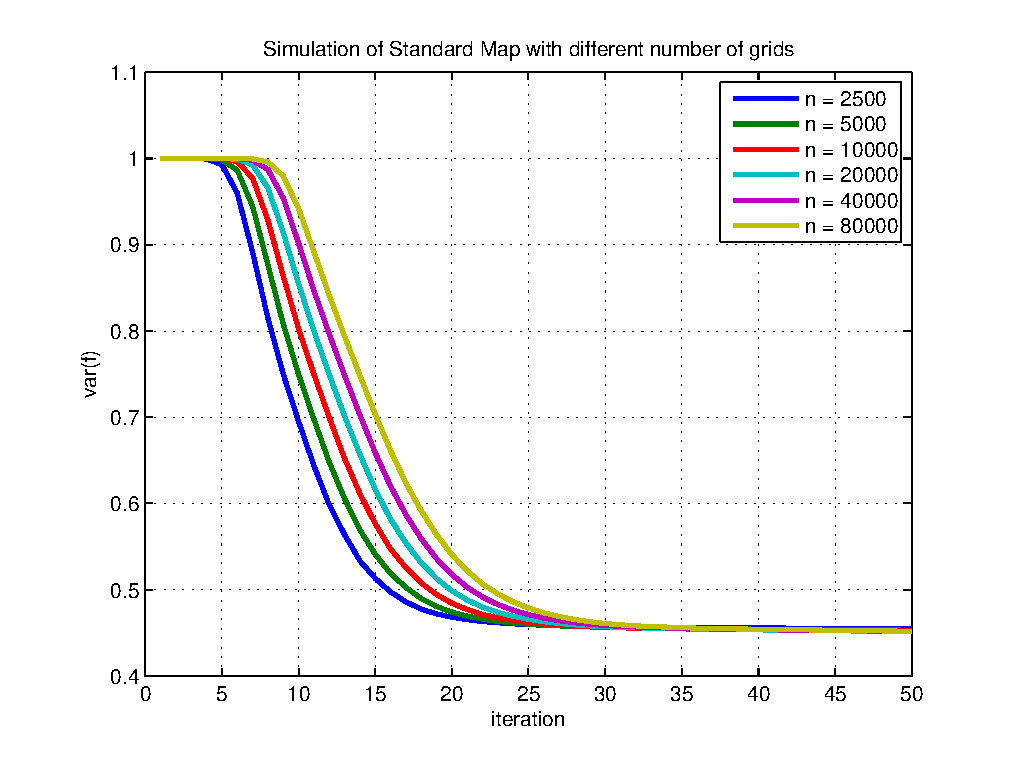
\includegraphics[width=0.5\textwidth]{standardmapcutoff}
      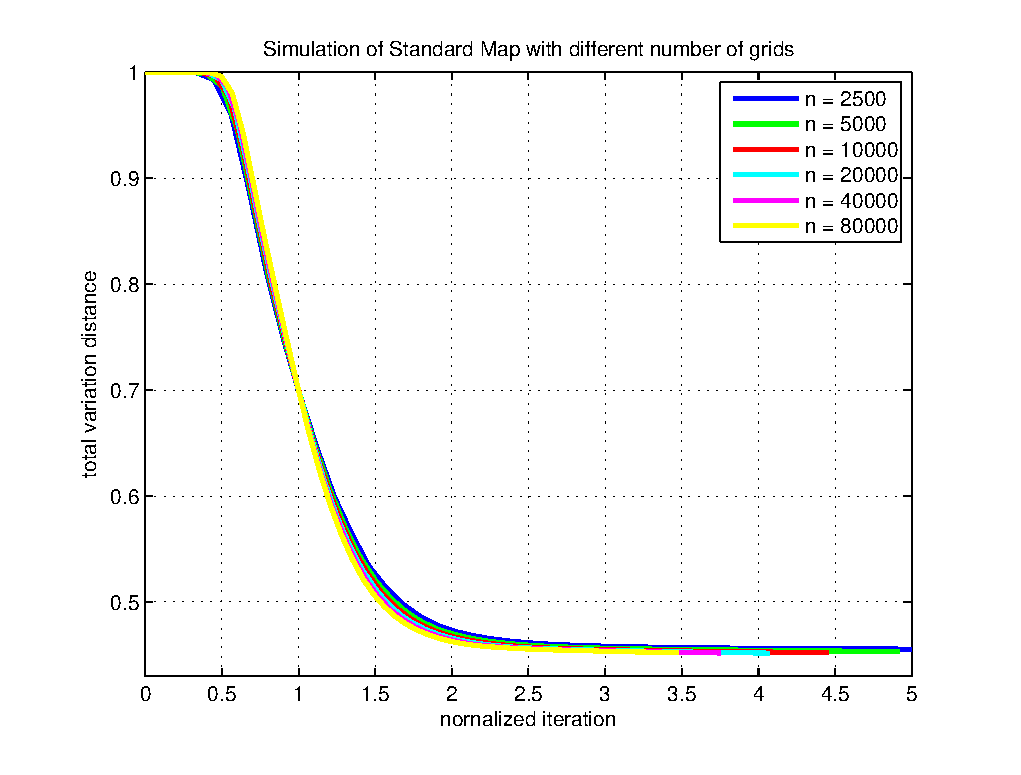
\includegraphics[width=0.5\textwidth]{standardmapcutoffn}
    }
    \caption{The left figure shows the variance of $f_n^k$ versus iteration trajectories of Standard Map simulation. We use $\epsilon=0.3$, $f^0=\cos(2 \pi x_2)$, and number of grids varies from $2500^2$ to $80000^2$. The normalized plot is shown on the right. We rescale the iteration axis and make all trajectories pass through the point $(1,0.7260)$ to observe the cutoff. The two small plots show the detailed view of the corners when trajectories have sharp change.}
 \label{standardmapun}
\end{figure}


\begin{figure}
    \centerline{
      \includegraphics[width=0.5\textwidth]{standardmapcutoffwithsmoothing}
      \includegraphics[width=0.5\textwidth]{standardmapcutoffwithsmoothingn}
    }
     \caption{The left figure shows the variance of $f_n^k$ versus iteration trajectories of Standard Map simulation when a smoothing step is added after each iteration. We use $\epsilon=0.3$, $f^0=\cos(2 \pi x_2)$, and the number of grids varies from $2500^2$ to $80000^2$. The normalized plot is shown in the right. We rescale the iteration axis and make all trajectories pass through the point $(1,0.7249)$ to observe the cutoff. The two small plots show the detailed view of the corners when trajectories have sharp change.}
\label{smoothingstandardmapun}
\end{figure}


\begin{figure}
   \label{cutofftime}
    \centerline{
      \includegraphics[width=0.5\textwidth]{cutofftimevsD}
      \includegraphics[width=0.5\textwidth]{areavscutofftime}
          }
     \caption{\label{cutofftimeandarea} The left plot shows how cutoff time $t_n$ relates to $1/n$ in log scale. Since we have $D \sim O(1/n) $ for our simulation strategy, one can conclude that $t_n$ is inversely proportional to $\log(D)$. The right plot shows how the normalized trajectories converge to their limit. $\Delta^3$ is defined in equation (\ref{trajdistance}). Both curves predict that when $t_n$ is very large, $\Delta^3$ goes down, and the normalized trajectory would probably become a step function.}
\end{figure}
%%%%%%%%%%%%%%%%%%%%%%%%%%%%%%%%%%%%%%%%%%%%%%%%%%%%%%%%%%
\subsection{Chaotic parameter $\epsilon$}
%%%%%%%%%%%%%%%%%%%%%%%%%%%%%%%%%%%%%%%%%%%%%%%%%%%%%%%%%%
We also study how the parameter $\epsilon$ affects the mixing trajectory when the diffusion is small. We use $f^0=\cos(2\pi x_1)$ and $f^0=\cos(2\pi x_2)$ as the initial functions and vary $\epsilon$ from $0.1$ to $0.9$. The simulation is done by $n=40000^2$ with operator $B_n$. The results are shown in Figure~\ref{standardmapparamxy}. For both initial functions and $\epsilon \ge 0.3$, the trajectories all have similar tendency. As for $\epsilon=0.1$, the trajectories show no sign of dropping in the first 50 iterations. Hence in Figure~\ref{standardmapparamsmall} we simulate $\epsilon=0$ and $0.1$ for both initial functions for $800$ iterations. One can see that for $f^0= \cos(2 \pi x_2), \epsilon=0$, the trajectory still stay almost $1$ for the first $800$ iterations, and in the case $\epsilon=0.1$ it has a small drop but we have no evidence to say it presents a cutoff or not. A more interesting thing is observed when $f^0= \cos(2 \pi x_1)$. In this case, the trajectory of $\epsilon=0$ crosses over the one of $\epsilon=0.1$ at around iteration $627$. The phenomenon that the $\epsilon=0$ map mixes faster than some other trajectories with higher $\epsilon$ is also observed in \cite{Mezic2005}. Clearly this is because when $\epsilon=0$, there is no unmixed region (no ``islands'') and so the decreasing rate of variance would not slow down by forming the eigenfunction. Hence when $\epsilon = 0$ the mixing rate only depends on whether the map is good in mixing the initial functions.

\begin{figure}
    \centerline{
      \includegraphics[width=0.5\textwidth]{standardmapparamx}
      \includegraphics[width=0.5\textwidth]{standardmapparamy}
    }
    \caption{\label{standardmapparamxy} The two figures show the Standard Map simulations using $B_n$, $n=40000^2$ with different $\epsilon$ and initial function $f^0$. For $\epsilon=\{0.3,0.5,0.7,0.9 \}$ and $f^0=\{\cos{(2\pi x_1)},\cos{(2\pi x_2)}\}$, the variance trajectories all have sharp changes.}

\end{figure}


\begin{figure}
    \centerline{
      \includegraphics[width=0.5\textwidth]{standardmapparamsmall}
    }
    \caption{\label{standardmapparamsmall} This figure shows the Standard Map simulation with $\epsilon=\{0,0.1\}$ and $f^0=\{\cos{(2\pi x_1)},\cos{(2\pi x_2)}\}$. For $f^0=\cos(2\pi x_2)$, the limiting behavior of $\epsilon \rightarrow 0$ is quite clear. However, for $f^0=\cos(2\pi x_1)$, the $\epsilon=0$ trajectory crosses over the $\epsilon=0.1$ one near iteration $627$.}

\end{figure}

All the numerical results are generated by a 72-node cluster with gigabit ethernet connection. Each CPU is equipped with 1GB RAM, and the largest simulation ($80000\times80000$ number of grids) needs $51.2$GB of memory to store a state vector.



%%%%%%%%%%%%%%%%%%%%%%%%%%%%%%%%%%%%%%%%%%%%%%%%%%%%%%%%%%
\subsection{Zero diffusion and norm issues}
%%%%%%%%%%%%%%%%%%%%%%%%%%%%%%%%%%%%%%%%%%%%%%%%%%%%%%%%%%
In all above simulations we observe how the variance of a scalar function is evolved by Standard Map with small diffusion. As we have mentioned, this is equivalent to the study of $L_2$ cutoff. One may also be interested in how other norms are evolved. In the left plot of Figure~\ref{normcompare} we simulate Standard Map, $\epsilon=0.3$ and $f^0= \cos(2\pi x_1)$ by $B_n$ with $n=500^2$ and measure the following norms: $L_1$, $L_2$, $H_{-0.5}$, $H_{-1}$, and mix-norm \cite{Mezic2005}. All norms are normalized to equal $1$ at iteration $0$. Comparing with previous simulations, this one is done by very coarse grids, so one would not expect to see a very clear cutoff tendency. Nonetheless, these norms do form two groups of different behaviors: for $L_1$ and $L_2$ norms, one observes concave curves in the first few iterations, and for other norms, they drop immediately to around $0.5$ and then oscillate. 


To explain what causes this, let us consider the zero diffusion case: Standard Map is volume preserved, so without diffusion, the $L_1$ norm of the scalar function should stay constant when the function is evolved by the Koopman operator of Standard Map. Also, $L_2$ norm is invariant in the spatial and frequency domain. It is clear that the $L_2$ norm would also stay constant if there is no diffusion. For $H_{-0.5}$, $H_{-1}$, and mix-norm, they have a simple representation in frequency domain. Just the way diffusion works, to evaluate these norms, one multiplies each wave number term by a constant weight, and the weight is decreasing when the wave number increases. For 2-D domain, we plot the weights for each wave number in the right plot of Figure~\ref{normcompare} for all the norms. The diffusion weights when $D=0.01$ is also plotted on the same figure for comparison. One can conclude that the way $H_{-0.5}$, $H_{-1}$, and mix-norm work in frequency domain is very similar to diffusing the function according to a large diffusion and then evaluating their $L_2$ norms: the diffusion is very large ($D \sim 0.01$) and far from entering the region where we can observe cutoffs.  
One important feature of all $2$-D chaotic maps is the frequency cascade: it generates high wave number terms in just a few iterations, as we have seen in Figure~\ref{freqcompare}. The three norms $H_{-0.5}$, $H_{-1}$, and mix-norm suppress these terms by multiplying by small weights. The interesting cutoff phenomenon happens when diffusion is very small: $t_n\sim O(-\log(D))$. Thus these three norms lack the ability to capture things happening in small scales.

Finally we want to stress that there is no one norm that is better than another. They simply give us different information about the mixing process. The concave trajectories of $L_1$ and $L_2$ norms tell us the ``irreversibility'' feature of the chaotic system: beyond a certain iteration, it is not possible to recover the system's original state. The fast dropping trajectories of other norms show the increasing complexity of the function evolved by the chaotic map in the first few iterations.  



\begin{figure}
    \centerline{
      \includegraphics[width=0.5\textwidth]{normcompareplot}
      \includegraphics[width=0.5\textwidth]{normcompareweighting}
    }
    \caption{\label{normcompare} The left figure shows the Standard Map simulation with $\epsilon=0.3$ and $f^0= \cos(2\pi x_1)$. We use $B_n$ with $n=500^2$ and measure the following norms: $L_1$, $L_2$, $H_{-0.5}$, $H_{-1}$, and mix-norm. The norm trajectories form two groups: $L_1$ and $L_2$ norms show the tendency of presenting cutoffs, and the other three norms do not. In the right figure we plot the weights of $L_2$, $H_{-0.5}$, $H_{-1}$, and mix-norm at each wave number in the frequency domain. $L_2$ norm has a constant weight $1$ for all wave numbers. The other three norms have much smaller weights in large wave numbers. We also plot the diffusion weights when $D=0.01$ for comparison. One can see why these norms fail to measure the small-scale phenomena that cause cutoffs.}

\end{figure}




%
% Conclusion
%
\section{Conclusion}
\label{sec:numcutoffconclusion}
In our numerical simulations, we provide the evidence of cutoffs for the sequence of Markov chains generated by approximating the Koopman operator of Standard Map. The notion of a cutoff is first brought from finite Markov Chain studies to the study of chaos, and we find that not only is it suitable for characterizing the behavior of chaotic map in near zero-diffusion limit, but also it builds a bridge between large finite Markov Chain studies and chaotic maps. It is still unclear whether the Markov Chains that present cutoffs have direct link to chaos: are they discretizations or approximations of some chaotic map? We offer no good answer to this question so far. However, in \cite{symdyn} another attempt is made: we show that by choosing suitable initial distributions, a $1$-D chaotic map with symbolic dynamics can have the same limiting behavior as the cutoff of random walk on $n$-dimensional hypercube problem \cite{Diaconis1990}, and thus it demonstrates another link between these two fields.


%%%%%%%%%%%%%%%%%%%%%%%%%%%%%%%%%%%%%%%%%%%%%%%%%%%%%%%%%%
%%%%%%%%%%%%%%%%%%%%%%%%%%%%%%%%%%%%%%%%%%%%%%%%%%%%%%%%%%
\chapter[Cutoffs and Symbolic Dynamics]{Cutoff Phenomenon and the Mixing Property of Chaotic Maps}
%
% Introduction  thesis_chapter_syndyn
%

We relax the definition of the cutoff phenomenon in finite Markov Chains and apply it to the study of the evolution of a probability density function by 1-D chaotic maps. A new object called a stochastic symbol sequence is developed to prove that for a set of initial distributions, the total variation versus iteration curves present cutoffs. Moreover, we can generate a set of initial probability
distributions such that when evolved by chaotic maps, they present the same limit behavior as the cutoff sequences found in specific finite Markov Chains. The results can be applied to any 1-D chaotic map that has full symbolic dynamics.



%How many riffle shuffles are required to sufficiently mix 52 cards? This question have been
%answered by Bayer and Diaconis in \cite{Diaconis1992}. It is quite surprising that the cards are
%highly ordered in the first several shuffles (6 for 52 cards) and then randomized almost abruptly.
%This kind of sharp change in some measure of order/disorder has been discovered in many finite
%Markov Chains, and named cutoff phenomenon \cite{Diaconis1986}. A recent review about the cutoff
%phenomenon of random walks on finite groups can be found in \cite{LSaloff-Costt2004}. On the other
%hand, chaotic mixing process is observed to have similar
%properties \cite{Thiffeault2003-13, Thiffeault2004, Tsang2005}. Think of the cream poured
%into coffee, while stirring, the cream keeps stretching for a while and the mixing with coffee
%happens suddenly. Chaotic mixing has been applied in, for example, microfluidic mixing channel
%design \cite{Ottino2004Science, Wiggins2004, Ottino2004}, random search strategies and
%generating random numbers. However, it is still unclear how to characterize and measure the mixing
%process. In this article, we try to build the relation between cutoff phenomenon and the chaotic
%mixing process by generalizing symbolic dynamics of chaotic maps. The result shows ``cutoff'' in
%the mixing process can be produced by chaotic maps with full symbolic dynamics and certain initial
%conditions.

In the next section, we briefly review cutoff phenomenon and point out how a simple chaotic map can produce ``cutoff''. In section \ref{sec:symdyn} we
introduce symbolic dynamics. We define a new object called stochastic symbol sequence, which serves as the main tool to build the bridge
between cutoff phenomenon and chaotic mixing. The main result is given in section \ref{sec:mainresults}, and finally a conclusion in section \ref{sec:symdynconclusion}.



%
% Body
%
%%%%%%%%%%%%%%%%%%%%%%%%%%%%%%%%%%%%%%%%%%%%%%%%%%%%%%%%%%
%%%%%%%%%%%%%%%%%%%%%%%%%%%%%%%%%%%%%%%%%%%%%%%%%%%%%%%%%%
\section{Background}
\label{sec:background}
%%%%%%%%%%%%%%%%%%%%%%%%%%%%%%%%%%%%%%%%%%%%%%%%%%%%%%%%%%
%%%%%%%%%%%%%%%%%%%%%%%%%%%%%%%%%%%%%%%%%%%%%%%%%%%%%%%%%%

\paragraph{Cutoff phenomenon.} Cutoff phenomenon was discovered by Aldous, Diaconis, and Shahshahani \cite{Diaconis1987, Diaconis1986, Diaconis1981}, and
formalized by Aldous and Diaconis \cite{Diaconis1996, Diaconis1987}. The most interesting cases are found in the random walks on finite
groups with the measure of total variation distance, and most known Markov Chains that present cutoffs can be shown to belong to this
category \cite{LSaloff-Costt2004}. Here we state the definition of a cutoff given by Diaconis in \cite{Diaconis2005}. Assume that to any
finite set $\Omega$ and any pair of probability measures $\omega$, $\bar{\omega}$ on $\Omega$ is associated a real number
$D(\omega,\bar{\omega})$ such that $D(\omega,\bar{\omega})\in [0,1]$,
\begin{eqnarray}
\max_{\Omega,\omega,\bar{\omega}} D(\omega,\bar{\omega}) = 1,
\end{eqnarray}
and $D(\omega,\bar{\omega})=0$ if and only if $\bar{\omega}=\omega$. Consider a sequence of
(finite) probability spaces $(\Omega_n,\bar{\omega}_n)$, $n=1,2,\ldots\ $, each equipped with a sequence
of probability measure $\omega^k_n$, $k=0,1,\ldots\ $, such that
\begin{eqnarray}
\lim_{k \to \infty} D(\omega_n,\bar{\omega}_n)=0.
\end{eqnarray}
The definition of a cutoff follows,

\begin{definition}
\label{cutoffdefinitions} (Diaconis) A family $(\Omega_n,\bar{\omega}_n, (\omega^k_n)_{k=0,1,\ldots})_{n=1,2,\ldots}$ presents a D-cutoff if
there exists a sequence $(t_n)$ of positive reals such that, for any $\epsilon \in(0,1)$,
\begin{enumerate}
  \item $\lim_{n \to \infty}D(\omega^{k_n}_n,\bar{\omega}_n) = 0 \mbox{ if }
  k_n>(1+\epsilon)t_n;$
  \item $\lim_{n \to \infty}D(\omega^{k_n}_n,\bar{\omega}_n) = 1 \mbox{ if }
  k_n<(1-\epsilon)t_n.$
\end{enumerate}
\end{definition}

Cutoff phenomenon is defined for finite Markov Chains and in most cases the Markov transition matrices are generated by symmetric groups.
Since this does not fit our applications in chaotic mixing, we relax the definition and set $\Omega_n$ to be infinite. We say that
a family $(\Omega_n,\bar{\omega}_n, (\omega^k_n)_{k=0,1,\ldots})_{n=1,2,\ldots}$ presents a D-cutoff in the relaxed sense if it satisfies
Definition \ref{cutoffdefinitions} but $\Omega_n$ is infinite. 
%However once the definition is relaxed, the initial distribution is not obvious for each chains and need to be specified.

The distance function we use is the total variation distance.
\begin{definition} For two finite probability distributions $\mu$ and $\nu$, the \textbf{total variation
distance} (TV) between $\mu$ and $\nu$ is
  \begin{eqnarray*}
   |\mu - \nu|_{TV} = \frac{1}{2}\sum_{i} |\mu(i)-\nu(i) |.
  \end{eqnarray*}
\end{definition}
For continuous probability distributions, simply replace the summation by an integration.


The shape of a cutoff can be characterized in several ways \cite{Chen2006}. We are specifically interested in the
``normal'' shape, which is addressed by the following famous cutoff example.

\begin{example} \textbf{Random walk on an $n$-dimensional hypercube} (Diaconis \cite{Diaconis1990})
a particle starts at $\mathbf{0}$ and moves to one of its nearest neighbors (or stay fixed) with equal probability at each step. Let $k =
\frac{1}{4}n\log{n}+cn$. Then for fixed $c \in \mathbb{R}$, as $n \to \infty$,
\begin{eqnarray}
\label{rdwalkshape}
 |\omega^k_n - \bar{\omega} |_{TV} \sim \erf \left(\frac{e^{-2c}}{\sqrt{8}}\right).
\end{eqnarray}
In this example, the cutoff shape is called ``normal'' because of the close relation between normal distribution and error function. In fact, most interesting cutoff examples have normal shapes. When $n \to \infty$ their evolution of total variation distance to uniform can be calculated by evaluating the TV between two normal distributions. This fact becomes crucial in our later discussion. 

\todo{TC: the TV between two normal distributions with the same variance and similar 
means is error function of the difference of their means}





\begin{figure}
\centerline{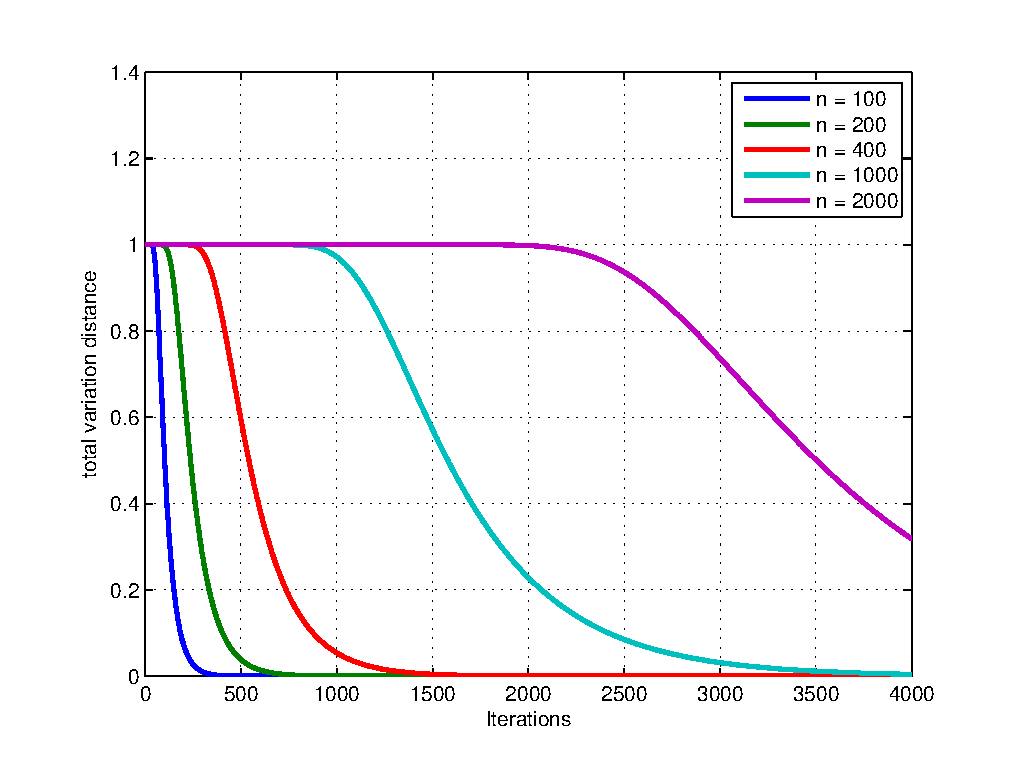
\includegraphics[width=0.7\textwidth,trim=1cm 1cm 0cm 0cm]{rdwalk}} \caption{The $k$
versus $|\omega_n^k-\bar{\omega}|_{TV}$ plot of random walk on an $n$-dimensional hypercube
problem. When $n$ increases, the distance stays close to $1$ for more iterations before it drops to
zero. }
\end{figure}

\end{example}

It is believed that cutoff phenomenon is widespread, although it has been proved only for a small
number of examples. The proof of cutoffs is in general very hard and varies case by case.


Although the study of cutoffs is focused on finite Markov Chains, we care more about what kind of
linear systems can generate convergence trajectories that have sharp changes. It is very hard
to image how a distribution would evolve abruptly to almost uniform from highly
concentrated (in a single state for finite Markov Chains). However, there is an excellent
explanation of why this happens. Consider another famous cutoff example: the Ehrenfest urn problem, involving $2$ urns and $n$
balls. In the beginning all the balls are in urn one, and at each iteration one of the balls is
chosen randomly and put in the other urn. This process is a Markov Chain and it can be shown that
this problem has the same total variation distance $|\omega^k_n-\bar{\omega}|_{TV}$ as the random
walk on hypercubes problem. In fact, this is how people analyze the random walk problem without
actually studying the $2^n$ system states. In this new Markov Chain, there are only $n+1$
states, which stand for the number of balls in urn $2$. In the beginning, all the balls are in urn
$1$ so the probability distribution is concentrated in the first state. The invariant distribution
of this reduced system is a binomial distribution centered at state $(n+1)/2$ (assuming $n$ is odd). By observing how the distribution is evolved when the system iterates, one would see two things:
first, the shape of the distribution gradually becomes binomial to fit the final shape; secondly,
the center of the distribution moves from $0$ toward $(n+1)/2$ at a certain speed (not a constant). When $n$ is large, not only does the center of the
distribution need more iterations to move to $(n+1)/2$, but also the shape of the distribution
needs more iterations to fit the stationary distribution. Cutoff is created by the combination of
these two effects. More details about this explanation can be found in \cite{Lloyd2005}. Now what decides the
shape of the cutoff when $n$ tends to infinity? When $n \to \infty$, a binomial distribution
can be well approximated by a normal distribution. Hence how the total variation distance changes near a
cutoff can be calculated by the TV of two normal distributions, and it has the
form like (\ref{rdwalkshape}). Therefore by forming the reduced system, we see clearly how a cutoff
can happen.





\paragraph{Chaotic Mixing.}
A widely observed phenomenon in the chaotic mixing process when small diffusion exists is the
two- or three-stage transition \cite{Thiffeault2003-13, Fereday2002, Antonsen1996}. The map
does not mix the scalar function with a constant rate in general. When the variance of the scalar
function is measured during the mixing process, one can in general observe a relatively flat decay
followed by a super-exponential change, and then finally it tends to an exponential decay. People
are interested in when these transitions happen, why they happen, and how to predict the slope of
the exponential region. A good review and physical interpretation can be found in
\cite{Thiffeault2004}.

In fact, such multi-stage mixing process can also be found in $1$-D chaotic map when a probability distribution is advected by the Perron-Frobenius operator of the map. To explain this, we first give the definition of the Perron-Frobenius operator \cite{Mezic2005}.

In the measure space $(X,\mathcal{A},\mu)$, for a map $S:X\to X$, we define the following operator. 
\begin{definition} \textbf{ (Perron-Frobenius operator)}
Let $\omega \in L^1(X)$, and suppose that for every $A \in \mathcal{A}$ the operator $P_S:L^1(X) \to L^1(X)$ satisfies
  \begin{eqnarray}
    \int_A P_S \omega(x)\mu(dx) = \int_{S^{-1}(A)} \omega(x)\mu(dx).
  \end{eqnarray}
Then $P_S$ is the Perron-Frobenius operator associated with $S$.
\end{definition}
It tells us how a probability distribution is evolved by a map $S$. 

%%%%%%%%%%%%%%%%%%%%%%%%%%%%%%%%%%%%%%%%%%%%%%
\begin{example} \textbf{Tent map cutoff.}
Consider the tent map
   \begin{eqnarray}
   \label{tentmap}
     x' = S_\text{tent}(x) = 1-2\left|x-\frac{1}{2}\right|
   \end{eqnarray}
with the following initial distributions on $[0 ,1]$:
  \begin{eqnarray}
  \label{tentmapinitial}
    \omega_n^0 = \begin{cases}
                      \frac{1}{\mu_n} &\text{ if } x \le \mu_n,\\
                      0               &\text{ otherwise},
                      \end{cases}
  \end{eqnarray}
where $\mu_1 = 1$, and $\mu_{n+1} = \mu_n/2$. The Perron-Frobenius operator of the tent map is
  \begin{eqnarray}
  \label{tentmapevolve}
    \omega_n^{k+1}(x) = P_\text{tent} \omega_n^{k}(x)
                             = \frac{1}{2}\left( \omega_n^{k}\left(\frac{x}{2}\right)+
                                                 \omega_n^{k}\left(1-\frac{x}{2}\right)  \right).
  \end{eqnarray}
The invariant distribution $\bar{\omega}$ of the tent map is uniform. Let $\nu_n^k =
|\omega_n^k-\bar{\omega} |_{TV}$; we find that
 \begin{eqnarray}
   \nu_n^k =  \begin{cases}
                    1- 2^{1+k-n}  &\text{ if }k \le n-1, \\
                    0             &\text{ otherwise}.
              \end{cases}
 \end{eqnarray}
The trajectories of $\nu_n^k$ with varying $n$ are shown in Figure \ref{tentmapcutoffplot}. It shows a cutoff.
\end{example}
%%%%%%%%%%%%%%%%%%%%%%%%%%%%%%%%%%%%%%%%%%%%%%%%
Hence we give the following simple theorem without proof.
%%%%%%%%%%%%%%%%%%%%%%%%%%%%%%%%%%%%%%%%%%%%%%%%
\begin{theorem} \textbf{(Tent map cutoff)}
\label{tentmapcutoff}
The family $(\Omega,\bar{\omega}, (\omega^k_n)_{k=0,1,\ldots})_{n=1,2,\ldots\,}$, where $\bar{\omega}$ is
uniform in $[0,1]$ and $\omega^k_n$ are defined as in (\ref{tentmapinitial}) and
(\ref{tentmapevolve}), presents a total variation-cutoff in the relaxed sense.
\end{theorem}
%%%%%%%%%%%%%%%%%%%%%%%%%%%%%%%%%%%%%%%%%%%%%%%%
A more general version of the above theorem and its proof can be found in section \ref{sec:mainresults}. Here we simply want to address that with the tent map and a sequence of suitable initial distributions, one can easily generate a sequence of Markov Chains that present a cutoff, though the shape is not normal.

This simple example shows that the tent map can present sharp changes in total variation distance. We would
like to generalize the result to a set of initial distributions and all $1$-D chaotic maps that have
full symbolic dynamics.



\begin{figure}
\centerline{{\includegraphics[width=0.7\textwidth]{tentmapcutoff.eps}}}
\caption{\label{tentmapcutoffplot} The plot of $\nu_n^k$. The trajectories present a cutoff.}
\end{figure}





%%%%%%%%
%%%%%%%%%%%%%%%%%%%%%%%%%%%%%%%%%%%%%%%%%%%%%%%%%%%%%%%%%%
%%%%%%%%%%%%%%%%%%%%%%%%%%%%%%%%%%%%%%%%%%%%%%%%%%%%%%%%%%
\section{Symbolic Dynamics and Stochastic Symbol Sequence}
\label{sec:symdyn}
%%%%%%%%%%%%%%%%%%%%%%%%%%%%%%%%%%%%%%%%%%%%%%%%%%%%%%%%%%
%%%%%%%%%%%%%%%%%%%%%%%%%%%%%%%%%%%%%%%%%%%%%%%%%%%%%%%%%%
%%%%%%%%%%%%%%%%%%%%%%%%%%%%%%
\subsection{Symbolic Dynamics}
%%%%%%%%%%%%%%%%%%%%%%%%%%%%%%
We briefly introduce symbolic dynamics for the study of chaotic maps. We focus on $1$-D chaotic maps, whose symbolic dynamics are semi-infinite sequences. 

Let $\mathcal{S}=\{L, R\}$ be the set of symbols consisting of $L$ and $R$. Define $\Sigma$, the collection of all semi-infinite sequence of elements of $\mathcal{S}$, i.e., $s\in \Sigma$ implies
 \begin{eqnarray}
 s= \{.s_0s_1\cdots s_n\cdots\}
 \end{eqnarray}
with $s_i\in \mathcal{S}$ for all $i$. We refer to $\Sigma$ as the space of semi-infinite sequence of two symbols. We consider a map $\sigma:\Sigma \to \Sigma$, which we shall call the shift map, defined as follows. For $s= \{.s_0s_1\cdots s_n\cdots\}$,
 \begin{eqnarray}
 \sigma(s)= \{.s_1s_2\cdots s_n\cdots\},
 \end{eqnarray}
i.e., the shift operator $\sigma$ simply deletes the first element of the sequence. There are rich results about the relation between symbolic dynamics and chaotic maps. Refer to \cite{Wiggins1990, Holmes1983} for good references. Roughly speaking, one can say that given a chaotic map $S$, on its invariant set $\Lambda$, the function $\phi(x): \Lambda \to \Sigma$, which maps a point in $x\in \Lambda$ to a semi-infinite sequence, is homeomorphism: $S$ acting on $\Lambda$ and $\sigma$ acting on $\Sigma$ are topologically conjugate. In other words, we have the following relation:
 \begin{eqnarray}
 S = \phi^{-1}\circ \sigma \circ \phi.
 \end{eqnarray}
And this explains the ``sensitive to initial condition'' property of chaotic maps.

All the results we derive in the next section in semi-infinite stochastic symbol sequences can be extended to bi-infinite ones without difficulty.

%Let $\mathcal{S}=\{L, R\}$ be the set of symbols consisting of $L$ and $R$. Let $\Sigma$ be the collection of all bi-infinite sequence of elements of $\mathcal{S}$, i.e., $s\in \Sigma$ implies
% \begin{eqnarray}
% s= \{\cdots s_{-n}\cdots s_{-1}.s_0s_1\cdots s_n\cdots\}
% \end{eqnarray}
%with $s_i\in \mathcal{S}$ for all $i$. We will refer to $\Sigma$ as the space of bi-infinite sequence of two symbols. We consider a map $\sigma:\Sigma \to \Sigma$, which we shall call the shift map, defined as follows: for $s= \{\cdots s_{-n}\cdots s_{-1}.s_0\cdots s_n\cdots\}$,
%  \begin{eqnarray}
% \sigma(s)= \{\cdots s_{-n}\cdots s_{-1}s_0.s_1\cdots s_n\cdots\}
% \end{eqnarray}
%$\sigma(\cdot)$ simply shift the dot one digit to the right of the sequence. There are rich results
%about the relation between symbolic dynamics and chaotic maps. Refer to \cite{Wiggins1990, Holmes1983} for good
%references. Roughly speaking, one can say that given a chaotic map $S$, on its invariant set
%$\Lambda$, the function $\phi(x): \Lambda \to \Sigma$, which maps a point in $x\in \Lambda$
%to a bi-infinite sequence, is homeomorphism: $S$ acting on $\Lambda$ and $\sigma$ acting on
%$\Sigma$ are topologically conjugate. In other words, we have the following relation,
% \begin{eqnarray}
% S = \phi^{-1}\circ \sigma \circ \phi
% \end{eqnarray}
%And this explains the ``sensitive to initial condition'' property of chaotic maps.

%In this paper we focus on the study of $1$-D chaotic maps, whose symbolic dynamics are semi-infinite sequences in stead of bi-infinite ones. 

%Define $\hat{\Sigma}$ the collection of all
%semi-infinite sequence of elements of $\mathcal{S}$. Each of the point $x \in \Lambda$ has $s\in
%\hat{\Sigma}$ with the following form,
% \begin{eqnarray}
% s= \{.s_0s_1\cdots s_n\cdots\}
% \end{eqnarray}
%The shift operator $\sigma$ simply deletes the first element of the sequence,
% \begin{eqnarray}
% \sigma(s)= \{.s_1s_2\cdots s_n\cdots\}
% \end{eqnarray}




%%%%%%%%%%%%%%%%%%%%%%%%%%%%%%%%%%%%%%%
\subsection{Stochastic Symbol Sequence}
%%%%%%%%%%%%%%%%%%%%%%%%%%%%%%%%%%%%%%%

Since our goal is to study how the probability density is evolved by the map, and symbolic dynamics
itself does not provide this information, we need a new object called stochastic symbol sequence.

%%%%%%%%%%%%%%%%%%%%%%%%%%%%%%%%%%%%%%%%%%%%%%%%%%%%%%%%%%%%%
% Definition
\begin{definition} \textbf{Stochastic symbol sequence.}
Consider $\mathcal{S}$ to be the symbol list. Let $\Delta$ be the collection of all
semi-infinite sequences of elements in $[0,1]$. We define $\delta^\star \in \Delta$ for each
symbol $\star \in \mathcal{S}$ as
 \begin{align}
 \begin{split}
 \delta^\star &= \{.\delta_0^\star \delta_1^\star\cdots \delta_n^\star\cdots\} \\
 %\delta^R &= \{\cdots \delta_{-n}^R\cdots \delta_{-1}^R.\delta_0^R \delta_1^R\cdots \delta_n^R\cdots\}
 \end{split} 
 \end{align}
with $\delta^\star_i \in [0,1]$ for all $i\ge 0$.
\end{definition}
%%%%%%%%%%%%%%%%%%%%%%%%%%%%%%%%%%%%%%%%%%%%%%%%%%%%%%%%%%%%%


The interpretation of each $\delta_i^\star$ is the probability of $x$ belonging to
symbol $\star$. Let $\Omega\in L^\infty[\Lambda], \int_\Lambda dz=1$ denote the space of
probability distribution in $\Lambda$. For a subspace  $\Lambda_\star \subset \Lambda$ and
$\omega\in \Omega$, we define $\psi^\star: \omega \mapsto \delta^\star$ as
 \begin{eqnarray}
 \label{psidef}
    %\delta^L_i = \int_{\Lambda_L} P^i_S \omega(z)dz \text{,   and  }
    \delta^\star_i = \int_{\Lambda_\star} P^i_S \omega(z)dz \text{, for all }i,
 \end{eqnarray}
where $P_S$ is the Perron-Frobenius operator of map $S$. Denote the $i$-th component of the symbolic dynamics of $x$ as $\phi(x)_i$. The above definition gives a simple relation between the symbolic dynamics and the stochastic symbol sequence. Suppose $x$ has pdf $\omega$, the stochastic symbol sequence of $\omega$ for symbol $\star \in \mathcal{S}$ is $\delta^\star$; then
 \begin{eqnarray}
 \label{deltaistar}
  \delta_i^\star = \prob(\phi(x)_i = \star) \text{, for } \star\in \mathcal{S} \text{ and all }i.
 \end{eqnarray} 

The definition is valid for any number of symbols. However, we only deal with two-symbol cases. For two-symbol cases: $\mathcal{S} = \{L,R\}$ and $\Lambda= \Lambda_L +\Lambda_R  $ , $\delta_i^R$ surely equals $1-\delta_i^L $. For simplicity, we
define $\psi = \psi^L$. We use $\delta$ to denote $\delta^L$ later. However, for clarity, we keep the $L$ for now. 


\begin{example} \textbf{Symbolic representation of the tent map}

Let $\Lambda=[0, 1]$. Partition $\Lambda \cap S^{-1}_{\text{tent}}(\Lambda)$ by writing its two
components as $\Lambda_L$ and $\Lambda_R$. For the tent map, $\Lambda_L=[0, 1/2]$ and $\Lambda_R=(1/2,1]$, we choose $\Lambda_R$ to exclude the point $1/2$ to avoid the overlap. We can associate with
each $x \in \Lambda $ a sequence $s = \{s_i \}_{i=0}^{\infty}$ of $L$'s and $R$'s defined by
$s_i=j$ if $S_{\text{tent}}^i(x) \in \Lambda_j$. The sequence ${s_i}$ labels the iterates of $x$
according to the left-right pattern they follow. In this way, we can label each $x \in \Lambda$
uniquely by a semi-infinite sequence $\phi(x)=s$ where the $s_i$'s are $L$'s and $R$'s. Let
$\Sigma$ denote the space of semi-infinite sequences of two symbols $L$'s and $R$'s. Then
$\phi(x): \Lambda \to \Sigma$ maps a point in $x\in I$ to a semi-infinite sequence.
The shift operator $\sigma$ acts on $s$ by simply dropping the first entry of $s$, i.e.,
$\sigma(\{s_i\}_{i=0}^{\infty})=\{s_i\}_{i=1}^{\infty}$. Similarly the map $\psi: \bar{\Omega}
\to \Delta$, where $\Delta$ denotes the space of semi-infinite stochastic
symbol sequence, maps an $\omega \in \bar{\Omega}$ to semi-infinite stochastic symbol sequences $\{
\delta^L,\delta^R\}$

%Note this is different from how it acts on a bi-infinity sequence, and this demonstrates that the
%tent map ``forgets'' the past information.
%An alternative interpretation of the semi-infinite
%sequence is as follows: one can embed the 1-D map into a 2-D volume preserved map, and make the
%symbol sequence bi-infinite. However, all the $s_i$'s with $i<0$ are unobservable. We can only
%evaluate (and we only care about) the thing happened in the first dimension.
\end{example}

It is clear that the map $\psi: \Omega \to \Delta $, as defined in
(\ref{psidef}), maps a probability distribution $\omega \in \Omega$ to the stochastic symbol
sequence $\delta$ uniquely. Moreover,  we overload the operator $\sigma$ to work
on the space $\Delta$, and have the following lemma.

%%%%%%%%%%%%%%%%%%%%%%%%%%%%%%%%%%%%%%%%%%%%%%%%%%%%%%%%%%%%%
%lemma
\begin{lemma}
  \begin{eqnarray}
 \psi \circ P_S = \sigma \circ \psi.
  \end{eqnarray}
\end{lemma}
\begin{proof} By definition,
  \begin{align}
      \delta_{i+1}^L (\omega)   &= \int_{\Lambda_L} P_S^{i+1} \omega(z)dz \nonumber\\
                                &= \int_{\Lambda_L} P_S^{i} \left(P_S\omega(z) \right) dz \nonumber\\
                                &=  \delta_{i}^L (P_S \omega).
  \end{align}
\end{proof}
%%%%%%%%%%%%%%%%%%%%%%%%%%%%%%%%%%%%%%%%%%%%%%%%%%%%%%%%%%%%%

However, unlike $\phi$, the function $\psi$ is not invertible. There are many $\omega$'s that map to the same $\delta^L$. To resolve this problem, for a given chaotic map $S$ we consider a smaller space:
  \begin{eqnarray}
  \label{DefOmegabar}
  \bar{\Omega} = \left\{ \omega \mid \omega(z) = \lim_{n \to \infty} \prod_{i=0}^n \beta^{\phi(z)_i}_i \right\},
  \end{eqnarray}
where $\beta^L_i \in [0,1]$, $\beta^R_i=1-\beta^L_i$. Remember that $\phi(z)_i$ is the $i$-th component of the symbol sequence of $z$ associated with the chaotic map, so having symbolic dynamics is a necessary condition for having $\bar{\Omega}$.

%%%%%%%%%%%%%%%%%%%%%%%%%%%%%%%%%%%%%%%%%%%%%%%%%%%%%%%%%%%%%
The following lemma justifies the existence of $\psi^{-1}$ in $\bar{\Omega}$.
%lemma
\begin{lemma} For $\omega \in \bar{\Omega}$, one has
 \begin{eqnarray}
    \delta^L_k(\omega) = \beta^L_k(\omega)  \text{, for all }k.
 \end{eqnarray}
\end{lemma}
\begin{proof} By definition,
 \begin{align}
    \delta_{k}^L (\omega)   &= \int_{\Lambda_L} P_S^{k} \omega(z)dz \nonumber\\
                            &= \int_{S^{-k}(\Lambda_L)} \omega(z)dz \nonumber\\
                            &= \lim_{n \to \infty} \sum_{\substack{s\in \Sigma\\s^k= L }}  \prod_{i=0}^{n} \beta^{s_i}_i \nonumber\\
                            &= \beta_k^L \lim_{n \to \infty} \sum_{s\in \Sigma}  \prod_{\substack{i=0\\ i\neq k}}^{n} \beta^{s_i}_i \nonumber\\
                            &= \beta_k^L.
 \end{align}
\end{proof}
%%%%%%%%%%%%%%%%%%%%%%%%%%%%%%%%%%%%%%%%%%%%%%%%%%%%%%%%%%%%%

Hence, in $\bar{\Omega}$ the map $\psi$ is invertible. From now on, the probability space we are interested in is the space $\bar{\Omega}$. It is also easy to check that
 \begin{eqnarray}
 \label{Pconserve}
  P_S (\omega) \in \bar{\Omega}, \mbox{ if } \omega \in \bar{\Omega}.
 \end{eqnarray}
And since $\psi$ is invertible, just like in symbolic dynamics, we also have
 \begin{eqnarray}
 P_S= \psi^{-1}\circ \sigma \circ \psi.
 \end{eqnarray}
It says the Perron-Frobenius operator and the shift operator are conjugate in the spaces $\{\bar{\Omega},\Delta \}$. To understand the special property of the subspace $\bar{\Omega}$, we give the following lemma.

%%%%%%%%%%%%%%%%%%%%%%%%%%%%%%%%%%%%%%%%%%%%%%%%%%%%%%%%%%%%%
%lemma
\begin{lemma} \label{lemma:independency}
For $x \in \Lambda$ having pdf $\omega \in \bar{\Omega}$, and any $s\in \Sigma$, then for any $i,j$, $i\neq j$, 
\begin{equation}
   \phi(x)_i=s_i \mbox{ and } \phi(x)_j=s_j \mbox{ are independent.}
\end{equation}
\end{lemma}
\todo{TC: there might be a better way to state the independence, and need to check is the proof strong enough.}
%one has
% \begin{equation}
%    \prob(\phi(x)_i=s_i) =   \prob(\phi(x)_i=s_i \mid  \phi(x)_k=s_k, k= {0,\ldots,\infty\}, k \neq i )
% \end{equation}
%\end{lemma}

\begin{proof} For $\omega\in \bar{\Omega}$, 
 \begin{align*}
   \prob(\phi(x)=s) &= \lim_{n \to \infty} \prod_{i=0}^{n} \delta_i^{s_i}  \\
                      &=  \lim_{n \to \infty} \prod_{i=0}^{n} \prob(\phi(x)_i=s_i).
 \end{align*}
The second equality is from equation (\ref{deltaistar}). This justifies the claim of independence.   
\end{proof}
%%%%%%%%%%%%%%%%%%%%%%%%%%%%%%%%%%%%%%%%%%%%%%%%%%%%%%%%%%%%%


Furthermore, we define the convex combination of two stochastic symbol sequences to be the convex combination of the individual components and then give another important property of the function $\psi$.
%%%%%%%%%%%%%%%%%%%%%%%%%%%%%%%%%%%%%%%%%%%%%%%%%%%%%%%%%%%%%
%lemma
\begin{lemma}
For any $\omega_1, \omega_2 \in \bar{\Omega}$ and $\alpha\in[0,1]$, one has
 \begin{eqnarray}
 \label{psiislinear}
  \psi(\alpha\omega_1+(1-\alpha)\omega_2) = \alpha\psi(\omega_1)+(1-\alpha)\psi(\omega_2).
 \end{eqnarray}
\end{lemma}

\begin{proof}
  \begin{align}
    \lefteqn{\alpha \delta^L_k(\omega_1) + (1-\alpha) \delta^L_k(\omega_2) } \nonumber\\
                    &=   \alpha \int_{S^{-k}(\Lambda_L)} \omega_1(z)dz+
                          (1-\alpha) \int_{S^{-k}(\Lambda_L)} \omega_2(z)dz \nonumber \\
                    &=   \int_{S^{-k}(\Lambda_L)}\left( \alpha \omega_1(z) +(1-\alpha) \omega_2(z) \right) dz \nonumber \\
                    &=   \delta^L_k( \alpha \omega_1 +(1-\alpha) \omega_2).
  \end{align}
\end{proof}
%%%%%%%%%%%%%%%%%%%%%%%%%%%%%%%%%%%%%%%%%%%%%%%%%%%%%%%%%%%%%
 This property can be extended to the convex combination of $n$ distributions and allows us to prove some important facts later.


We have successfully moved from the probability distribution $\omega \in \bar{\Omega}$ to its
stochastic symbol sequence representation. Now we would like to know how total variation distance
passes through, i.e., given $\omega$ and $\bar{\omega}$ with stochastic symbol sequence
$\{\delta^L, \delta^R\}$ and $\{\bar{\delta}^L,\bar{\delta}^R \}$, respectively, how do we calculate
$|\omega-\bar{\omega}|_{TV}$? The answer is:
 \begin{eqnarray}
 \label{infiniteTV}
|\omega-\bar{\omega}|_{TV} = \frac{1}{2} \lim_{n \to \infty}  \sum_{s\in\Sigma} \left| \prod_{i=0}^n\delta_i^{s_i}-\prod_{i=0}^n\bar{\delta}_i^{s_i}  \right|.
 \end{eqnarray}
This expression is almost impossible to evaluate because of the summation over infinity combinations. So let us consider a simpler case, when $\delta^L$ and $\bar{\delta}^L$ only have $p$ different digits, i.e.,\ $\delta_i^L = \bar{\delta}_i^L$ when $i\notin \theta$, and $|\theta| = p$. Let $\Sigma_p$ be the space of all combinations of $p$ symbol sequence with two symbols. Then we have
 \begin{eqnarray}
  \label{finiteTV}
|\omega-\bar{\omega}|_{TV} = \frac{1}{2} \sum_{s\in\Sigma_p}  \left| \prod_{i\in \theta}\delta_i^{s_i}-\prod_{i\in\theta}\bar{\delta}_i^{s_i}  \right|.
 \end{eqnarray}
In this expression, $s$ is some finite selections of the bi-infinite symbol sequence. The message here is that the total variation distance has nothing to do with the order: it only depends on the elements $s_i, i\in\theta$. Furthermore, (\ref{finiteTV})  can serve as a lower bound when the information besides $i\in \theta$ is unknown.







%%%%%%%%%%%%%%%%%%%%%%%%%%%%%%%%%%%%%%%%%%%%%%%%%%%%%%%%%%
\subsection{General results}
In reality, we may not care about the TV between two probability distributions, but want to know which one of them is closer to the invariant measure of the map. In this section, we give some general results about the TV from a stochastic symbol sequence of two symbols to the distribution $\bar{\omega}$, which has the representation
\begin{equation}
\label{deltabar}
\bar{\delta}=\left\{.\frac{1}{2}\frac{1}{2}\frac{1}{2}\cdots\right\}.
\end{equation}
Clearly (\ref{deltabar}) is invariant under the shift operator, and hence it is an invariant measure of the map. From now on we use $\delta$ to denote $\delta^L$, and if needed, $1-\delta$ represents $\delta^R$. Also, $\delta$ itself without any sub-index represents the whole stochastic symbol sequence, and $\delta_i$ indicates the $i$-th component in $\delta$ on the right-hand side of the dot.

\todo{TC:(\ref{deltabar}) is not the only invariant measure. Any constant sequence is invariant under the shift map, but we are not interested in them.}

The following convexity lemma is the basis of all later results.
%%%%%%%%%%%%%%%%%%%%%%%%%%%%%%%%%%%%%%%%%%%%%%%%%%%%%%%%%%%%%
%lemma
\begin{lemma} For $\delta,\delta^* \in \Delta$, $\alpha\in [0 ,1]$,
 \begin{eqnarray}
\label{convexityofTV}
|\psi^{-1}(\alpha\delta+(1-\alpha)\delta^*)-\bar{\omega}|_{TV} \le
            \alpha|\psi^{-1}(\delta)-\bar{\omega} |_{TV}+(1-\alpha)|\psi^{-1}(\delta^*)-\bar{\omega}|_{TV}.
 \end{eqnarray}
\end{lemma}
\begin{proof}
Since $\omega \mapsto |\omega-\bar{\omega}|_{TV}$ is a convex function, by using
(\ref{psiislinear}) we obtain that the function $\delta \mapsto
|\psi^{-1}(\delta)-\bar{\omega}|_{TV} $ is also convex. The convexity gives us the above
result.
\end{proof}
%%%%%%%%%%%%%%%%%%%%%%%%%%%%%%%%%%%%%%%%%%%%%%%%%%%%%%%%%%%%%



So even if there is no direct way to calculate the TV from a stochastic symbol
sequence to another, we can still use the convexity to deduce some useful bounds.

We give the following lemmas.

%%%%%%%%%%%%%%%%%%%%%%%%%%%%%%%%%%%%%%%%%%%%%%%%%%%%%%%%%%%%%
%lemma
\begin{lemma}
\label{onedifflemma} Suppose $\delta$ and $\delta^*$ are two stochastic symbol sequences corresponding
to the probability distribution $\omega$ and $\omega^*$, respectively. Suppose there exists a
bijection $\gamma: i \mapsto j$ such that $\delta_i = \delta^*_j$ for all $i\in
\mathbb{Z}\setminus\{i^\dagger\}$. If $ |\delta_{i^\dagger}-\frac{1}{2}| \ge |\delta^*_{\gamma(i^\dagger)}-\frac{1}{2}|$, then
 \begin{eqnarray}
      |\omega-\bar{\omega} |_{TV} \ge |\omega^*-\bar{\omega} |_{TV}.
 \end{eqnarray}
\end{lemma}
\begin{proof} Since $|\psi^{-1}(\delta)-\bar{\omega}|_{TV}$ is independent of the order of the sequence, we can assume
$\delta = \delta^*$ for all $i\in \mathbb{Z}\setminus\{i^\dagger\}$. Let $\tilde{\delta} = \delta$
for all $i\in \mathbb{Z}\setminus\{i^\dagger\}$, and
$\tilde{\delta}_{i^\dagger}=1-\delta_{i^\dagger}$. Apparently,
$|\psi^{-1}(\delta)-\bar{\omega}|_{TV} =|\psi^{-1}(\tilde{\delta})-\bar{\omega}|_{TV} $. When
$|\delta_{i^\dagger}-\frac{1}{2}| \ge |\delta^*_{i^\dagger}-\frac{1}{2}|$, it is always possible to
choose $\alpha\in[0,1]$ such that  $\delta^*_i = \alpha \delta_i +(1-\alpha) \tilde{\delta}_i $.
Applying (\ref{convexityofTV}) to $\delta$ and $\tilde{\delta}$ with the $\alpha$ above, we have
\begin{align}
    |\psi^{-1}(\delta^*)-\bar{\omega}|_{TV}
                 &\le  \alpha|\psi^{-1}(\delta)-\bar{\omega} |_{TV}+(1-\alpha)|\psi^{-1}(\tilde{\delta})-\bar{\omega}|_{TV} \nonumber\\
                 & =  |\psi^{-1}(\delta)-\bar{\omega} |_{TV}.
 \end{align}
\end{proof}
%%%%%%%%%%%%%%%%%%%%%%%%%%%%%%%%%%%%%%%%%%%%%%%%%%%%%%%%%%%%%

%%%%%%%%%%%%%%%%%%%%%%%%%%%%%%%%%%%%%%%%%%%%%%%%%%%%%%%%%%%%%
%lemma
\begin{lemma}
\label{alldifflemma} Suppose $\delta$ and $\delta^*$ are two stochastic symbol sequences corresponding
to the probability distribution $\omega$ and $\omega^*$, respectively. Suppose there exists a
bijection $\gamma: i \mapsto j$ such that $|\delta_i-\frac{1}{2}| \ge |\delta^*_j-\frac{1}{2} |$ for
all $i\in \mathbb{Z}$. Then
 \begin{eqnarray}
   |\omega-\bar{\omega} |_{TV} \ge|\omega^*-\bar{\omega} |_{TV}.
 \end{eqnarray}
\end{lemma}
\begin{proof} Apply Lemma \ref{onedifflemma} repeatedly.
\end{proof}
%%%%%%%%%%%%%%%%%%%%%%%%%%%%%%%%%%%%%%%%%%%%%%%%%%%%%%%%%%%%%

The above lemma tells us how to compare $|\omega-\bar{\omega}|_{TV}$ and $|\omega^*-\bar{\omega}|_{TV}$
if some relation of their stochastic symbol sequences is known. Now for a given $\omega$ we want
to bound its $|\omega-\bar{\omega}|_{TV}$ by choosing an $\omega^*$ such that its
$|\omega^*-\bar{\omega}|_{TV}$ is easy to calculate. The choices we made are the sequences with the
following form:
  \begin{align}
  \begin{split}
  \label{deltamM}
   \delta^m &= \{.\underbrace{\delta^m_{\star} \delta^m_{\star} \cdots \delta^m_{\star}}_{p}\frac{1}{2}\frac{1}{2}\cdots \}, \\
   \delta^M &= \{.\underbrace{\delta^M_{\star} \delta^M_{\star} \cdots \delta^M_{\star}}_{p}\frac{1}{2}\frac{1}{2}\cdots \}.
  \end{split}
  \end{align}
As we see later, $|\omega-\bar{\omega}|_{TV}$ can be evaluated easily if $\psi^{-1}(\omega)$ has finite constant leading terms. Note that we use the index $\star$ to indicate that $\delta_{\star}^M$ and $\delta_{\star}^m$ are numbers, not sequences.

  
%Where $\delta^m_0=\delta^m_1= \cdots = \delta^m_{p-1} \equiv \delta^m_{\star}$ and
%$\delta^M_0=\delta^M_1= \cdots = \delta^M_{p-1}\equiv \delta^M_{\star}$.


%First we are going to generalize the lower bound result from $\delta_i=1$, for $i\in \theta$ to $\delta_i=\delta^M$. Note here $\delta^M$ is a number, $1/2 \le \delta^M \le 1$.

%%%%%%%%%%%%%%%%%%%%%%%%%%%%
\subsubsection{Lower Bound}
%%%%%%%%%%%%%%%%%%%%%%%%%%%%%

%%%%%%%%%%%%%%%%%%%%%%%%%%%%%%%%%%%%%%%%%%%%%%%%%%%%%%%%%%%%%
%theorem
\begin{theorem}
\label{theoremlb} Suppose $\delta$ and $\bar{\delta}$ are two stochastic symbol sequences corresponding
to the probability distribution $\omega$ and the invariant distribution $\bar{\omega}$,
respectively. Suppose there is a set $\theta \subset \mathbb{Z}^++\{0\} $, $|\theta|=p$ such that
for all $i \in \theta$, $|\delta_i-\frac{1}{2}|>|\delta^m_\star-\frac{1}{2}|$. Then
\begin{eqnarray}
\label{lbineq}
|\omega-\bar{\omega}|_{TV} \ge \mathbf{I}_{\frac{1}{2}}(p-q^*,q^*+1) - \mathbf{I}_{1-\delta^m_\star}(p-q^*,q^*+1),
\end{eqnarray}
where
\begin{eqnarray}
\label{kstar}
q^* =  \left\lfloor p \frac{\log{2}+\log{(\frac{1}{2}-\epsilon)} }{\log{(\frac{1}{2}-\epsilon)}-\log{(\frac{1}{2}+\epsilon})} \right\rfloor,
\end{eqnarray}
$\epsilon = |\delta^m_\star-\frac{1}{2}|$, and $\mathbf{I}$ is the regularized incomplete
beta function.
\end{theorem}
\begin{proof}
Since the TV is independent of the order of the sequence, we can assume that
$\theta=\{0,1,\ldots,p-1\}$. Also, without loss of generality, we assume for $i\in \theta$,
$\delta_i \ge \epsilon+\frac{1}{2}= \delta^m_\star$. Using equation (\ref{finiteTV}) and Lemma
\ref{alldifflemma}, we have
\begin{align}
\label{lbtv}
|\omega-\bar{\omega}|_{TV}
                      &\ge \frac{1}{2} \sum_{s\in\Sigma_p}
                             \left| \prod_{i\in \theta}\delta_i^{s_i}-\prod_{i\in\theta}\bar{\delta}_i^{s_i}  \right| \nonumber\\
                      &\ge \frac{1}{2}  \sum_{q=0}^{p}
                             {p \choose q} \left|(\delta^m_\star)^q (1-\delta^m_\star)^{p-q} - \frac{1}{2^p} \right| \nonumber \\
                      &=   \frac{1}{2}  \sum_{q=0}^{p} \left|{p \choose q} (\delta^m_\star)^q (1-\delta^m_\star)^{p-q} -{p \choose q} \frac{1}{2^p} \right|.
\end{align}
\end{proof}
\todo{TC: The first line is an inequality because $p < \infty$. }

%%%%%%%%%%%%%%%%%%%%%%%%%%%%%%%%%%%%%%%%%%%%%%%%%%%%%%%%%%%%%

So the total variation distance can be lower bounded by the difference between two binomial
distributions. We can find their difference by subtracting their cumulative distribution functions
at the point they cross over each other. To do this we needs to find the point where the first
distribution begins to exceed the second distribution, which is to find the largest $q^*$ such that
\begin{eqnarray}
\left(\frac{1}{2}+\epsilon\right)^{q^*}\left(\frac{1}{2}-\epsilon\right)^{p-1-q^*}-2^{-p} \le 0.
\end{eqnarray}
Solving for $q^*$ gives (\ref{kstar}), and the cdf of a binomial distribution can be expressed in terms
of the regularized incomplete beta function $\mathbf{I}$ as follows. For the distribution
$\text{binomial}(r,p)$, its cdf is
\begin{eqnarray}
   F(q;p,r) = \mathbf{I}_{1-r}(p-q,q+1).
\end{eqnarray}
Substituting $q^*$ into $q$, and $1/2$ and $\delta^m_\star$ into $r$, we get (\ref{lbineq}).
%\begin{eqnarray}
%|\omega-\bar{\omega}|_{TV} \ge \mathbf{I}_{\frac{1}{2}}(p-k^*,k^*+1) - \mathbf{I}_{1-\delta^m}(p-k^*,k^*+1)
%\end{eqnarray}


An interesting corollary is that when $p$ goes to $\infty$, $|\omega-\bar{\omega}|_{TV}$ goes
to $1$ for all $\epsilon>0$. So each of the constant stochastic symbol sequences actually
represents an eigenfunction or an invariant measure of the map with eigenvalue $1$.




%%%%%%%%%%%%%%%%%%%%%%%%%%%
\subsubsection{Upper Bound}
%%%%%%%%%%%%%%%%%%%%%%%%%%%

We have seen that for a constant sequence with components not equal to $1/2$, the total variation
distance to the invariant distribution $\bar{\omega}$ is $1$ from the previous theorem. Hence this
result does not give us any information about the upper bound. We would like to bound the distance
by the sum of the sequence, and give the following theorem.
\begin{theorem}
\label{theoremub}Suppose $\delta$ and $\bar{\delta}$ are two stochastic symbol sequences corresponding
to the probability distribution $\omega$ and the invariant distribution $\bar{\omega}$,
respectively. Suppose $\sum_{i=0}^\infty |\delta_i - \frac{1}{2}| = \frac{M}{2}$. Then
\begin{eqnarray}
|\omega-\bar{\omega}|_{TV} \le  \begin{cases}
                                   \rho - 2^{-\lceil M \rceil } &\text{ if } \rho>1-2^{-\lceil M \rceil },\\
                                    1-2^{-\lfloor M \rfloor}    &\text{ otherwise},                                   \\
                                \end{cases} 
\end{eqnarray}
where $\rho = \frac{1}{2} +  \frac{M-\lfloor M \rfloor}{2}$.
\end{theorem}
\begin{proof}
With the convexity inequality (\ref{convexityofTV}), one can show that for a set of stochastic symbol sequence $\delta^j$, $j=\{1,2,\ldots\}$, $\sum_j{\alpha_j} = 1$,
\begin{eqnarray}
 \sum_j \alpha_j|\psi^{-1}(\delta^j)-\bar{\omega}|_{TV} \ge |\psi^{-1}(\sum_j \alpha_j \delta^j)-\bar{\omega}|_{TV}.
\end{eqnarray}
So for each $M$, if we can express $\delta$ as the convex combination of a set of $\delta^j$, the total variation distance $|\omega-\bar{\omega}|_{TV}$ can be bounded by the TV of individual $\delta^j$. Let the set $\mathbf{C} = \{\delta \, | \,\sum_i|\delta_i-\frac{1}{2}|  =  \frac{M}{2}\}$. It is easy to see that $\mathbf{C} = \mathbf{conv} \mathbf{D}$, where $\mathbf{D}$ is defined as
\begin{eqnarray}
  \mathbf{D}=\{\delta \mid \delta \text{ has } \lfloor M \rfloor \text{ } 1\text{'s, one } M-\lfloor M \rfloor
               \text{, and all other }\delta_i\text{'s are }\frac{1}{2}  \},
\end{eqnarray}
and $|\psi^{-1}(\delta)-\bar{\omega}(x)|_{TV}$ for each $\delta \in  \mathbf{D}$ can be calculated as
\begin{eqnarray}
|\psi^{-1}(\delta)-\bar{\omega}(x)|_{TV} = 
          \begin{cases}
             \rho - 2^{-\lceil M \rceil } &\text{ if } \rho>1-2^{-\lceil M \rceil },\\
             1-2^{-\lfloor M \rfloor}    &\text{ otherwise},                                   
          \end{cases}
\end{eqnarray}
where $\rho = \frac{1}{2} +  \frac{M-\lfloor M \rfloor}{2}$. We obtain the upper bound by choosing the set of $\delta^j$ to be $\mathbf{D}$.
\end{proof}

Unfortunately, the above upper bound is in general not very tight. We state it just to inspire the next theorem, which gives a tighter bound.
%%%%%%%%%%%%%%%%%%%%%%%%%%%%%%%%%%%%%%%%%%%%%%%%%%%%%%%%%%%%%%%%%%%%%%%%%%%%%%%%%%%%%%%%

\begin{theorem}
\label{theoremub2}
Suppose $\delta$ and $\bar{\delta}$ are two stochastic symbol sequences corresponding to the probability distribution $\omega$ and the invariant distribution $\bar{\omega}$, respectively. Suppose $\sum_{i=0}^\infty |\delta_i - \frac{1}{2}| = \frac{M}{2}$, and $\delta_i \le \delta^M_\star$ for all $i$. Then
\begin{eqnarray}
\label{ubineq}
|\omega-\bar{\omega}|_{TV} \le  \mathbf{I}_{\frac{1}{2}}(p-q^*,q^*+1) - \mathbf{I}_{1-\delta^M_\star}(p-q^*,q^*+1)
\end{eqnarray}
with
\begin{eqnarray}
\label{kstarub}
q^* =  \left\lfloor p \frac{\log{2}+\log{(\frac{1}{2}-\epsilon)} }{\log{(\frac{1}{2}-\epsilon)}-\log{(\frac{1}{2}+\epsilon})}  \right\rfloor,
\end{eqnarray}
where $\epsilon = |\delta^M_\star - \frac{1}{2}|$ and $p = \lceil \frac{M}{2\epsilon}\ \rceil$.
\end{theorem}

\begin{proof} Similarly to the previous proof, let
\begin{eqnarray}
  \mathbf{D}=\{\delta \mid \delta \text{ has } (p-1)\text{ }  of \text{ } \delta^M_\star\text{'s, one } M-(p-1) \delta^M_\star
                \text{, and all other }\delta_i\text{'s are }\frac{1}{2}   \}.
\end{eqnarray}
Then the set  $\mathbf{C} = \{\delta \mid \sum_i|\delta_i-\frac{1}{2}|  =  \frac{M}{2}\}$ satisfies $\mathbf{C} = \mathbf{conv} \mathbf{D}$. All $\delta \in \mathbf{D}$ have the same $|\psi^{-1}(\delta) - \bar{\omega}|_{TV} $ and are bounded by
\begin{eqnarray}
\label{middleineq}
 |\psi^{-1}(\delta) - \bar{\omega}|_{TV} < |\psi^{-1}(\delta^M) - \bar{\omega}|_{TV},
\end{eqnarray}
and $|\psi^{-1}(\delta^M) - \bar{\omega}|_{TV}$ can be calculated similarly to the lower bound proof by finding the $q^*$ such that the first binomial distribution is less than the second one, i.e., find the smallest $q^*$ such that
\begin{eqnarray}
\left(\frac{1}{2}+\epsilon\right)^{q^*}\left(\frac{1}{2}-\epsilon\right)^{p-q^*}-2^{-p} \ge 0.
\end{eqnarray}
Once $q^*$ is solved as in (\ref{kstarub}), we have $|\psi^{-1}(\delta^M) - \bar{\omega}|_{TV} = \mathbf{I}_{\frac{1}{2}}(p-q^*,q^*+1) - \mathbf{I}_{1-\delta^M_\star}(p-q^*,q^*+1)$. Combining with (\ref{middleineq}), one gets (\ref{ubineq}).
\end{proof}



%%%%%%%%%%%%%%%%%%%%%%%%%%%%%%%%%%%%%%%%%
% approximated lower and upper bound
%%%%%%%%%%%%%%%%%%%%%%%%%%%%%%%%%%%%%%%%%
The above lower and upper bound theorems can be applied to any given stochastic symbol sequence as long as one can find $\delta^m$ and $\delta^M$ to bound it. In the following theorem, we consider a scenario that $p \to \infty$ and
$\delta^m_\star (\text{or } \delta^M_\star)\to 1/2$ and calculate where the lower and upper bounds converges to.

%%%%%%%%%%%%%%%%%%%%%%%%%%%%%%%%%%%%%%%%%%%%%%%%%%%%%%%%%
\begin{theorem}
\label{theoremapproxlb} Suppose $\bar{\omega}$ and $\omega_{lb}$ (resp.\ $\omega_{ub}$) are two probability distributions with stochastic symbol sequences $\bar{\delta}$ and $\delta^m$ (resp.\ $\delta^M$) as defined in (\ref{deltabar}) and (\ref{deltamM}), respectively. If $p
\to \infty$ and $\delta^m_{\star}$ (resp.\ $\delta^M_{\star}$)$ \to \frac{1}{2}$, then one has
\begin{align}
\begin{split}
  \label{lbublimit}
                 |\omega_{lb}-\bar{\omega}|_{TV}
               & =  \erf \left( \sqrt{\frac{p}{2}}\left((\delta_{\star}^m)-\frac{1}{2}\right)\right), \\
  \text{resp. }  |\omega_{ub}-\bar{\omega}|_{TV}
               & =  \erf \left( \sqrt{\frac{p}{2}}\left((\delta_{\star}^M)-\frac{1}{2}\right)\right).
\end{split}
\end{align}


\end{theorem}
\begin{proof}
When $p\to \infty$ the binomial distribution approaches the normal distribution as $\text{binomial}\ (\delta^m_{\star},p) \to \mathcal{N}(p\delta^m_{\star}, p\delta^m_{\star}(1-\delta^m_{\star}))$.  The term $|\omega_{lb}-\bar{\omega}|_{TV}$ thus equals the TV between two normal distributions, which can be evaluated by subtracting their cdfs: %Let $(\omega^m)^k \equiv \psi^{-1}(\sigma^k(\delta^M)) $
\begin{align}
  |\omega_{lb}-\bar{\omega}|_{TV}
              &=  \frac{1}{2}\left(1+\erf\left(\frac{x^*-p\delta_{\star}^m}{\sqrt{2p\delta_{\star}^m(1-\delta_{\star}^m)}}\right)\right)
                       -\frac{1}{2}\left(1+\erf\left(\frac{x^*-p\frac{1}{2}}{\sqrt{2p\frac{1}{2}(1-\frac{1}{2})}}\right)\right) \nonumber\\
              &=\erf\left(\frac{x^*-p\delta_{\star}^m}{\sqrt{2p\delta_{\star}^m(1-\delta_{\star}^m)}}\right)-
                       \erf\left(\frac{x^*-p\frac{1}{2}}{\sqrt{2p\frac{1}{2}(1-\frac{1}{2})}}\right),
\end{align}
where $x^*$ is the point the two pdfs crosses over each other. When $\delta_{\star}^m \to \frac{1}{2}$, the denominators in both
$\erf(\cdot)$ are the same, and hence the variances of the two normal distributions are the same while the means differ by
$p(\delta^m_{\star}-\frac{1}{2})$, and one gets (\ref{lbublimit}). Same for the $\omega_{ub}$ equality.

\end{proof}




%Just like the lower bound, we can also give an approximate upper bound,
%\begin{theorem}
%\label{theoremapproxub}  $\delta$ and $\bar{\delta}$ are two stochastic symbol sequences, each
%corresponds to the probability distribution $\omega$ and the invariant distribution $\bar{\omega}$,
%respectively. Suppose $\sum_{i=0}^\infty |\delta_i - \frac{1}{2}| = \frac{M}{2}$, and $p$ is large
%and $\delta^M_\star$ close to $\frac{1}{2}$, then
%\begin{eqnarray}
%\label{lbineqapprox}
%    |\omega-\bar{\omega}|_{TV}   \le  \erf\left( \sqrt{p}\left((\delta_{\star}^M)-\frac{1}{2}\right)\right)
%\end{eqnarray}


%\end{theorem}
%\paragraph{proof} Similar to theorem \ref{theoremapproxlb}




%%%%%%%%%%%%%%%%%%%%%%%%%%%%%%%%%%%%%%%%%%%%%%%%%%%%%%%%%%
%%%%%%%%%%%%%%%%%%%%%%%%%%%%%%%%%%%%%%%%%%%%%%%%%%%%%%%%%%
\section{Main results}
\label{sec:mainresults}
%%%%%%%%%%%%%%%%%%%%%%%%%%%%%%%%%%%%%%%%%%%%%%%%%%%%%%%%%%
%%%%%%%%%%%%%%%%%%%%%%%%%%%%%%%%%%%%%%%%%%%%%%%%%%%%%%%%%%
In the previous section we only deal with the relation between given $\omega$ and $\bar{\omega}$, and there is no evolution. In this section we talk about how to use the results we have to bound $|\omega^k-\bar{\omega}|_{TV}$ when the system iterates with $k$. In general it is no easier to find the stochastic symbol sequence of a probability distribution than to evolve it by the chaotic map directly. Therefore the upper and lower bounds are not practically applicable to tell us the shape of the convergence trajectory for a given initial distribution. Nonetheless, they do provide us a way to observe what creates the sharp change in the total variation distances: the moving and reshaping of a binomial (or binomial-like) distribution to another. Here we consider two interesting examples, where given the stochastic symbol sequences of some functions, we can observe how their $|\omega^k-\bar{\omega}|_{TV}$ change.

\begin{example}
\label{example:constantoega0}
Suppose $\omega^0$ has stochastic symbol sequence as follows:
  \begin{eqnarray}
  \label{constantomega0}
   \psi(\omega^0) =  \{.\underbrace{\delta_\star \delta_\star \cdots \delta_\star}_{p}\frac{1}{2}\frac{1}{2}\cdots\},
  \end{eqnarray}
and $\delta_\star >\frac{1}{2}$. This choice of $\delta$ is the same as in (\ref{deltamM}). Now we want to observe how $|\omega^k-\bar{\omega} |_{TV}$ evolves with $k$. As we have mentioned before, when $p \to \infty$, $|\omega^k-\bar{\omega}|_{TV} = 1$ for any $k>0$, so that is not the case we are interested in. We set $p$ to be a finite number and it is then obvious that $|\omega^p-\bar{\omega}|_{TV} = 0$. However, how sharp is the change from the initial distance to zero? This depends both on $p$ and $\delta_\star$. We plot the $|\omega^0-\bar{\omega} |_{TV}$ versus $p$ trajectories for $\delta_\star=\{0.6, 0.7,0.8,0.9\}$ in the right plot of Figure \ref{deltaMexample1}. Note that one can also view these figures as $|\omega^k-\bar{\omega}|_{TV}$ versus $k$ with fixed $p=300$ for $\psi(\omega^0)$, because the shift operator takes out one $\delta_\star$ per iteration.

When $\delta_\star=1$, the trajectory is already shown in Figure \ref{tentmapcutoffplot}. Now from this figure we know that even when $\delta_\star$ is smaller than $1$, we still see the concave sharp change before TV goes to zero. 

An easier way to see why the concave trajectories occur is to plot the distributions $\omega$ and $\bar{\omega}$ in a reduced space. We know
 \begin{align}
  |\omega-\bar{\omega}|_{TV}
       &= \frac{1}{2} \sum_{s\in\Sigma_{p}}
         \left| \prod_{i=0}^p\delta_i^{s_i}-\prod_{i=0}^p\bar{\delta}_i^{s_i}  \right| \nonumber\\
       &= \frac{1}{2}  \sum_{q=0}^p
          {p \choose q} \left|(\delta_\star)^q (1-\delta_\star)^{p-q} - \frac{1}{2^p} \right| \nonumber \\
       &=  \frac{1}{2}  \sum_{q=0}^p \left|{p \choose q} (\delta_\star)^q (1-\delta_\star)^{p-q} -{p \choose q} \frac{1}{2^p} \right|.
 \end{align}
We can plot the two terms ${p \choose q} (\delta_\star)^q (1-\delta_\star)^{p-q}$ and ${p \choose q} \frac{1}{2^p}$ using $p/q$ as the horizontal axis, to observe their overlap. Suppose we fix $\delta_\star = 0.7$ and vary $p$. In the left plot of Figure \ref{deltaMexample1}, when $p$ is small, the binomial distributions of $(\delta_\star,p)$ and $(\frac{1}{2},p)$ have more overlap, and we clearly see what causes the drop in TV.

\todo{TC: correct the x-axis in Figure \ref{deltaMexample1} from $i$ to $p$, and what is the y-axis?}
\todo{TC: In the right plot of Figure \ref{deltaMexample1}, the legend is $\delta_\star$ not $\delta^M$. }

\begin{figure}
\centerline{{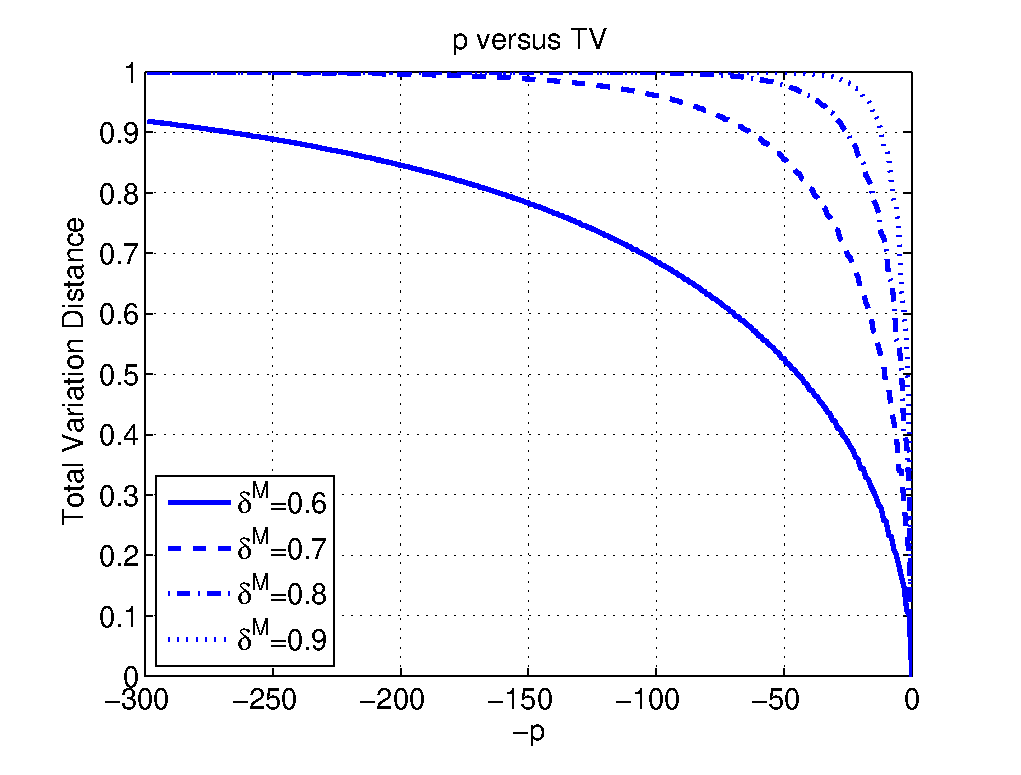
\includegraphics[width=0.5\textwidth]{deltaMexample1a}}
            {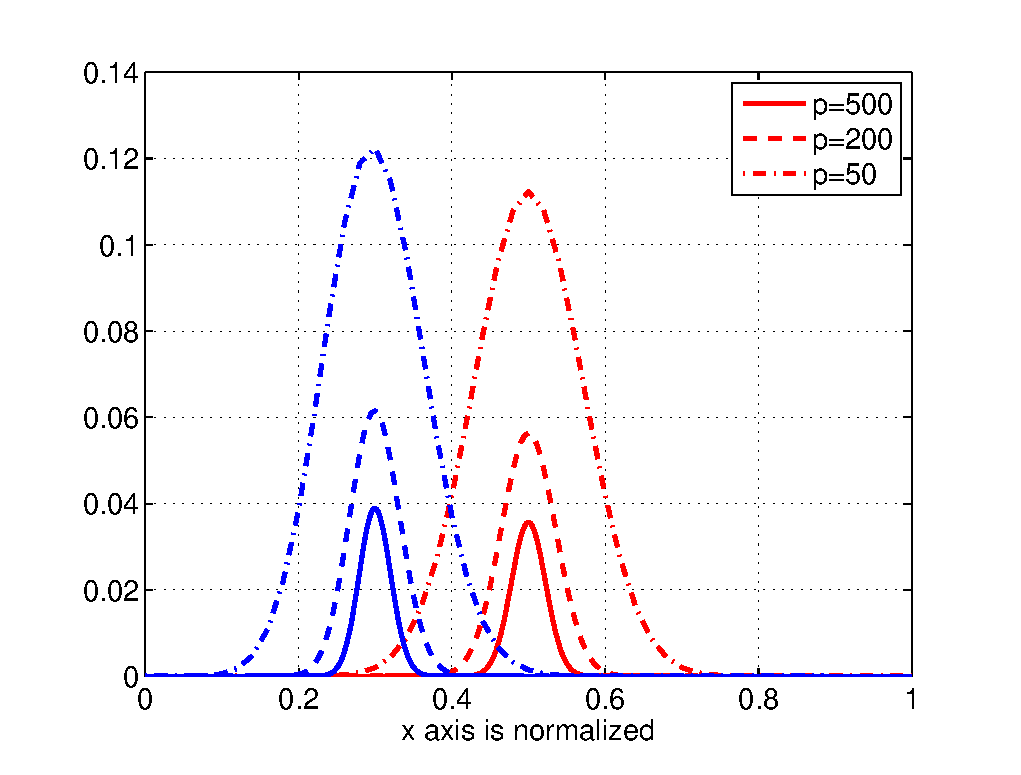
\includegraphics[width=0.5\textwidth]{deltaMexample1b}}}
\caption{\label{deltaMexample1}The left figure shows how one can evaluate
$|\omega^0-\bar{\omega}|_{TV}$, where $\omega^0$ has the form in equation (\ref{constantomega0}),
by finding the overlap area of two binomial distributions centered at $p\delta_\star^a$ and $p/2$.
When $p$ is large, the overlap area gets smaller. The right figure shows how
$|\omega^0-\bar{\omega}|_{TV}$ changes with $p$ for different $\delta_\star$'s. Since evolving
the distribution (\ref{constantomega0}) is equivalent to change $p$, this set of trajectories can
be also interpreted as $|\omega^k-\bar{\omega}|_{TV}$ for $k=300-p$}.
\end{figure}

\end{example}
From the above example, we can give the following theorem.
\begin{theorem}
For a $1$-D map $S:\Lambda \to \Lambda$ having symbolic dynamics, the family \\$(\Omega,\bar{\omega},(\omega^k_n)_{k=0,1,\ldots})_{n=1,2,\ldots}$ presents a total variation-cutoff in the relaxed sense, where
\begin{equation*} 
 \psi(\omega^0_n) =  \{.\underbrace{\delta_\star \delta_\star \cdots \delta_\star}_{n}\frac{1}{2}\frac{1}{2}\cdots\} 
\end{equation*}
for $\omega^0_n\in\bar{\Omega}$ and $0 \le \delta_\star \le 1$. 
\end{theorem}
\begin{proof}
Let $t_n = n$, when $k_n>(1+\epsilon)n$, $|\omega^k_n-\bar{\omega}|_{TV}=0$. When $k_n<(1-\epsilon)n$, $n-k_n>\epsilon n$, and 
\begin{align*}
      |\omega_n^{k_n}-\bar{\omega}|_{TV} &   = |\omega_n^{n-{(n-{k_n})}}-\bar{\omega}|_{TV} \\
                                         & \ge |\omega_n^{n-{\lceil\epsilon n \rceil}}-\bar{\omega}|_{TV}\\
                                         &   = |\omega_p^{{p-{\lceil\epsilon n \rceil}}}-\bar{\omega}|_{TV}  \text{ for any } p\ge n \\
                                         &\to 1 \text{ when } n \to \infty.
\end{align*}
\end{proof}

Theorem \ref{tentmapcutoff} is a special case of the above theorem with $\delta_\star = 1$. 



%%%%%%%%%%%%%%%%%%%%%%%%%%%%%%%%%%%%%%%%%%%%%%%%%%%%%%%%%%%%%%%%%%%%%%%%%%%%%%%%%%
\begin{example}
Suppose $\omega^0$ has stochastic symbol sequence as follows:
  \begin{eqnarray}
  \label{expw0}
   \psi(\omega^0) =  \{.\delta_0 \delta_1 \delta_2 \cdots\},
  \end{eqnarray}
where $\delta_i = \frac{1}{2} + \epsilon r^i$, $\epsilon \in [0,1/2]$ and $r\in [0,1]$. The reason we choose it to decay exponentially is that we can use the upper bound theorem with fixed $p$. Here the area under $\delta$ and above $\frac{1}{2}$ can be calculated by the sum of a geometric series. Let $(\delta^M_\star)^k = \delta_k$; then
  \begin{eqnarray}
   \frac{M_k}{2} = \frac{\delta_k}{1-r}.
  \end{eqnarray}
Hence choose $p = \lfloor \frac{1}{1-r} \rfloor $ for the upper bound theorem. $p$ is a constant so the analysis is easier (as we see in the previous example, $p$ affects the TV). We use the same $p$ for the lower bound theorem, so $(\delta^m_\star)^k = r^p(\delta_{k}-\frac{1}{2}) $. From the upper and lower bound theorems, the total variation distance to stationary at iteration $k$ can be bounded by
  \begin{eqnarray}
  \label{omegakbound}
    |\psi^{-1}((\delta^m)^k)-\bar{\omega}|_{TV} <|\omega^k-\bar{\omega}|_{TV}<|\psi^{-1}((\delta^M)^k)-\bar{\omega}|_{TV},
  \end{eqnarray}
where
  \begin{eqnarray}
  \label{defdeltamM}
   (\delta^m)^k = \{.\underbrace{(\delta^m_\star)^k (\delta^m_\star)^k \cdots (\delta^m_\star)^k}_{p}\frac{1}{2}\frac{1}{2}\cdots\}, \nonumber\\
   (\delta^M)^k = \{.\underbrace{(\delta^M_\star)^k (\delta^M_\star)^k \cdots (\delta^M_\star)^k}_{p}\frac{1}{2}\frac{1}{2}\cdots\}.
  \end{eqnarray}

\begin{figure}
\centerline{{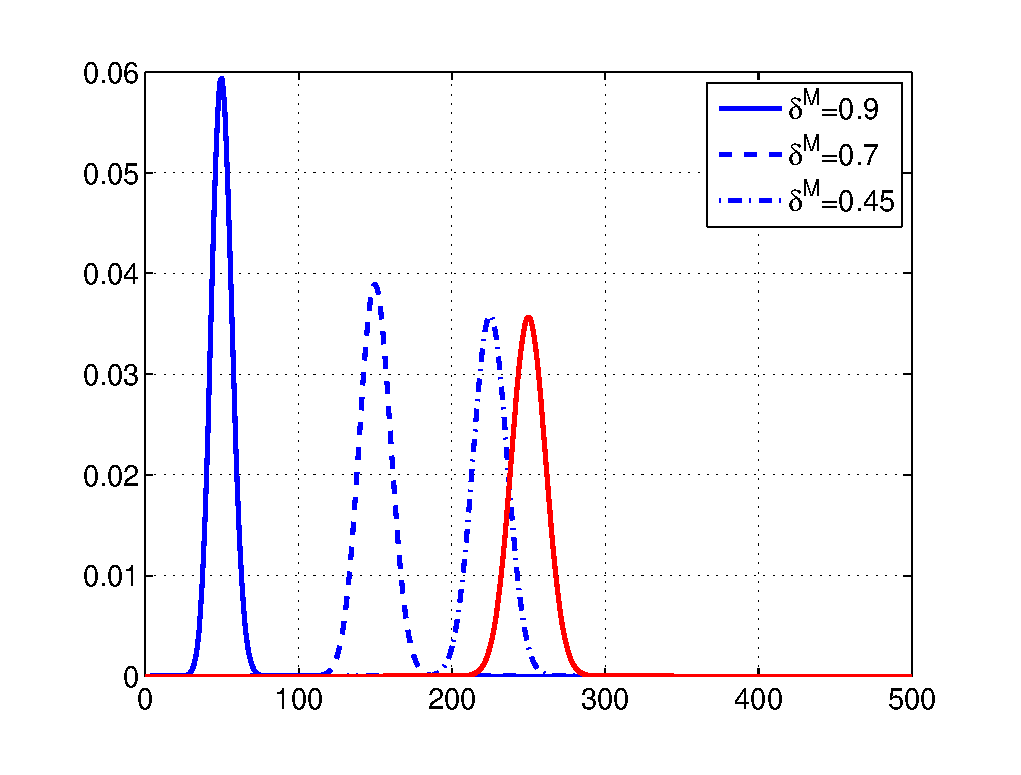
\includegraphics[width=0.5\textwidth]{deltaMexample2a}}
            {\includegraphics[width=0.5\textwidth]{deltaMexample2b}}}
\caption{\label{deltaMexample2}The left figure shows how one can evaluate the lower and upper
bounds of $|\omega^k-\bar{\omega}|_{TV}$, where $\omega^0$ has the form in equation (\ref{expw0}),
by finding the overlap area of two binomial distributions centered at
$p\delta_k=\frac{1}{2}+\epsilon r^k$ and $p/2$. In the right figure the upper bound and the lower
bound of $|\omega^k-\bar{\omega}|_{TV}$ by Theorems \ref{theoremub2} and \ref{theoremlb} are plotted,
as well as their approximations by Theorem \ref{theoremapproxlb}.}
\end{figure}
This is valid for each $k$. Similar to Example \ref{example:constantoega0}, we can plot the upper and lower bounds in a reduced space to see the movement of a binomial distribution. The left plot of Figure \ref{deltaMexample2} shows how the upper bound distribution moves toward the binomial distribution
centered at $p/2$ when $k$ increases, and then the TVs of upper bound and lower bound versus iteration plot is given
in the right plot of Figure \ref{deltaMexample2} for $\delta_0= 1$ and $r=0.998$.
Again, from the change of the overlap area of the left plot, it is not hard to understand how the concave shape is formed in the right plot.  

We need to stress here that to find the actual $|\omega^k-\bar{\omega}|_{TV}$ trajectory is impossible because one needs to evaluate (\ref{infiniteTV}) for each $\omega^k$. Even just to find an approximation of it using (\ref{finiteTV}), the computation cost is extremely large. This demonstrates the value of the upper and lower bound theorems. However, even so, we do not get much insight on how the bounds evolve because these two theorems give bounds based on the incomplete beta function. Hence here we would like to apply Theorem \ref{theoremapproxlb} regardless of its condition ($p \to \infty$ and $\delta_\star \to 1$). It should give us a pair of approximate upper and lower bounds,
\begin{eqnarray}
\label{expub}
|\omega^k -\bar{\omega}|_{TV}  &\stackrel{approx.}{\le}  &  \erf\left( \sqrt{\frac{p}{2}}\left((\delta_{\star}^M)^k-\frac{1}{2}\right)\right) \nonumber \\
                               & = &     \erf\left( \sqrt{\frac{1}{2(1-r)}} \epsilon^0r^k \right),
\end{eqnarray}
and
\begin{eqnarray}
\label{explb}
|\omega^k -\bar{\omega}|_{TV}  &\stackrel{approx.}{\ge} & \erf\left( \sqrt{\frac{1}{2(1-r)}} \epsilon^0 r^{\frac{1}{1-r}}r^k \right)  \nonumber \\
                               & = &  \erf\left( \sqrt{\frac{1}{2(1-r)}} \epsilon^0 e^{-1} r^k \right).
\end{eqnarray}
The approximated upper and lower bounds are plotted in the right of Figure \ref{deltaMexample2}, too. They are almost identical to the actual bounds.
Both (\ref{explb}) and (\ref{expub}) show the normal shapes, just like we see in example 1. Since
$(\delta_{\star}^M)^k-\frac{1}{2} = \epsilon^0 r^k$ decays exponentially (with factor $r$) to $0$, the trajectory
does not look like the error function itself. Instead, it has a sharper change before cutoff
happens and gets milder after it.
\end{example}
%%%%%%%%%%%%%%%%%%%%%%%%%%%%%%%%%%%%%%%%%%%%%%%%%%%%%%%%%%%%%%%%%%%%%%%%%%%%%%%%%%%%

The above two examples show the impact of $p$ and $\delta_{\star}^M$, which relate to the sum of
the stochastic symbol sequence and its largest entry. To summarize, the TV of the current distribution to the invariant distribution can be characterized by its upper and lower bounds, which correspond to $|\psi( (\delta^m)^k )^{-1}-\bar{\omega}|_{TV}$ and $|\psi( (\delta^M)^k )^{-1}-\bar{\omega}|_{TV}$. They
can be evaluated (and also approximated) and then the shape of $|\omega-\bar{\omega}|_{TV}$ is determined.
% which
%centered at $p\delta_{\star}^M$ (resp. $p\delta_{\star}^m$) and $p/2$. And so their TV can be bounded by $p$ and $\delta_{\star}^M$ (resp. $\delta_{\star}^m$). Isolating the
%change of $p$ or $\delta_{\star}^M$($\delta_{\star}^m$), the trajectory can be shown as the right
%plot of figure \ref{deltaMexample1} and the right plot of figure \ref{deltaMexample2}.



\subsection{Create cutoffs}
We have shown that an initial distribution like (\ref{expw0}) evolved by $P_S$ can have very similar $|\omega^k-\bar{\omega}|_{TV}$ trajectory to what one sees in a cutoff phenomenon. Now we want to take a further step to show that we can generate a set of initial disitributions $\omega_n$, which are a function of $n$, such that $\nu_n^k = |\omega_n^k-\bar{\omega}|_{TV}$ actually has the shape of (\ref{rdwalkshape}) when $n$ goes to infinity. We give the following theorem.
%%%%%%%%%%%%%%%%%%%%%%%%%%%%%%%%%%%%%%%%%%%%%%%%%%%%%%%%%%%%%%%%%%%%%%%%%%%%%%%%%%%%%
\begin{theorem}
Let $\omega_n^0 \in \bar{\Omega}$ have stochastic symbol sequence
 \begin{eqnarray}
    \psi(\omega^0_n) =  \{.\delta_0 \delta_1 \delta_2 \cdots\},
 \end{eqnarray}
where $\delta_i = \min\{\frac{1}{2}+\epsilon_n r_n^i,1\}$, and
 \begin{align}
 \begin{split}
          r_n &= e^{-\frac{2}{n}}.\\
          \epsilon_n &= \sqrt{\frac{n(1-r_n)}{4}},
 \end{split}
 \end{align}
The family $(\Omega,\bar{\omega},(\omega^k_n)_{k=0,1,\ldots})_{n=1,2,\ldots}$ presents a total variation-cutoff. In fact, 
Let $k = \frac{1}{4}n\log{n}+cn $; then for fixed $c\in \mathbb{R}$ as $n\to \infty$,
\begin{eqnarray}
\label{erfbound}
 %|\omega^k_n - \bar{\omega} |_{TV} \sim \erf \left(\frac{e^{-2c}}{\sqrt{8}}\right)
          \erf \left(\frac{e^{-2c-1}}{\sqrt{8}}\right)\le  |\omega^k_n - \bar{\omega} |_{TV} \le \erf \left(\frac{e^{-2c}}{\sqrt{8}}\right).
\end{eqnarray}
\end{theorem}

\begin{proof} From example 3, $|\omega^k_n - \bar{\omega}|_{TV}$ is bounded by (\ref{omegakbound}). When $n \to \infty$, $\epsilon_n$ goes to $\sqrt{\frac{1}{2}}$ and $r_n$ goes to $1$. Letting $k> \frac{-\log(2\epsilon_n)}{r_n}$ so that $\epsilon_n r_n^k<1/2$, and using the results of (\ref{expub}) and (\ref{explb}), we have
\begin{eqnarray}
                \erf\left( \sqrt{\frac{1}{2(1-r_n)}} \epsilon_n e^{-1} r_n^k \right)
            \le |\omega^k_n - \bar{\omega}|_{TV}
            \le \erf\left( \sqrt{\frac{1}{2(1-r_n)}} \epsilon_nr_n^k \right).
\end{eqnarray}
Now these bounds are not approximations because the conditions of Theorem \ref{theoremapproxlb} are satisfied. 
Substituting the expresstion $\epsilon_n$ and $r_n$ into above inequality gives
\begin{eqnarray}
                \erf\left(\sqrt{\frac{n}{8}}e^{-\frac{2k}{n}-1}  \right)
            \le |\omega^k_n - \bar{\omega}|_{TV}
            \le  \erf\left(\sqrt{\frac{n}{8}}e^{-\frac{2k}{n}}  \right),
\end{eqnarray}
%Thus we have
%\begin{eqnarray}
  %     |\omega^k_n - \bar{\omega} |_{TV} \sim \erf\left(\sqrt{\frac{n}{8}}e^{-\frac{2k}{n}}  \right)
%\end{eqnarray}
Letting $k = \frac{1}{4}n\log{n}+cn $ for $c\in \mathbb{R}$, and substituting into the above expression, we get the desired result (\ref{erfbound}), and hence it presents a cutoff.
\end{proof}

%%%%%%%%%%%%%%%%%%%%%%%%%%%%%%%%%%%%%%%%%%%%%%%%%%%%%%%%%%%%%%%%%%%%%%%%%%%%%%%%%%%%%%

The key idea of the above theorem is that we know for a pair of $(\epsilon,r)$, the stochastic symbol sequence with $\delta_i = \frac{1}{2}+\epsilon r^i$ has a normal shape cutoff. Hence we equate the coefficients to find $(\epsilon_n,r_n)$ as functions of $n$ that have the same $|\omega^k_n - \bar{\omega} |_{TV}$ as the random walk on a $n$-dimensional hypercube problem. In this case the $\epsilon_n$ we find is larger than $1/2$ when $n>1$, which is prohibited in the stochastic symbol sequence ($\delta_0>1$). However, we set $\delta^i=1$ for $i<\frac{-\log(2\epsilon_n)}{r_n}$ and then when $k> \frac{-\log(2\epsilon_n)}{r_n}$, the remaining sequence is exponential and Theorem \ref{theoremapproxlb} is applicable again.

Following the same rule, we can reproduce any cutoff with normal shape in relaxed sense by a family $\{\Omega,\bar{\omega},(\omega_n^k)_{k=0,1,\ldots}\}_{n=0,1,\ldots}$, where $\omega_n^{k+1} = P_S(\omega_n^k)$, and $P_S$ is the Perron-Frobenius of map $S:\Lambda \to \Lambda$, which has symbolic dynamics.


%%%%%%%%%%%%%%%%%%%%%%%%%%%%%%%%%%%%%%%%%%%%%%%%
\subsection{What causes cutoffs?}
%%%%%%%%%%%%%%%%%%%%%%%%%%%%%%%%%%%%%%%%%%%%%%%%
As we have mentioned before, the analysis and proof of cutoffs are usually very hard, but to understand what causes cutoffs can be quite easy and we discuss it here to further explain the relation between the cutoff of finite Markov Chains and chaotic map mixing. Let us focus on the total variation-cutoff with normal shape. We claim that if the process is composed of many (almost) independent small processes, then it has the key factor to present a cutoff. To explain this, again we use the random walk on an $n$-dimensional hypercube as the example. Let $I=\{0,1\}$; the coordinate of the particle can be represented as a vector in $I^n$. For instance, the point starting at the origin is
\begin{eqnarray*}
 x^0 = (0,0,\ldots,0).
\end{eqnarray*}
Each of the coordinates equals zero with probability $1$. At each iteration, the particle can stay fixed or choose one of the coordinates randomly. For this chosen coordinate, if it is $0$, it becomes $1$ and vice versa. Under this big process with $n$ coordinates and $2^n$ states, we can discuss $n$ much smaller random processes: the value of each coordinate. All of these small processes are not independent of each other. For example, at iteration $1$, suppose we know that the first coordinate is $1$; then we immediately know all of the other coordinates are zeros. 
So even though all of these small processes are identical and easy to analyze, to calculate the probability of the $2^n$ states by the joint probability of the small processes is still not possible. Nonetheless, a very important fact is: they become almost independent after just several iterations. This is also easy to imagine: suppose $n = 1000$ and $k = 10$; knowing that the first coordinate is $1$ is almost not helpful to know the value of any other coordinates. The tendency that these small processes have to become independent of each other is so strong that even if we just assume they are independent in the beginning, and calculate $\omega_n^k$ by the joint probability of these independent small processes, we get a very good approximation of the actual process. This simplification corresponds to the continuous-time random walk on a hypercube problem \cite{Diaconis1990}. The analysis of this problem is much easier than the original problem and it presents the same cutoff. Therefore, we can conclude that even if the original process is very complicated, the almost independence of the small processes is the key for the whole process to present a cutoff. 

Then how does this almost independence fit into the chaotic map evolution? Remember that the probability space we discuss is $\bar{\Omega}$, and from Lemma \ref{lemma:independency}, when a point $x$ with probability distribution $\omega \in \bar{\Omega}$ is evolved by the chaotic map with symbolic dynamics, $\phi(x^k)_i$ and $\phi(x^k)_j$ are independent of each other for all $k$ and $i\neq j$. So this process looks like it is composed of an infinite number of independent small processes. Thus we can design the exponential type stochastic symbol sequence to make all these small processes behave like the process we see in one coordinate of the hypercube and achieve similar TV trajectories. It is purely the special property of $\omega \in \bar{\Omega}$ for chaotic maps with symbolic dynamics that makes this possible. This clearly explains why we observe cutoffs in chaotic map evolution.  

 

%%%%%%%%%%%%%%%%%%%%%%%%%%%%%%%%%%%%%%%%%%%%%%%%
%\subsection{When $\omega \notin \bar{\Omega}$}
%%%%%%%%%%%%%%%%%%%%%%%%%%%%%%%%%%%%%%%%%%%%%%%%

%The above results are only applicable when $\omega \in \bar{\Omega}$, and is quite restrictive. An easy extension can be made for all $\omega \in \Omega$ and are ``close'' to $\bar{\Omega}$ in total variation distance. Given $\omega^0 \in \Omega $, suppose we can find an $\tilde{\omega}^0\in \bar{\Omega} $ such that $|\omega^0- \tilde{\omega}^0|_{TV}$ is small, then use triangular inequality, for any $k \ge 0$
%\begin{eqnarray}
%     \left| |\tilde{\omega}^k-\bar{\omega} |_{TV}  -  |\omega^k-\tilde{\omega}^k|_{TV}\right|
%     \le |\omega^k-\bar{\omega}|_{TV}
%     \le |\tilde{\omega}^k-\bar{\omega}|_{TV} + |\omega^k-\tilde{\omega}^k|_{TV}
%\end{eqnarray}
%Total variation distance is non-increasing, thus $|\omega^k-\tilde{\omega}^k|_{TV} \le |\omega^0-\tilde{\omega}^0|_{TV} $. Let the upper and lower bounds obtained by theorem \ref{theoremub} and \ref{theoremlb} for $|\tilde{\omega}^k-\bar{\omega} |_{TV}$ be $b_l^k$ and $b_u^k$, and let $|\omega^0-\tilde{\omega}^0|_{TV} = b^0$, we have
%\begin{eqnarray}
%     |b_l^k-b^0| \le |\omega^k-\bar{\omega}|_{TV}  \le b_u^k+b^0
%\end{eqnarray}
%How do we find $\tilde{\omega}^0$ such that $|\omega^0- \tilde{\omega}^0|_{TV}$ is minimized so that the bound is tighter? The easiest way is letting $\tilde{\omega}^0 = \psi(\omega^0) $. This may not be the best fitting of $\omega^0$, however, it is believed that if $\psi(\omega^0)$ is not a good fitting of $\omega^0$, there is not much space to improved by finding another $\tilde{\omega}^0$. Again, we want to stress that the upper and lower bounds are not practically useful, but they do characterize the behavior of the convergence trajectory for a set of $\omega^0$.



%
% Conclusion
%
\section{Conclusion}
\label{sec:symdynconclusion}
In this article we generalize symbolic dynamics for chaotic maps and define a new object called
stochastic symbol sequence. For a set of probability distributions in the reduced space
$\bar{\Omega}$, they can be evolved easily by a shift operator, and the total variation distance to
the invariant distribution can be bounded by the distance between two binomial distributions. We
show that for the distribution $\omega^0$ with stochastic symbol sequence $\delta_i=1/2+\epsilon
r^i$, $r \to 1$, its $|\omega^k-\bar{\omega}|_{TV}$ has normal shape. Thus we can generate
a sequence of $\omega^0_n$ to produce a sequence of cutoff trajectories that have the same
limiting behavior as the ones found in the random walk on an $n$-dimensional hypercube problem. This
result can be generalized to other cutoffs with normal shape in finite Markov Chains.

The above result not only demonstrates the close relationship between cutoff phenomenon studies in finite Markov Chain and chaotic maps, but also points out the source of cutoffs: almost independence of the underlying small processes. This can be very useful for the study of large systems. So far there are not many good tools to understand and analyze very large systems. However, if we can identify each of the small processes in the large system and justify their almost independence, cutoffs can be proved. 

The relation between chaos and cutoff phenomenon has also been found in numerical studies and
experiments. In \cite{numcutoff}, the author provides numerical evidence to show that the
variance of Standard Map presents a cutoff when the diffusion goes to zero. In \cite{topopt} a
numerical simulation of a chaotic mixing channel also shows cutoffs in mixing trajectories. More
numerical evidence can be found in \cite{Thiffeault2003-13, Tsang2005}, though they do not call
the phenomenon cutoff. The above studies focus on the convergence trajectories of the variance of a
scalar function advected by 2-D chaotic maps with small diffusion---a different content from the study here. However, just as it is believed that cutoff phenomenon is widespread in many
finite Markov Chains, we believe cutoffs are intrinsic for chaotic maps, not only for the
distribution inside or close to $\bar{\Omega}$.


%%
% Body
%
%%%%%%%%%%%%%%%%%%%%%%%%%%%%%%%%%%%%%%%%%%%%%%%%%%%%%%%%%%
%%%%%%%%%%%%%%%%%%%%%%%%%%%%%%%%%%%%%%%%%%%%%%%%%%%%%%%%%%
\section{Background}
\label{sec:background}
%%%%%%%%%%%%%%%%%%%%%%%%%%%%%%%%%%%%%%%%%%%%%%%%%%%%%%%%%%
%%%%%%%%%%%%%%%%%%%%%%%%%%%%%%%%%%%%%%%%%%%%%%%%%%%%%%%%%%

\paragraph{Cutoff phenomenon.} Cutoff phenomenon was discovered by Aldous, Diaconis, and Shahshahani \cite{Diaconis1987, Diaconis1986, Diaconis1981}, and
formalized by Aldous and Diaconis \cite{Diaconis1996, Diaconis1987}. The most interesting cases are found in the random walks on finite
groups with the measure of total variation distance, and most known Markov Chains that present cutoffs can be shown to belong to this
category \cite{LSaloff-Costt2004}. Here we state the definition of a cutoff given by Diaconis in \cite{Diaconis2005}. Assume that to any
finite set $\Omega$ and any pair of probability measures $\omega$, $\bar{\omega}$ on $\Omega$ is associated a real number
$D(\omega,\bar{\omega})$ such that $D(\omega,\bar{\omega})\in [0,1]$,
\begin{eqnarray}
\max_{\Omega,\omega,\bar{\omega}} D(\omega,\bar{\omega}) = 1,
\end{eqnarray}
and $D(\omega,\bar{\omega})=0$ if and only if $\bar{\omega}=\omega$. Consider a sequence of
(finite) probability spaces $(\Omega_n,\bar{\omega}_n)$, $n=1,2,\ldots\ $, each equipped with a sequence
of probability measure $\omega^k_n$, $k=0,1,\ldots\ $, such that
\begin{eqnarray}
\lim_{k \to \infty} D(\omega_n,\bar{\omega}_n)=0.
\end{eqnarray}
The definition of a cutoff follows,

\begin{definition}
\label{cutoffdefinitions} (Diaconis) A family $(\Omega_n,\bar{\omega}_n, (\omega^k_n)_{k=0,1,\ldots})_{n=1,2,\ldots}$ presents a D-cutoff if
there exists a sequence $(t_n)$ of positive reals such that, for any $\epsilon \in(0,1)$,
\begin{enumerate}
  \item $\lim_{n \to \infty}D(\omega^{k_n}_n,\bar{\omega}_n) = 0 \mbox{ if }
  k_n>(1+\epsilon)t_n;$
  \item $\lim_{n \to \infty}D(\omega^{k_n}_n,\bar{\omega}_n) = 1 \mbox{ if }
  k_n<(1-\epsilon)t_n.$
\end{enumerate}
\end{definition}

Cutoff phenomenon is defined for finite Markov Chains and in most cases the Markov transition matrices are generated by symmetric groups.
Since this does not fit our applications in chaotic mixing, we relax the definition and set $\Omega_n$ to be infinite. We say that
a family $(\Omega_n,\bar{\omega}_n, (\omega^k_n)_{k=0,1,\ldots})_{n=1,2,\ldots}$ presents a D-cutoff in the relaxed sense if it satisfies
Definition \ref{cutoffdefinitions} but $\Omega_n$ is infinite. 
%However once the definition is relaxed, the initial distribution is not obvious for each chains and need to be specified.

The distance function we use is the total variation distance.
\begin{definition} For two finite probability distributions $\mu$ and $\nu$, the \textbf{total variation
distance} (TV) between $\mu$ and $\nu$ is
  \begin{eqnarray*}
   |\mu - \nu|_{TV} = \frac{1}{2}\sum_{i} |\mu(i)-\nu(i) |.
  \end{eqnarray*}
\end{definition}
For continuous probability distributions, simply replace the summation by an integration.


The shape of a cutoff can be characterized in several ways \cite{Chen2006}. We are specifically interested in the
``normal'' shape, which is addressed by the following famous cutoff example.

\begin{example} \textbf{Random walk on an $n$-dimensional hypercube} (Diaconis \cite{Diaconis1990})
a particle starts at $\mathbf{0}$ and moves to one of its nearest neighbors (or stay fixed) with equal probability at each step. Let $k =
\frac{1}{4}n\log{n}+cn$. Then for fixed $c \in \mathbb{R}$, as $n \to \infty$,
\begin{eqnarray}
\label{rdwalkshape}
 |\omega^k_n - \bar{\omega} |_{TV} \sim \erf \left(\frac{e^{-2c}}{\sqrt{8}}\right).
\end{eqnarray}
In this example, the cutoff shape is called ``normal'' because of the close relation between normal distribution and error function. In fact, most interesting cutoff examples have normal shapes. When $n \to \infty$ their evolution of total variation distance to uniform can be calculated by evaluating the TV between two normal distributions. This fact becomes crucial in our later discussion. 

\todo{TC: the TV between two normal distributions with the same variance and similar 
means is error function of the difference of their means}





\begin{figure}
\centerline{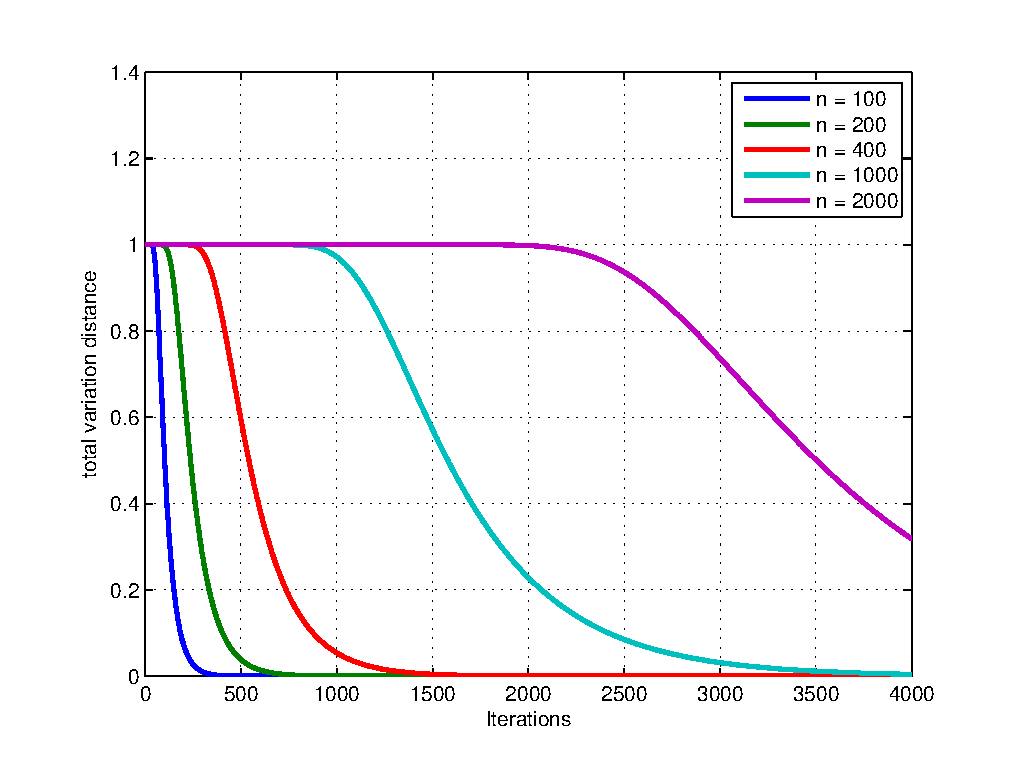
\includegraphics[width=0.7\textwidth,trim=1cm 1cm 0cm 0cm]{rdwalk}} \caption{The $k$
versus $|\omega_n^k-\bar{\omega}|_{TV}$ plot of random walk on an $n$-dimensional hypercube
problem. When $n$ increases, the distance stays close to $1$ for more iterations before it drops to
zero. }
\end{figure}

\end{example}

It is believed that cutoff phenomenon is widespread, although it has been proved only for a small
number of examples. The proof of cutoffs is in general very hard and varies case by case.


Although the study of cutoffs is focused on finite Markov Chains, we care more about what kind of
linear systems can generate convergence trajectories that have sharp changes. It is very hard
to image how a distribution would evolve abruptly to almost uniform from highly
concentrated (in a single state for finite Markov Chains). However, there is an excellent
explanation of why this happens. Consider another famous cutoff example: the Ehrenfest urn problem, involving $2$ urns and $n$
balls. In the beginning all the balls are in urn one, and at each iteration one of the balls is
chosen randomly and put in the other urn. This process is a Markov Chain and it can be shown that
this problem has the same total variation distance $|\omega^k_n-\bar{\omega}|_{TV}$ as the random
walk on hypercubes problem. In fact, this is how people analyze the random walk problem without
actually studying the $2^n$ system states. In this new Markov Chain, there are only $n+1$
states, which stand for the number of balls in urn $2$. In the beginning, all the balls are in urn
$1$ so the probability distribution is concentrated in the first state. The invariant distribution
of this reduced system is a binomial distribution centered at state $(n+1)/2$ (assuming $n$ is odd). By observing how the distribution is evolved when the system iterates, one would see two things:
first, the shape of the distribution gradually becomes binomial to fit the final shape; secondly,
the center of the distribution moves from $0$ toward $(n+1)/2$ at a certain speed (not a constant). When $n$ is large, not only does the center of the
distribution need more iterations to move to $(n+1)/2$, but also the shape of the distribution
needs more iterations to fit the stationary distribution. Cutoff is created by the combination of
these two effects. More details about this explanation can be found in \cite{Lloyd2005}. Now what decides the
shape of the cutoff when $n$ tends to infinity? When $n \to \infty$, a binomial distribution
can be well approximated by a normal distribution. Hence how the total variation distance changes near a
cutoff can be calculated by the TV of two normal distributions, and it has the
form like (\ref{rdwalkshape}). Therefore by forming the reduced system, we see clearly how a cutoff
can happen.





\paragraph{Chaotic Mixing.}
A widely observed phenomenon in the chaotic mixing process when small diffusion exists is the
two- or three-stage transition \cite{Thiffeault2003-13, Fereday2002, Antonsen1996}. The map
does not mix the scalar function with a constant rate in general. When the variance of the scalar
function is measured during the mixing process, one can in general observe a relatively flat decay
followed by a super-exponential change, and then finally it tends to an exponential decay. People
are interested in when these transitions happen, why they happen, and how to predict the slope of
the exponential region. A good review and physical interpretation can be found in
\cite{Thiffeault2004}.

In fact, such multi-stage mixing process can also be found in $1$-D chaotic map when a probability distribution is advected by the Perron-Frobenius operator of the map. To explain this, we first give the definition of the Perron-Frobenius operator \cite{Mezic2005}.

In the measure space $(X,\mathcal{A},\mu)$, for a map $S:X\to X$, we define the following operator. 
\begin{definition} \textbf{ (Perron-Frobenius operator)}
Let $\omega \in L^1(X)$, and suppose that for every $A \in \mathcal{A}$ the operator $P_S:L^1(X) \to L^1(X)$ satisfies
  \begin{eqnarray}
    \int_A P_S \omega(x)\mu(dx) = \int_{S^{-1}(A)} \omega(x)\mu(dx).
  \end{eqnarray}
Then $P_S$ is the Perron-Frobenius operator associated with $S$.
\end{definition}
It tells us how a probability distribution is evolved by a map $S$. 

%%%%%%%%%%%%%%%%%%%%%%%%%%%%%%%%%%%%%%%%%%%%%%
\begin{example} \textbf{Tent map cutoff.}
Consider the tent map
   \begin{eqnarray}
   \label{tentmap}
     x' = S_\text{tent}(x) = 1-2\left|x-\frac{1}{2}\right|
   \end{eqnarray}
with the following initial distributions on $[0 ,1]$:
  \begin{eqnarray}
  \label{tentmapinitial}
    \omega_n^0 = \begin{cases}
                      \frac{1}{\mu_n} &\text{ if } x \le \mu_n,\\
                      0               &\text{ otherwise},
                      \end{cases}
  \end{eqnarray}
where $\mu_1 = 1$, and $\mu_{n+1} = \mu_n/2$. The Perron-Frobenius operator of the tent map is
  \begin{eqnarray}
  \label{tentmapevolve}
    \omega_n^{k+1}(x) = P_\text{tent} \omega_n^{k}(x)
                             = \frac{1}{2}\left( \omega_n^{k}\left(\frac{x}{2}\right)+
                                                 \omega_n^{k}\left(1-\frac{x}{2}\right)  \right).
  \end{eqnarray}
The invariant distribution $\bar{\omega}$ of the tent map is uniform. Let $\nu_n^k =
|\omega_n^k-\bar{\omega} |_{TV}$; we find that
 \begin{eqnarray}
   \nu_n^k =  \begin{cases}
                    1- 2^{1+k-n}  &\text{ if }k \le n-1, \\
                    0             &\text{ otherwise}.
              \end{cases}
 \end{eqnarray}
The trajectories of $\nu_n^k$ with varying $n$ are shown in Figure \ref{tentmapcutoffplot}. It shows a cutoff.
\end{example}
%%%%%%%%%%%%%%%%%%%%%%%%%%%%%%%%%%%%%%%%%%%%%%%%
Hence we give the following simple theorem without proof.
%%%%%%%%%%%%%%%%%%%%%%%%%%%%%%%%%%%%%%%%%%%%%%%%
\begin{theorem} \textbf{(Tent map cutoff)}
\label{tentmapcutoff}
The family $(\Omega,\bar{\omega}, (\omega^k_n)_{k=0,1,\ldots})_{n=1,2,\ldots\,}$, where $\bar{\omega}$ is
uniform in $[0,1]$ and $\omega^k_n$ are defined as in (\ref{tentmapinitial}) and
(\ref{tentmapevolve}), presents a total variation-cutoff in the relaxed sense.
\end{theorem}
%%%%%%%%%%%%%%%%%%%%%%%%%%%%%%%%%%%%%%%%%%%%%%%%
A more general version of the above theorem and its proof can be found in section \ref{sec:mainresults}. Here we simply want to address that with the tent map and a sequence of suitable initial distributions, one can easily generate a sequence of Markov Chains that present a cutoff, though the shape is not normal.

This simple example shows that the tent map can present sharp changes in total variation distance. We would
like to generalize the result to a set of initial distributions and all $1$-D chaotic maps that have
full symbolic dynamics.



\begin{figure}
\centerline{{\includegraphics[width=0.7\textwidth]{tentmapcutoff.eps}}}
\caption{\label{tentmapcutoffplot} The plot of $\nu_n^k$. The trajectories present a cutoff.}
\end{figure}





%%%%%%%%
%%%%%%%%%%%%%%%%%%%%%%%%%%%%%%%%%%%%%%%%%%%%%%%%%%%%%%%%%%
%%%%%%%%%%%%%%%%%%%%%%%%%%%%%%%%%%%%%%%%%%%%%%%%%%%%%%%%%%
\section{Symbolic Dynamics and Stochastic Symbol Sequence}
\label{sec:symdyn}
%%%%%%%%%%%%%%%%%%%%%%%%%%%%%%%%%%%%%%%%%%%%%%%%%%%%%%%%%%
%%%%%%%%%%%%%%%%%%%%%%%%%%%%%%%%%%%%%%%%%%%%%%%%%%%%%%%%%%
%%%%%%%%%%%%%%%%%%%%%%%%%%%%%%
\subsection{Symbolic Dynamics}
%%%%%%%%%%%%%%%%%%%%%%%%%%%%%%
We briefly introduce symbolic dynamics for the study of chaotic maps. We focus on $1$-D chaotic maps, whose symbolic dynamics are semi-infinite sequences. 

Let $\mathcal{S}=\{L, R\}$ be the set of symbols consisting of $L$ and $R$. Define $\Sigma$, the collection of all semi-infinite sequence of elements of $\mathcal{S}$, i.e., $s\in \Sigma$ implies
 \begin{eqnarray}
 s= \{.s_0s_1\cdots s_n\cdots\}
 \end{eqnarray}
with $s_i\in \mathcal{S}$ for all $i$. We refer to $\Sigma$ as the space of semi-infinite sequence of two symbols. We consider a map $\sigma:\Sigma \to \Sigma$, which we shall call the shift map, defined as follows. For $s= \{.s_0s_1\cdots s_n\cdots\}$,
 \begin{eqnarray}
 \sigma(s)= \{.s_1s_2\cdots s_n\cdots\},
 \end{eqnarray}
i.e., the shift operator $\sigma$ simply deletes the first element of the sequence. There are rich results about the relation between symbolic dynamics and chaotic maps. Refer to \cite{Wiggins1990, Holmes1983} for good references. Roughly speaking, one can say that given a chaotic map $S$, on its invariant set $\Lambda$, the function $\phi(x): \Lambda \to \Sigma$, which maps a point in $x\in \Lambda$ to a semi-infinite sequence, is homeomorphism: $S$ acting on $\Lambda$ and $\sigma$ acting on $\Sigma$ are topologically conjugate. In other words, we have the following relation:
 \begin{eqnarray}
 S = \phi^{-1}\circ \sigma \circ \phi.
 \end{eqnarray}
And this explains the ``sensitive to initial condition'' property of chaotic maps.

All the results we derive in the next section in semi-infinite stochastic symbol sequences can be extended to bi-infinite ones without difficulty.

%Let $\mathcal{S}=\{L, R\}$ be the set of symbols consisting of $L$ and $R$. Let $\Sigma$ be the collection of all bi-infinite sequence of elements of $\mathcal{S}$, i.e., $s\in \Sigma$ implies
% \begin{eqnarray}
% s= \{\cdots s_{-n}\cdots s_{-1}.s_0s_1\cdots s_n\cdots\}
% \end{eqnarray}
%with $s_i\in \mathcal{S}$ for all $i$. We will refer to $\Sigma$ as the space of bi-infinite sequence of two symbols. We consider a map $\sigma:\Sigma \to \Sigma$, which we shall call the shift map, defined as follows: for $s= \{\cdots s_{-n}\cdots s_{-1}.s_0\cdots s_n\cdots\}$,
%  \begin{eqnarray}
% \sigma(s)= \{\cdots s_{-n}\cdots s_{-1}s_0.s_1\cdots s_n\cdots\}
% \end{eqnarray}
%$\sigma(\cdot)$ simply shift the dot one digit to the right of the sequence. There are rich results
%about the relation between symbolic dynamics and chaotic maps. Refer to \cite{Wiggins1990, Holmes1983} for good
%references. Roughly speaking, one can say that given a chaotic map $S$, on its invariant set
%$\Lambda$, the function $\phi(x): \Lambda \to \Sigma$, which maps a point in $x\in \Lambda$
%to a bi-infinite sequence, is homeomorphism: $S$ acting on $\Lambda$ and $\sigma$ acting on
%$\Sigma$ are topologically conjugate. In other words, we have the following relation,
% \begin{eqnarray}
% S = \phi^{-1}\circ \sigma \circ \phi
% \end{eqnarray}
%And this explains the ``sensitive to initial condition'' property of chaotic maps.

%In this paper we focus on the study of $1$-D chaotic maps, whose symbolic dynamics are semi-infinite sequences in stead of bi-infinite ones. 

%Define $\hat{\Sigma}$ the collection of all
%semi-infinite sequence of elements of $\mathcal{S}$. Each of the point $x \in \Lambda$ has $s\in
%\hat{\Sigma}$ with the following form,
% \begin{eqnarray}
% s= \{.s_0s_1\cdots s_n\cdots\}
% \end{eqnarray}
%The shift operator $\sigma$ simply deletes the first element of the sequence,
% \begin{eqnarray}
% \sigma(s)= \{.s_1s_2\cdots s_n\cdots\}
% \end{eqnarray}




%%%%%%%%%%%%%%%%%%%%%%%%%%%%%%%%%%%%%%%
\subsection{Stochastic Symbol Sequence}
%%%%%%%%%%%%%%%%%%%%%%%%%%%%%%%%%%%%%%%

Since our goal is to study how the probability density is evolved by the map, and symbolic dynamics
itself does not provide this information, we need a new object called stochastic symbol sequence.

%%%%%%%%%%%%%%%%%%%%%%%%%%%%%%%%%%%%%%%%%%%%%%%%%%%%%%%%%%%%%
% Definition
\begin{definition} \textbf{Stochastic symbol sequence.}
Consider $\mathcal{S}$ to be the symbol list. Let $\Delta$ be the collection of all
semi-infinite sequences of elements in $[0,1]$. We define $\delta^\star \in \Delta$ for each
symbol $\star \in \mathcal{S}$ as
 \begin{align}
 \begin{split}
 \delta^\star &= \{.\delta_0^\star \delta_1^\star\cdots \delta_n^\star\cdots\} \\
 %\delta^R &= \{\cdots \delta_{-n}^R\cdots \delta_{-1}^R.\delta_0^R \delta_1^R\cdots \delta_n^R\cdots\}
 \end{split} 
 \end{align}
with $\delta^\star_i \in [0,1]$ for all $i\ge 0$.
\end{definition}
%%%%%%%%%%%%%%%%%%%%%%%%%%%%%%%%%%%%%%%%%%%%%%%%%%%%%%%%%%%%%


The interpretation of each $\delta_i^\star$ is the probability of $x$ belonging to
symbol $\star$. Let $\Omega\in L^\infty[\Lambda], \int_\Lambda dz=1$ denote the space of
probability distribution in $\Lambda$. For a subspace  $\Lambda_\star \subset \Lambda$ and
$\omega\in \Omega$, we define $\psi^\star: \omega \mapsto \delta^\star$ as
 \begin{eqnarray}
 \label{psidef}
    %\delta^L_i = \int_{\Lambda_L} P^i_S \omega(z)dz \text{,   and  }
    \delta^\star_i = \int_{\Lambda_\star} P^i_S \omega(z)dz \text{, for all }i,
 \end{eqnarray}
where $P_S$ is the Perron-Frobenius operator of map $S$. Denote the $i$-th component of the symbolic dynamics of $x$ as $\phi(x)_i$. The above definition gives a simple relation between the symbolic dynamics and the stochastic symbol sequence. Suppose $x$ has pdf $\omega$, the stochastic symbol sequence of $\omega$ for symbol $\star \in \mathcal{S}$ is $\delta^\star$; then
 \begin{eqnarray}
 \label{deltaistar}
  \delta_i^\star = \prob(\phi(x)_i = \star) \text{, for } \star\in \mathcal{S} \text{ and all }i.
 \end{eqnarray} 

The definition is valid for any number of symbols. However, we only deal with two-symbol cases. For two-symbol cases: $\mathcal{S} = \{L,R\}$ and $\Lambda= \Lambda_L +\Lambda_R  $ , $\delta_i^R$ surely equals $1-\delta_i^L $. For simplicity, we
define $\psi = \psi^L$. We use $\delta$ to denote $\delta^L$ later. However, for clarity, we keep the $L$ for now. 


\begin{example} \textbf{Symbolic representation of the tent map}

Let $\Lambda=[0, 1]$. Partition $\Lambda \cap S^{-1}_{\text{tent}}(\Lambda)$ by writing its two
components as $\Lambda_L$ and $\Lambda_R$. For the tent map, $\Lambda_L=[0, 1/2]$ and $\Lambda_R=(1/2,1]$, we choose $\Lambda_R$ to exclude the point $1/2$ to avoid the overlap. We can associate with
each $x \in \Lambda $ a sequence $s = \{s_i \}_{i=0}^{\infty}$ of $L$'s and $R$'s defined by
$s_i=j$ if $S_{\text{tent}}^i(x) \in \Lambda_j$. The sequence ${s_i}$ labels the iterates of $x$
according to the left-right pattern they follow. In this way, we can label each $x \in \Lambda$
uniquely by a semi-infinite sequence $\phi(x)=s$ where the $s_i$'s are $L$'s and $R$'s. Let
$\Sigma$ denote the space of semi-infinite sequences of two symbols $L$'s and $R$'s. Then
$\phi(x): \Lambda \to \Sigma$ maps a point in $x\in I$ to a semi-infinite sequence.
The shift operator $\sigma$ acts on $s$ by simply dropping the first entry of $s$, i.e.,
$\sigma(\{s_i\}_{i=0}^{\infty})=\{s_i\}_{i=1}^{\infty}$. Similarly the map $\psi: \bar{\Omega}
\to \Delta$, where $\Delta$ denotes the space of semi-infinite stochastic
symbol sequence, maps an $\omega \in \bar{\Omega}$ to semi-infinite stochastic symbol sequences $\{
\delta^L,\delta^R\}$

%Note this is different from how it acts on a bi-infinity sequence, and this demonstrates that the
%tent map ``forgets'' the past information.
%An alternative interpretation of the semi-infinite
%sequence is as follows: one can embed the 1-D map into a 2-D volume preserved map, and make the
%symbol sequence bi-infinite. However, all the $s_i$'s with $i<0$ are unobservable. We can only
%evaluate (and we only care about) the thing happened in the first dimension.
\end{example}

It is clear that the map $\psi: \Omega \to \Delta $, as defined in
(\ref{psidef}), maps a probability distribution $\omega \in \Omega$ to the stochastic symbol
sequence $\delta$ uniquely. Moreover,  we overload the operator $\sigma$ to work
on the space $\Delta$, and have the following lemma.

%%%%%%%%%%%%%%%%%%%%%%%%%%%%%%%%%%%%%%%%%%%%%%%%%%%%%%%%%%%%%
%lemma
\begin{lemma}
  \begin{eqnarray}
 \psi \circ P_S = \sigma \circ \psi.
  \end{eqnarray}
\end{lemma}
\begin{proof} By definition,
  \begin{align}
      \delta_{i+1}^L (\omega)   &= \int_{\Lambda_L} P_S^{i+1} \omega(z)dz \nonumber\\
                                &= \int_{\Lambda_L} P_S^{i} \left(P_S\omega(z) \right) dz \nonumber\\
                                &=  \delta_{i}^L (P_S \omega).
  \end{align}
\end{proof}
%%%%%%%%%%%%%%%%%%%%%%%%%%%%%%%%%%%%%%%%%%%%%%%%%%%%%%%%%%%%%

However, unlike $\phi$, the function $\psi$ is not invertible. There are many $\omega$'s that map to the same $\delta^L$. To resolve this problem, for a given chaotic map $S$ we consider a smaller space:
  \begin{eqnarray}
  \label{DefOmegabar}
  \bar{\Omega} = \left\{ \omega \mid \omega(z) = \lim_{n \to \infty} \prod_{i=0}^n \beta^{\phi(z)_i}_i \right\},
  \end{eqnarray}
where $\beta^L_i \in [0,1]$, $\beta^R_i=1-\beta^L_i$. Remember that $\phi(z)_i$ is the $i$-th component of the symbol sequence of $z$ associated with the chaotic map, so having symbolic dynamics is a necessary condition for having $\bar{\Omega}$.

%%%%%%%%%%%%%%%%%%%%%%%%%%%%%%%%%%%%%%%%%%%%%%%%%%%%%%%%%%%%%
The following lemma justifies the existence of $\psi^{-1}$ in $\bar{\Omega}$.
%lemma
\begin{lemma} For $\omega \in \bar{\Omega}$, one has
 \begin{eqnarray}
    \delta^L_k(\omega) = \beta^L_k(\omega)  \text{, for all }k.
 \end{eqnarray}
\end{lemma}
\begin{proof} By definition,
 \begin{align}
    \delta_{k}^L (\omega)   &= \int_{\Lambda_L} P_S^{k} \omega(z)dz \nonumber\\
                            &= \int_{S^{-k}(\Lambda_L)} \omega(z)dz \nonumber\\
                            &= \lim_{n \to \infty} \sum_{\substack{s\in \Sigma\\s^k= L }}  \prod_{i=0}^{n} \beta^{s_i}_i \nonumber\\
                            &= \beta_k^L \lim_{n \to \infty} \sum_{s\in \Sigma}  \prod_{\substack{i=0\\ i\neq k}}^{n} \beta^{s_i}_i \nonumber\\
                            &= \beta_k^L.
 \end{align}
\end{proof}
%%%%%%%%%%%%%%%%%%%%%%%%%%%%%%%%%%%%%%%%%%%%%%%%%%%%%%%%%%%%%

Hence, in $\bar{\Omega}$ the map $\psi$ is invertible. From now on, the probability space we are interested in is the space $\bar{\Omega}$. It is also easy to check that
 \begin{eqnarray}
 \label{Pconserve}
  P_S (\omega) \in \bar{\Omega}, \mbox{ if } \omega \in \bar{\Omega}.
 \end{eqnarray}
And since $\psi$ is invertible, just like in symbolic dynamics, we also have
 \begin{eqnarray}
 P_S= \psi^{-1}\circ \sigma \circ \psi.
 \end{eqnarray}
It says the Perron-Frobenius operator and the shift operator are conjugate in the spaces $\{\bar{\Omega},\Delta \}$. To understand the special property of the subspace $\bar{\Omega}$, we give the following lemma.

%%%%%%%%%%%%%%%%%%%%%%%%%%%%%%%%%%%%%%%%%%%%%%%%%%%%%%%%%%%%%
%lemma
\begin{lemma} \label{lemma:independency}
For $x \in \Lambda$ having pdf $\omega \in \bar{\Omega}$, and any $s\in \Sigma$, then for any $i,j$, $i\neq j$, 
\begin{equation}
   \phi(x)_i=s_i \mbox{ and } \phi(x)_j=s_j \mbox{ are independent.}
\end{equation}
\end{lemma}
\todo{TC: there might be a better way to state the independence, and need to check is the proof strong enough.}
%one has
% \begin{equation}
%    \prob(\phi(x)_i=s_i) =   \prob(\phi(x)_i=s_i \mid  \phi(x)_k=s_k, k= {0,\ldots,\infty\}, k \neq i )
% \end{equation}
%\end{lemma}

\begin{proof} For $\omega\in \bar{\Omega}$, 
 \begin{align*}
   \prob(\phi(x)=s) &= \lim_{n \to \infty} \prod_{i=0}^{n} \delta_i^{s_i}  \\
                      &=  \lim_{n \to \infty} \prod_{i=0}^{n} \prob(\phi(x)_i=s_i).
 \end{align*}
The second equality is from equation (\ref{deltaistar}). This justifies the claim of independence.   
\end{proof}
%%%%%%%%%%%%%%%%%%%%%%%%%%%%%%%%%%%%%%%%%%%%%%%%%%%%%%%%%%%%%


Furthermore, we define the convex combination of two stochastic symbol sequences to be the convex combination of the individual components and then give another important property of the function $\psi$.
%%%%%%%%%%%%%%%%%%%%%%%%%%%%%%%%%%%%%%%%%%%%%%%%%%%%%%%%%%%%%
%lemma
\begin{lemma}
For any $\omega_1, \omega_2 \in \bar{\Omega}$ and $\alpha\in[0,1]$, one has
 \begin{eqnarray}
 \label{psiislinear}
  \psi(\alpha\omega_1+(1-\alpha)\omega_2) = \alpha\psi(\omega_1)+(1-\alpha)\psi(\omega_2).
 \end{eqnarray}
\end{lemma}

\begin{proof}
  \begin{align}
    \lefteqn{\alpha \delta^L_k(\omega_1) + (1-\alpha) \delta^L_k(\omega_2) } \nonumber\\
                    &=   \alpha \int_{S^{-k}(\Lambda_L)} \omega_1(z)dz+
                          (1-\alpha) \int_{S^{-k}(\Lambda_L)} \omega_2(z)dz \nonumber \\
                    &=   \int_{S^{-k}(\Lambda_L)}\left( \alpha \omega_1(z) +(1-\alpha) \omega_2(z) \right) dz \nonumber \\
                    &=   \delta^L_k( \alpha \omega_1 +(1-\alpha) \omega_2).
  \end{align}
\end{proof}
%%%%%%%%%%%%%%%%%%%%%%%%%%%%%%%%%%%%%%%%%%%%%%%%%%%%%%%%%%%%%
 This property can be extended to the convex combination of $n$ distributions and allows us to prove some important facts later.


We have successfully moved from the probability distribution $\omega \in \bar{\Omega}$ to its
stochastic symbol sequence representation. Now we would like to know how total variation distance
passes through, i.e., given $\omega$ and $\bar{\omega}$ with stochastic symbol sequence
$\{\delta^L, \delta^R\}$ and $\{\bar{\delta}^L,\bar{\delta}^R \}$, respectively, how do we calculate
$|\omega-\bar{\omega}|_{TV}$? The answer is:
 \begin{eqnarray}
 \label{infiniteTV}
|\omega-\bar{\omega}|_{TV} = \frac{1}{2} \lim_{n \to \infty}  \sum_{s\in\Sigma} \left| \prod_{i=0}^n\delta_i^{s_i}-\prod_{i=0}^n\bar{\delta}_i^{s_i}  \right|.
 \end{eqnarray}
This expression is almost impossible to evaluate because of the summation over infinity combinations. So let us consider a simpler case, when $\delta^L$ and $\bar{\delta}^L$ only have $p$ different digits, i.e.,\ $\delta_i^L = \bar{\delta}_i^L$ when $i\notin \theta$, and $|\theta| = p$. Let $\Sigma_p$ be the space of all combinations of $p$ symbol sequence with two symbols. Then we have
 \begin{eqnarray}
  \label{finiteTV}
|\omega-\bar{\omega}|_{TV} = \frac{1}{2} \sum_{s\in\Sigma_p}  \left| \prod_{i\in \theta}\delta_i^{s_i}-\prod_{i\in\theta}\bar{\delta}_i^{s_i}  \right|.
 \end{eqnarray}
In this expression, $s$ is some finite selections of the bi-infinite symbol sequence. The message here is that the total variation distance has nothing to do with the order: it only depends on the elements $s_i, i\in\theta$. Furthermore, (\ref{finiteTV})  can serve as a lower bound when the information besides $i\in \theta$ is unknown.







%%%%%%%%%%%%%%%%%%%%%%%%%%%%%%%%%%%%%%%%%%%%%%%%%%%%%%%%%%
\subsection{General results}
In reality, we may not care about the TV between two probability distributions, but want to know which one of them is closer to the invariant measure of the map. In this section, we give some general results about the TV from a stochastic symbol sequence of two symbols to the distribution $\bar{\omega}$, which has the representation
\begin{equation}
\label{deltabar}
\bar{\delta}=\left\{.\frac{1}{2}\frac{1}{2}\frac{1}{2}\cdots\right\}.
\end{equation}
Clearly (\ref{deltabar}) is invariant under the shift operator, and hence it is an invariant measure of the map. From now on we use $\delta$ to denote $\delta^L$, and if needed, $1-\delta$ represents $\delta^R$. Also, $\delta$ itself without any sub-index represents the whole stochastic symbol sequence, and $\delta_i$ indicates the $i$-th component in $\delta$ on the right-hand side of the dot.

\todo{TC:(\ref{deltabar}) is not the only invariant measure. Any constant sequence is invariant under the shift map, but we are not interested in them.}

The following convexity lemma is the basis of all later results.
%%%%%%%%%%%%%%%%%%%%%%%%%%%%%%%%%%%%%%%%%%%%%%%%%%%%%%%%%%%%%
%lemma
\begin{lemma} For $\delta,\delta^* \in \Delta$, $\alpha\in [0 ,1]$,
 \begin{eqnarray}
\label{convexityofTV}
|\psi^{-1}(\alpha\delta+(1-\alpha)\delta^*)-\bar{\omega}|_{TV} \le
            \alpha|\psi^{-1}(\delta)-\bar{\omega} |_{TV}+(1-\alpha)|\psi^{-1}(\delta^*)-\bar{\omega}|_{TV}.
 \end{eqnarray}
\end{lemma}
\begin{proof}
Since $\omega \mapsto |\omega-\bar{\omega}|_{TV}$ is a convex function, by using
(\ref{psiislinear}) we obtain that the function $\delta \mapsto
|\psi^{-1}(\delta)-\bar{\omega}|_{TV} $ is also convex. The convexity gives us the above
result.
\end{proof}
%%%%%%%%%%%%%%%%%%%%%%%%%%%%%%%%%%%%%%%%%%%%%%%%%%%%%%%%%%%%%



So even if there is no direct way to calculate the TV from a stochastic symbol
sequence to another, we can still use the convexity to deduce some useful bounds.

We give the following lemmas.

%%%%%%%%%%%%%%%%%%%%%%%%%%%%%%%%%%%%%%%%%%%%%%%%%%%%%%%%%%%%%
%lemma
\begin{lemma}
\label{onedifflemma} Suppose $\delta$ and $\delta^*$ are two stochastic symbol sequences corresponding
to the probability distribution $\omega$ and $\omega^*$, respectively. Suppose there exists a
bijection $\gamma: i \mapsto j$ such that $\delta_i = \delta^*_j$ for all $i\in
\mathbb{Z}\setminus\{i^\dagger\}$. If $ |\delta_{i^\dagger}-\frac{1}{2}| \ge |\delta^*_{\gamma(i^\dagger)}-\frac{1}{2}|$, then
 \begin{eqnarray}
      |\omega-\bar{\omega} |_{TV} \ge |\omega^*-\bar{\omega} |_{TV}.
 \end{eqnarray}
\end{lemma}
\begin{proof} Since $|\psi^{-1}(\delta)-\bar{\omega}|_{TV}$ is independent of the order of the sequence, we can assume
$\delta = \delta^*$ for all $i\in \mathbb{Z}\setminus\{i^\dagger\}$. Let $\tilde{\delta} = \delta$
for all $i\in \mathbb{Z}\setminus\{i^\dagger\}$, and
$\tilde{\delta}_{i^\dagger}=1-\delta_{i^\dagger}$. Apparently,
$|\psi^{-1}(\delta)-\bar{\omega}|_{TV} =|\psi^{-1}(\tilde{\delta})-\bar{\omega}|_{TV} $. When
$|\delta_{i^\dagger}-\frac{1}{2}| \ge |\delta^*_{i^\dagger}-\frac{1}{2}|$, it is always possible to
choose $\alpha\in[0,1]$ such that  $\delta^*_i = \alpha \delta_i +(1-\alpha) \tilde{\delta}_i $.
Applying (\ref{convexityofTV}) to $\delta$ and $\tilde{\delta}$ with the $\alpha$ above, we have
\begin{align}
    |\psi^{-1}(\delta^*)-\bar{\omega}|_{TV}
                 &\le  \alpha|\psi^{-1}(\delta)-\bar{\omega} |_{TV}+(1-\alpha)|\psi^{-1}(\tilde{\delta})-\bar{\omega}|_{TV} \nonumber\\
                 & =  |\psi^{-1}(\delta)-\bar{\omega} |_{TV}.
 \end{align}
\end{proof}
%%%%%%%%%%%%%%%%%%%%%%%%%%%%%%%%%%%%%%%%%%%%%%%%%%%%%%%%%%%%%

%%%%%%%%%%%%%%%%%%%%%%%%%%%%%%%%%%%%%%%%%%%%%%%%%%%%%%%%%%%%%
%lemma
\begin{lemma}
\label{alldifflemma} Suppose $\delta$ and $\delta^*$ are two stochastic symbol sequences corresponding
to the probability distribution $\omega$ and $\omega^*$, respectively. Suppose there exists a
bijection $\gamma: i \mapsto j$ such that $|\delta_i-\frac{1}{2}| \ge |\delta^*_j-\frac{1}{2} |$ for
all $i\in \mathbb{Z}$. Then
 \begin{eqnarray}
   |\omega-\bar{\omega} |_{TV} \ge|\omega^*-\bar{\omega} |_{TV}.
 \end{eqnarray}
\end{lemma}
\begin{proof} Apply Lemma \ref{onedifflemma} repeatedly.
\end{proof}
%%%%%%%%%%%%%%%%%%%%%%%%%%%%%%%%%%%%%%%%%%%%%%%%%%%%%%%%%%%%%

The above lemma tells us how to compare $|\omega-\bar{\omega}|_{TV}$ and $|\omega^*-\bar{\omega}|_{TV}$
if some relation of their stochastic symbol sequences is known. Now for a given $\omega$ we want
to bound its $|\omega-\bar{\omega}|_{TV}$ by choosing an $\omega^*$ such that its
$|\omega^*-\bar{\omega}|_{TV}$ is easy to calculate. The choices we made are the sequences with the
following form:
  \begin{align}
  \begin{split}
  \label{deltamM}
   \delta^m &= \{.\underbrace{\delta^m_{\star} \delta^m_{\star} \cdots \delta^m_{\star}}_{p}\frac{1}{2}\frac{1}{2}\cdots \}, \\
   \delta^M &= \{.\underbrace{\delta^M_{\star} \delta^M_{\star} \cdots \delta^M_{\star}}_{p}\frac{1}{2}\frac{1}{2}\cdots \}.
  \end{split}
  \end{align}
As we see later, $|\omega-\bar{\omega}|_{TV}$ can be evaluated easily if $\psi^{-1}(\omega)$ has finite constant leading terms. Note that we use the index $\star$ to indicate that $\delta_{\star}^M$ and $\delta_{\star}^m$ are numbers, not sequences.

  
%Where $\delta^m_0=\delta^m_1= \cdots = \delta^m_{p-1} \equiv \delta^m_{\star}$ and
%$\delta^M_0=\delta^M_1= \cdots = \delta^M_{p-1}\equiv \delta^M_{\star}$.


%First we are going to generalize the lower bound result from $\delta_i=1$, for $i\in \theta$ to $\delta_i=\delta^M$. Note here $\delta^M$ is a number, $1/2 \le \delta^M \le 1$.

%%%%%%%%%%%%%%%%%%%%%%%%%%%%
\subsubsection{Lower Bound}
%%%%%%%%%%%%%%%%%%%%%%%%%%%%%

%%%%%%%%%%%%%%%%%%%%%%%%%%%%%%%%%%%%%%%%%%%%%%%%%%%%%%%%%%%%%
%theorem
\begin{theorem}
\label{theoremlb} Suppose $\delta$ and $\bar{\delta}$ are two stochastic symbol sequences corresponding
to the probability distribution $\omega$ and the invariant distribution $\bar{\omega}$,
respectively. Suppose there is a set $\theta \subset \mathbb{Z}^++\{0\} $, $|\theta|=p$ such that
for all $i \in \theta$, $|\delta_i-\frac{1}{2}|>|\delta^m_\star-\frac{1}{2}|$. Then
\begin{eqnarray}
\label{lbineq}
|\omega-\bar{\omega}|_{TV} \ge \mathbf{I}_{\frac{1}{2}}(p-q^*,q^*+1) - \mathbf{I}_{1-\delta^m_\star}(p-q^*,q^*+1),
\end{eqnarray}
where
\begin{eqnarray}
\label{kstar}
q^* =  \left\lfloor p \frac{\log{2}+\log{(\frac{1}{2}-\epsilon)} }{\log{(\frac{1}{2}-\epsilon)}-\log{(\frac{1}{2}+\epsilon})} \right\rfloor,
\end{eqnarray}
$\epsilon = |\delta^m_\star-\frac{1}{2}|$, and $\mathbf{I}$ is the regularized incomplete
beta function.
\end{theorem}
\begin{proof}
Since the TV is independent of the order of the sequence, we can assume that
$\theta=\{0,1,\ldots,p-1\}$. Also, without loss of generality, we assume for $i\in \theta$,
$\delta_i \ge \epsilon+\frac{1}{2}= \delta^m_\star$. Using equation (\ref{finiteTV}) and Lemma
\ref{alldifflemma}, we have
\begin{align}
\label{lbtv}
|\omega-\bar{\omega}|_{TV}
                      &\ge \frac{1}{2} \sum_{s\in\Sigma_p}
                             \left| \prod_{i\in \theta}\delta_i^{s_i}-\prod_{i\in\theta}\bar{\delta}_i^{s_i}  \right| \nonumber\\
                      &\ge \frac{1}{2}  \sum_{q=0}^{p}
                             {p \choose q} \left|(\delta^m_\star)^q (1-\delta^m_\star)^{p-q} - \frac{1}{2^p} \right| \nonumber \\
                      &=   \frac{1}{2}  \sum_{q=0}^{p} \left|{p \choose q} (\delta^m_\star)^q (1-\delta^m_\star)^{p-q} -{p \choose q} \frac{1}{2^p} \right|.
\end{align}
\end{proof}
\todo{TC: The first line is an inequality because $p < \infty$. }

%%%%%%%%%%%%%%%%%%%%%%%%%%%%%%%%%%%%%%%%%%%%%%%%%%%%%%%%%%%%%

So the total variation distance can be lower bounded by the difference between two binomial
distributions. We can find their difference by subtracting their cumulative distribution functions
at the point they cross over each other. To do this we needs to find the point where the first
distribution begins to exceed the second distribution, which is to find the largest $q^*$ such that
\begin{eqnarray}
\left(\frac{1}{2}+\epsilon\right)^{q^*}\left(\frac{1}{2}-\epsilon\right)^{p-1-q^*}-2^{-p} \le 0.
\end{eqnarray}
Solving for $q^*$ gives (\ref{kstar}), and the cdf of a binomial distribution can be expressed in terms
of the regularized incomplete beta function $\mathbf{I}$ as follows. For the distribution
$\text{binomial}(r,p)$, its cdf is
\begin{eqnarray}
   F(q;p,r) = \mathbf{I}_{1-r}(p-q,q+1).
\end{eqnarray}
Substituting $q^*$ into $q$, and $1/2$ and $\delta^m_\star$ into $r$, we get (\ref{lbineq}).
%\begin{eqnarray}
%|\omega-\bar{\omega}|_{TV} \ge \mathbf{I}_{\frac{1}{2}}(p-k^*,k^*+1) - \mathbf{I}_{1-\delta^m}(p-k^*,k^*+1)
%\end{eqnarray}


An interesting corollary is that when $p$ goes to $\infty$, $|\omega-\bar{\omega}|_{TV}$ goes
to $1$ for all $\epsilon>0$. So each of the constant stochastic symbol sequences actually
represents an eigenfunction or an invariant measure of the map with eigenvalue $1$.




%%%%%%%%%%%%%%%%%%%%%%%%%%%
\subsubsection{Upper Bound}
%%%%%%%%%%%%%%%%%%%%%%%%%%%

We have seen that for a constant sequence with components not equal to $1/2$, the total variation
distance to the invariant distribution $\bar{\omega}$ is $1$ from the previous theorem. Hence this
result does not give us any information about the upper bound. We would like to bound the distance
by the sum of the sequence, and give the following theorem.
\begin{theorem}
\label{theoremub}Suppose $\delta$ and $\bar{\delta}$ are two stochastic symbol sequences corresponding
to the probability distribution $\omega$ and the invariant distribution $\bar{\omega}$,
respectively. Suppose $\sum_{i=0}^\infty |\delta_i - \frac{1}{2}| = \frac{M}{2}$. Then
\begin{eqnarray}
|\omega-\bar{\omega}|_{TV} \le  \begin{cases}
                                   \rho - 2^{-\lceil M \rceil } &\text{ if } \rho>1-2^{-\lceil M \rceil },\\
                                    1-2^{-\lfloor M \rfloor}    &\text{ otherwise},                                   \\
                                \end{cases} 
\end{eqnarray}
where $\rho = \frac{1}{2} +  \frac{M-\lfloor M \rfloor}{2}$.
\end{theorem}
\begin{proof}
With the convexity inequality (\ref{convexityofTV}), one can show that for a set of stochastic symbol sequence $\delta^j$, $j=\{1,2,\ldots\}$, $\sum_j{\alpha_j} = 1$,
\begin{eqnarray}
 \sum_j \alpha_j|\psi^{-1}(\delta^j)-\bar{\omega}|_{TV} \ge |\psi^{-1}(\sum_j \alpha_j \delta^j)-\bar{\omega}|_{TV}.
\end{eqnarray}
So for each $M$, if we can express $\delta$ as the convex combination of a set of $\delta^j$, the total variation distance $|\omega-\bar{\omega}|_{TV}$ can be bounded by the TV of individual $\delta^j$. Let the set $\mathbf{C} = \{\delta \, | \,\sum_i|\delta_i-\frac{1}{2}|  =  \frac{M}{2}\}$. It is easy to see that $\mathbf{C} = \mathbf{conv} \mathbf{D}$, where $\mathbf{D}$ is defined as
\begin{eqnarray}
  \mathbf{D}=\{\delta \mid \delta \text{ has } \lfloor M \rfloor \text{ } 1\text{'s, one } M-\lfloor M \rfloor
               \text{, and all other }\delta_i\text{'s are }\frac{1}{2}  \},
\end{eqnarray}
and $|\psi^{-1}(\delta)-\bar{\omega}(x)|_{TV}$ for each $\delta \in  \mathbf{D}$ can be calculated as
\begin{eqnarray}
|\psi^{-1}(\delta)-\bar{\omega}(x)|_{TV} = 
          \begin{cases}
             \rho - 2^{-\lceil M \rceil } &\text{ if } \rho>1-2^{-\lceil M \rceil },\\
             1-2^{-\lfloor M \rfloor}    &\text{ otherwise},                                   
          \end{cases}
\end{eqnarray}
where $\rho = \frac{1}{2} +  \frac{M-\lfloor M \rfloor}{2}$. We obtain the upper bound by choosing the set of $\delta^j$ to be $\mathbf{D}$.
\end{proof}

Unfortunately, the above upper bound is in general not very tight. We state it just to inspire the next theorem, which gives a tighter bound.
%%%%%%%%%%%%%%%%%%%%%%%%%%%%%%%%%%%%%%%%%%%%%%%%%%%%%%%%%%%%%%%%%%%%%%%%%%%%%%%%%%%%%%%%

\begin{theorem}
\label{theoremub2}
Suppose $\delta$ and $\bar{\delta}$ are two stochastic symbol sequences corresponding to the probability distribution $\omega$ and the invariant distribution $\bar{\omega}$, respectively. Suppose $\sum_{i=0}^\infty |\delta_i - \frac{1}{2}| = \frac{M}{2}$, and $\delta_i \le \delta^M_\star$ for all $i$. Then
\begin{eqnarray}
\label{ubineq}
|\omega-\bar{\omega}|_{TV} \le  \mathbf{I}_{\frac{1}{2}}(p-q^*,q^*+1) - \mathbf{I}_{1-\delta^M_\star}(p-q^*,q^*+1)
\end{eqnarray}
with
\begin{eqnarray}
\label{kstarub}
q^* =  \left\lfloor p \frac{\log{2}+\log{(\frac{1}{2}-\epsilon)} }{\log{(\frac{1}{2}-\epsilon)}-\log{(\frac{1}{2}+\epsilon})}  \right\rfloor,
\end{eqnarray}
where $\epsilon = |\delta^M_\star - \frac{1}{2}|$ and $p = \lceil \frac{M}{2\epsilon}\ \rceil$.
\end{theorem}

\begin{proof} Similarly to the previous proof, let
\begin{eqnarray}
  \mathbf{D}=\{\delta \mid \delta \text{ has } (p-1)\text{ }  of \text{ } \delta^M_\star\text{'s, one } M-(p-1) \delta^M_\star
                \text{, and all other }\delta_i\text{'s are }\frac{1}{2}   \}.
\end{eqnarray}
Then the set  $\mathbf{C} = \{\delta \mid \sum_i|\delta_i-\frac{1}{2}|  =  \frac{M}{2}\}$ satisfies $\mathbf{C} = \mathbf{conv} \mathbf{D}$. All $\delta \in \mathbf{D}$ have the same $|\psi^{-1}(\delta) - \bar{\omega}|_{TV} $ and are bounded by
\begin{eqnarray}
\label{middleineq}
 |\psi^{-1}(\delta) - \bar{\omega}|_{TV} < |\psi^{-1}(\delta^M) - \bar{\omega}|_{TV},
\end{eqnarray}
and $|\psi^{-1}(\delta^M) - \bar{\omega}|_{TV}$ can be calculated similarly to the lower bound proof by finding the $q^*$ such that the first binomial distribution is less than the second one, i.e., find the smallest $q^*$ such that
\begin{eqnarray}
\left(\frac{1}{2}+\epsilon\right)^{q^*}\left(\frac{1}{2}-\epsilon\right)^{p-q^*}-2^{-p} \ge 0.
\end{eqnarray}
Once $q^*$ is solved as in (\ref{kstarub}), we have $|\psi^{-1}(\delta^M) - \bar{\omega}|_{TV} = \mathbf{I}_{\frac{1}{2}}(p-q^*,q^*+1) - \mathbf{I}_{1-\delta^M_\star}(p-q^*,q^*+1)$. Combining with (\ref{middleineq}), one gets (\ref{ubineq}).
\end{proof}



%%%%%%%%%%%%%%%%%%%%%%%%%%%%%%%%%%%%%%%%%
% approximated lower and upper bound
%%%%%%%%%%%%%%%%%%%%%%%%%%%%%%%%%%%%%%%%%
The above lower and upper bound theorems can be applied to any given stochastic symbol sequence as long as one can find $\delta^m$ and $\delta^M$ to bound it. In the following theorem, we consider a scenario that $p \to \infty$ and
$\delta^m_\star (\text{or } \delta^M_\star)\to 1/2$ and calculate where the lower and upper bounds converges to.

%%%%%%%%%%%%%%%%%%%%%%%%%%%%%%%%%%%%%%%%%%%%%%%%%%%%%%%%%
\begin{theorem}
\label{theoremapproxlb} Suppose $\bar{\omega}$ and $\omega_{lb}$ (resp.\ $\omega_{ub}$) are two probability distributions with stochastic symbol sequences $\bar{\delta}$ and $\delta^m$ (resp.\ $\delta^M$) as defined in (\ref{deltabar}) and (\ref{deltamM}), respectively. If $p
\to \infty$ and $\delta^m_{\star}$ (resp.\ $\delta^M_{\star}$)$ \to \frac{1}{2}$, then one has
\begin{align}
\begin{split}
  \label{lbublimit}
                 |\omega_{lb}-\bar{\omega}|_{TV}
               & =  \erf \left( \sqrt{\frac{p}{2}}\left((\delta_{\star}^m)-\frac{1}{2}\right)\right), \\
  \text{resp. }  |\omega_{ub}-\bar{\omega}|_{TV}
               & =  \erf \left( \sqrt{\frac{p}{2}}\left((\delta_{\star}^M)-\frac{1}{2}\right)\right).
\end{split}
\end{align}


\end{theorem}
\begin{proof}
When $p\to \infty$ the binomial distribution approaches the normal distribution as $\text{binomial}\ (\delta^m_{\star},p) \to \mathcal{N}(p\delta^m_{\star}, p\delta^m_{\star}(1-\delta^m_{\star}))$.  The term $|\omega_{lb}-\bar{\omega}|_{TV}$ thus equals the TV between two normal distributions, which can be evaluated by subtracting their cdfs: %Let $(\omega^m)^k \equiv \psi^{-1}(\sigma^k(\delta^M)) $
\begin{align}
  |\omega_{lb}-\bar{\omega}|_{TV}
              &=  \frac{1}{2}\left(1+\erf\left(\frac{x^*-p\delta_{\star}^m}{\sqrt{2p\delta_{\star}^m(1-\delta_{\star}^m)}}\right)\right)
                       -\frac{1}{2}\left(1+\erf\left(\frac{x^*-p\frac{1}{2}}{\sqrt{2p\frac{1}{2}(1-\frac{1}{2})}}\right)\right) \nonumber\\
              &=\erf\left(\frac{x^*-p\delta_{\star}^m}{\sqrt{2p\delta_{\star}^m(1-\delta_{\star}^m)}}\right)-
                       \erf\left(\frac{x^*-p\frac{1}{2}}{\sqrt{2p\frac{1}{2}(1-\frac{1}{2})}}\right),
\end{align}
where $x^*$ is the point the two pdfs crosses over each other. When $\delta_{\star}^m \to \frac{1}{2}$, the denominators in both
$\erf(\cdot)$ are the same, and hence the variances of the two normal distributions are the same while the means differ by
$p(\delta^m_{\star}-\frac{1}{2})$, and one gets (\ref{lbublimit}). Same for the $\omega_{ub}$ equality.

\end{proof}




%Just like the lower bound, we can also give an approximate upper bound,
%\begin{theorem}
%\label{theoremapproxub}  $\delta$ and $\bar{\delta}$ are two stochastic symbol sequences, each
%corresponds to the probability distribution $\omega$ and the invariant distribution $\bar{\omega}$,
%respectively. Suppose $\sum_{i=0}^\infty |\delta_i - \frac{1}{2}| = \frac{M}{2}$, and $p$ is large
%and $\delta^M_\star$ close to $\frac{1}{2}$, then
%\begin{eqnarray}
%\label{lbineqapprox}
%    |\omega-\bar{\omega}|_{TV}   \le  \erf\left( \sqrt{p}\left((\delta_{\star}^M)-\frac{1}{2}\right)\right)
%\end{eqnarray}


%\end{theorem}
%\paragraph{proof} Similar to theorem \ref{theoremapproxlb}




%%%%%%%%%%%%%%%%%%%%%%%%%%%%%%%%%%%%%%%%%%%%%%%%%%%%%%%%%%
%%%%%%%%%%%%%%%%%%%%%%%%%%%%%%%%%%%%%%%%%%%%%%%%%%%%%%%%%%
\section{Main results}
\label{sec:mainresults}
%%%%%%%%%%%%%%%%%%%%%%%%%%%%%%%%%%%%%%%%%%%%%%%%%%%%%%%%%%
%%%%%%%%%%%%%%%%%%%%%%%%%%%%%%%%%%%%%%%%%%%%%%%%%%%%%%%%%%
In the previous section we only deal with the relation between given $\omega$ and $\bar{\omega}$, and there is no evolution. In this section we talk about how to use the results we have to bound $|\omega^k-\bar{\omega}|_{TV}$ when the system iterates with $k$. In general it is no easier to find the stochastic symbol sequence of a probability distribution than to evolve it by the chaotic map directly. Therefore the upper and lower bounds are not practically applicable to tell us the shape of the convergence trajectory for a given initial distribution. Nonetheless, they do provide us a way to observe what creates the sharp change in the total variation distances: the moving and reshaping of a binomial (or binomial-like) distribution to another. Here we consider two interesting examples, where given the stochastic symbol sequences of some functions, we can observe how their $|\omega^k-\bar{\omega}|_{TV}$ change.

\begin{example}
\label{example:constantoega0}
Suppose $\omega^0$ has stochastic symbol sequence as follows:
  \begin{eqnarray}
  \label{constantomega0}
   \psi(\omega^0) =  \{.\underbrace{\delta_\star \delta_\star \cdots \delta_\star}_{p}\frac{1}{2}\frac{1}{2}\cdots\},
  \end{eqnarray}
and $\delta_\star >\frac{1}{2}$. This choice of $\delta$ is the same as in (\ref{deltamM}). Now we want to observe how $|\omega^k-\bar{\omega} |_{TV}$ evolves with $k$. As we have mentioned before, when $p \to \infty$, $|\omega^k-\bar{\omega}|_{TV} = 1$ for any $k>0$, so that is not the case we are interested in. We set $p$ to be a finite number and it is then obvious that $|\omega^p-\bar{\omega}|_{TV} = 0$. However, how sharp is the change from the initial distance to zero? This depends both on $p$ and $\delta_\star$. We plot the $|\omega^0-\bar{\omega} |_{TV}$ versus $p$ trajectories for $\delta_\star=\{0.6, 0.7,0.8,0.9\}$ in the right plot of Figure \ref{deltaMexample1}. Note that one can also view these figures as $|\omega^k-\bar{\omega}|_{TV}$ versus $k$ with fixed $p=300$ for $\psi(\omega^0)$, because the shift operator takes out one $\delta_\star$ per iteration.

When $\delta_\star=1$, the trajectory is already shown in Figure \ref{tentmapcutoffplot}. Now from this figure we know that even when $\delta_\star$ is smaller than $1$, we still see the concave sharp change before TV goes to zero. 

An easier way to see why the concave trajectories occur is to plot the distributions $\omega$ and $\bar{\omega}$ in a reduced space. We know
 \begin{align}
  |\omega-\bar{\omega}|_{TV}
       &= \frac{1}{2} \sum_{s\in\Sigma_{p}}
         \left| \prod_{i=0}^p\delta_i^{s_i}-\prod_{i=0}^p\bar{\delta}_i^{s_i}  \right| \nonumber\\
       &= \frac{1}{2}  \sum_{q=0}^p
          {p \choose q} \left|(\delta_\star)^q (1-\delta_\star)^{p-q} - \frac{1}{2^p} \right| \nonumber \\
       &=  \frac{1}{2}  \sum_{q=0}^p \left|{p \choose q} (\delta_\star)^q (1-\delta_\star)^{p-q} -{p \choose q} \frac{1}{2^p} \right|.
 \end{align}
We can plot the two terms ${p \choose q} (\delta_\star)^q (1-\delta_\star)^{p-q}$ and ${p \choose q} \frac{1}{2^p}$ using $p/q$ as the horizontal axis, to observe their overlap. Suppose we fix $\delta_\star = 0.7$ and vary $p$. In the left plot of Figure \ref{deltaMexample1}, when $p$ is small, the binomial distributions of $(\delta_\star,p)$ and $(\frac{1}{2},p)$ have more overlap, and we clearly see what causes the drop in TV.

\todo{TC: correct the x-axis in Figure \ref{deltaMexample1} from $i$ to $p$, and what is the y-axis?}
\todo{TC: In the right plot of Figure \ref{deltaMexample1}, the legend is $\delta_\star$ not $\delta^M$. }

\begin{figure}
\centerline{{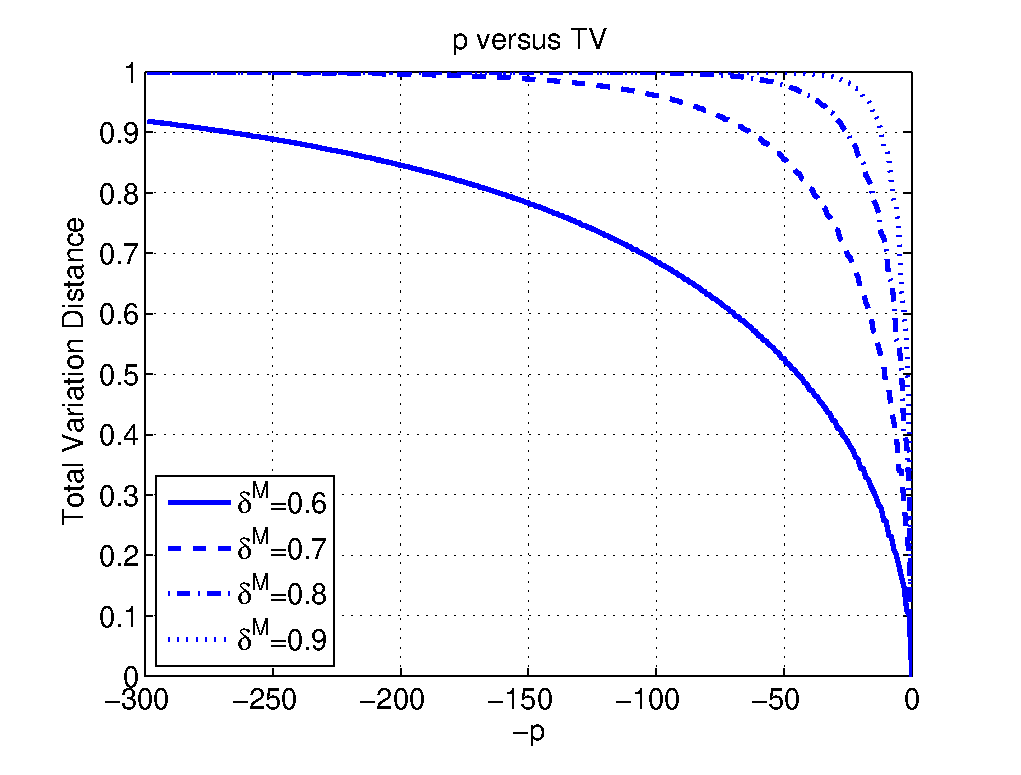
\includegraphics[width=0.5\textwidth]{deltaMexample1a}}
            {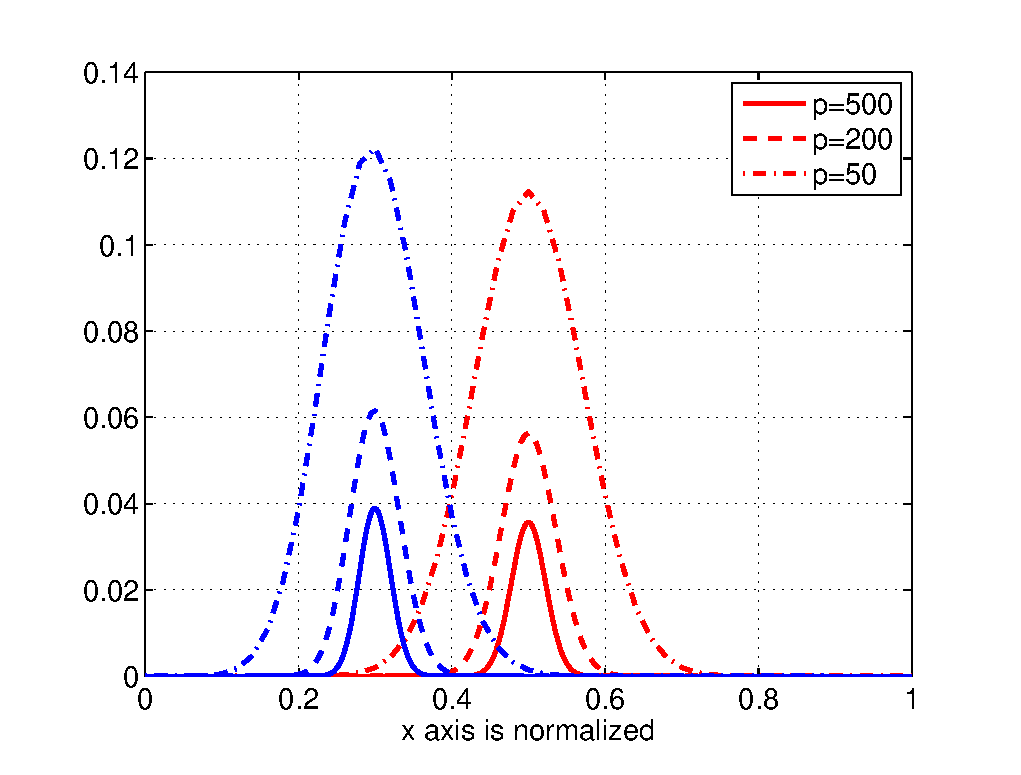
\includegraphics[width=0.5\textwidth]{deltaMexample1b}}}
\caption{\label{deltaMexample1}The left figure shows how one can evaluate
$|\omega^0-\bar{\omega}|_{TV}$, where $\omega^0$ has the form in equation (\ref{constantomega0}),
by finding the overlap area of two binomial distributions centered at $p\delta_\star^a$ and $p/2$.
When $p$ is large, the overlap area gets smaller. The right figure shows how
$|\omega^0-\bar{\omega}|_{TV}$ changes with $p$ for different $\delta_\star$'s. Since evolving
the distribution (\ref{constantomega0}) is equivalent to change $p$, this set of trajectories can
be also interpreted as $|\omega^k-\bar{\omega}|_{TV}$ for $k=300-p$}.
\end{figure}

\end{example}
From the above example, we can give the following theorem.
\begin{theorem}
For a $1$-D map $S:\Lambda \to \Lambda$ having symbolic dynamics, the family \\$(\Omega,\bar{\omega},(\omega^k_n)_{k=0,1,\ldots})_{n=1,2,\ldots}$ presents a total variation-cutoff in the relaxed sense, where
\begin{equation*} 
 \psi(\omega^0_n) =  \{.\underbrace{\delta_\star \delta_\star \cdots \delta_\star}_{n}\frac{1}{2}\frac{1}{2}\cdots\} 
\end{equation*}
for $\omega^0_n\in\bar{\Omega}$ and $0 \le \delta_\star \le 1$. 
\end{theorem}
\begin{proof}
Let $t_n = n$, when $k_n>(1+\epsilon)n$, $|\omega^k_n-\bar{\omega}|_{TV}=0$. When $k_n<(1-\epsilon)n$, $n-k_n>\epsilon n$, and 
\begin{align*}
      |\omega_n^{k_n}-\bar{\omega}|_{TV} &   = |\omega_n^{n-{(n-{k_n})}}-\bar{\omega}|_{TV} \\
                                         & \ge |\omega_n^{n-{\lceil\epsilon n \rceil}}-\bar{\omega}|_{TV}\\
                                         &   = |\omega_p^{{p-{\lceil\epsilon n \rceil}}}-\bar{\omega}|_{TV}  \text{ for any } p\ge n \\
                                         &\to 1 \text{ when } n \to \infty.
\end{align*}
\end{proof}

Theorem \ref{tentmapcutoff} is a special case of the above theorem with $\delta_\star = 1$. 



%%%%%%%%%%%%%%%%%%%%%%%%%%%%%%%%%%%%%%%%%%%%%%%%%%%%%%%%%%%%%%%%%%%%%%%%%%%%%%%%%%
\begin{example}
Suppose $\omega^0$ has stochastic symbol sequence as follows:
  \begin{eqnarray}
  \label{expw0}
   \psi(\omega^0) =  \{.\delta_0 \delta_1 \delta_2 \cdots\},
  \end{eqnarray}
where $\delta_i = \frac{1}{2} + \epsilon r^i$, $\epsilon \in [0,1/2]$ and $r\in [0,1]$. The reason we choose it to decay exponentially is that we can use the upper bound theorem with fixed $p$. Here the area under $\delta$ and above $\frac{1}{2}$ can be calculated by the sum of a geometric series. Let $(\delta^M_\star)^k = \delta_k$; then
  \begin{eqnarray}
   \frac{M_k}{2} = \frac{\delta_k}{1-r}.
  \end{eqnarray}
Hence choose $p = \lfloor \frac{1}{1-r} \rfloor $ for the upper bound theorem. $p$ is a constant so the analysis is easier (as we see in the previous example, $p$ affects the TV). We use the same $p$ for the lower bound theorem, so $(\delta^m_\star)^k = r^p(\delta_{k}-\frac{1}{2}) $. From the upper and lower bound theorems, the total variation distance to stationary at iteration $k$ can be bounded by
  \begin{eqnarray}
  \label{omegakbound}
    |\psi^{-1}((\delta^m)^k)-\bar{\omega}|_{TV} <|\omega^k-\bar{\omega}|_{TV}<|\psi^{-1}((\delta^M)^k)-\bar{\omega}|_{TV},
  \end{eqnarray}
where
  \begin{eqnarray}
  \label{defdeltamM}
   (\delta^m)^k = \{.\underbrace{(\delta^m_\star)^k (\delta^m_\star)^k \cdots (\delta^m_\star)^k}_{p}\frac{1}{2}\frac{1}{2}\cdots\}, \nonumber\\
   (\delta^M)^k = \{.\underbrace{(\delta^M_\star)^k (\delta^M_\star)^k \cdots (\delta^M_\star)^k}_{p}\frac{1}{2}\frac{1}{2}\cdots\}.
  \end{eqnarray}

\begin{figure}
\centerline{{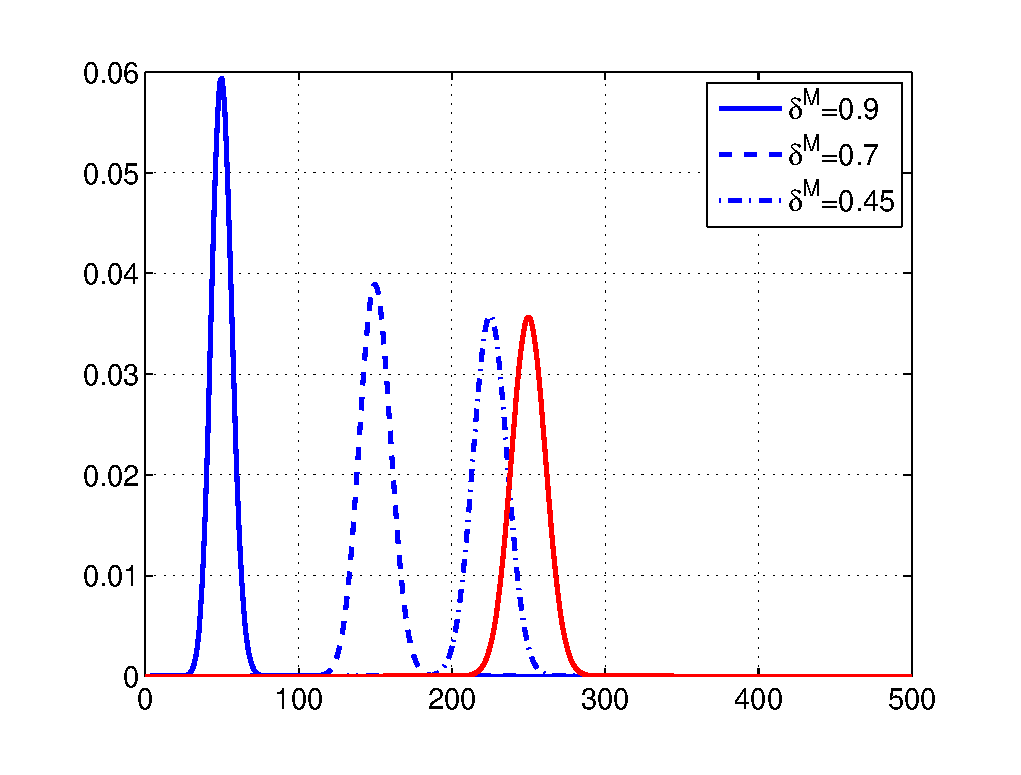
\includegraphics[width=0.5\textwidth]{deltaMexample2a}}
            {\includegraphics[width=0.5\textwidth]{deltaMexample2b}}}
\caption{\label{deltaMexample2}The left figure shows how one can evaluate the lower and upper
bounds of $|\omega^k-\bar{\omega}|_{TV}$, where $\omega^0$ has the form in equation (\ref{expw0}),
by finding the overlap area of two binomial distributions centered at
$p\delta_k=\frac{1}{2}+\epsilon r^k$ and $p/2$. In the right figure the upper bound and the lower
bound of $|\omega^k-\bar{\omega}|_{TV}$ by Theorems \ref{theoremub2} and \ref{theoremlb} are plotted,
as well as their approximations by Theorem \ref{theoremapproxlb}.}
\end{figure}
This is valid for each $k$. Similar to Example \ref{example:constantoega0}, we can plot the upper and lower bounds in a reduced space to see the movement of a binomial distribution. The left plot of Figure \ref{deltaMexample2} shows how the upper bound distribution moves toward the binomial distribution
centered at $p/2$ when $k$ increases, and then the TVs of upper bound and lower bound versus iteration plot is given
in the right plot of Figure \ref{deltaMexample2} for $\delta_0= 1$ and $r=0.998$.
Again, from the change of the overlap area of the left plot, it is not hard to understand how the concave shape is formed in the right plot.  

We need to stress here that to find the actual $|\omega^k-\bar{\omega}|_{TV}$ trajectory is impossible because one needs to evaluate (\ref{infiniteTV}) for each $\omega^k$. Even just to find an approximation of it using (\ref{finiteTV}), the computation cost is extremely large. This demonstrates the value of the upper and lower bound theorems. However, even so, we do not get much insight on how the bounds evolve because these two theorems give bounds based on the incomplete beta function. Hence here we would like to apply Theorem \ref{theoremapproxlb} regardless of its condition ($p \to \infty$ and $\delta_\star \to 1$). It should give us a pair of approximate upper and lower bounds,
\begin{eqnarray}
\label{expub}
|\omega^k -\bar{\omega}|_{TV}  &\stackrel{approx.}{\le}  &  \erf\left( \sqrt{\frac{p}{2}}\left((\delta_{\star}^M)^k-\frac{1}{2}\right)\right) \nonumber \\
                               & = &     \erf\left( \sqrt{\frac{1}{2(1-r)}} \epsilon^0r^k \right),
\end{eqnarray}
and
\begin{eqnarray}
\label{explb}
|\omega^k -\bar{\omega}|_{TV}  &\stackrel{approx.}{\ge} & \erf\left( \sqrt{\frac{1}{2(1-r)}} \epsilon^0 r^{\frac{1}{1-r}}r^k \right)  \nonumber \\
                               & = &  \erf\left( \sqrt{\frac{1}{2(1-r)}} \epsilon^0 e^{-1} r^k \right).
\end{eqnarray}
The approximated upper and lower bounds are plotted in the right of Figure \ref{deltaMexample2}, too. They are almost identical to the actual bounds.
Both (\ref{explb}) and (\ref{expub}) show the normal shapes, just like we see in example 1. Since
$(\delta_{\star}^M)^k-\frac{1}{2} = \epsilon^0 r^k$ decays exponentially (with factor $r$) to $0$, the trajectory
does not look like the error function itself. Instead, it has a sharper change before cutoff
happens and gets milder after it.
\end{example}
%%%%%%%%%%%%%%%%%%%%%%%%%%%%%%%%%%%%%%%%%%%%%%%%%%%%%%%%%%%%%%%%%%%%%%%%%%%%%%%%%%%%

The above two examples show the impact of $p$ and $\delta_{\star}^M$, which relate to the sum of
the stochastic symbol sequence and its largest entry. To summarize, the TV of the current distribution to the invariant distribution can be characterized by its upper and lower bounds, which correspond to $|\psi( (\delta^m)^k )^{-1}-\bar{\omega}|_{TV}$ and $|\psi( (\delta^M)^k )^{-1}-\bar{\omega}|_{TV}$. They
can be evaluated (and also approximated) and then the shape of $|\omega-\bar{\omega}|_{TV}$ is determined.
% which
%centered at $p\delta_{\star}^M$ (resp. $p\delta_{\star}^m$) and $p/2$. And so their TV can be bounded by $p$ and $\delta_{\star}^M$ (resp. $\delta_{\star}^m$). Isolating the
%change of $p$ or $\delta_{\star}^M$($\delta_{\star}^m$), the trajectory can be shown as the right
%plot of figure \ref{deltaMexample1} and the right plot of figure \ref{deltaMexample2}.



\subsection{Create cutoffs}
We have shown that an initial distribution like (\ref{expw0}) evolved by $P_S$ can have very similar $|\omega^k-\bar{\omega}|_{TV}$ trajectory to what one sees in a cutoff phenomenon. Now we want to take a further step to show that we can generate a set of initial disitributions $\omega_n$, which are a function of $n$, such that $\nu_n^k = |\omega_n^k-\bar{\omega}|_{TV}$ actually has the shape of (\ref{rdwalkshape}) when $n$ goes to infinity. We give the following theorem.
%%%%%%%%%%%%%%%%%%%%%%%%%%%%%%%%%%%%%%%%%%%%%%%%%%%%%%%%%%%%%%%%%%%%%%%%%%%%%%%%%%%%%
\begin{theorem}
Let $\omega_n^0 \in \bar{\Omega}$ have stochastic symbol sequence
 \begin{eqnarray}
    \psi(\omega^0_n) =  \{.\delta_0 \delta_1 \delta_2 \cdots\},
 \end{eqnarray}
where $\delta_i = \min\{\frac{1}{2}+\epsilon_n r_n^i,1\}$, and
 \begin{align}
 \begin{split}
          r_n &= e^{-\frac{2}{n}}.\\
          \epsilon_n &= \sqrt{\frac{n(1-r_n)}{4}},
 \end{split}
 \end{align}
The family $(\Omega,\bar{\omega},(\omega^k_n)_{k=0,1,\ldots})_{n=1,2,\ldots}$ presents a total variation-cutoff. In fact, 
Let $k = \frac{1}{4}n\log{n}+cn $; then for fixed $c\in \mathbb{R}$ as $n\to \infty$,
\begin{eqnarray}
\label{erfbound}
 %|\omega^k_n - \bar{\omega} |_{TV} \sim \erf \left(\frac{e^{-2c}}{\sqrt{8}}\right)
          \erf \left(\frac{e^{-2c-1}}{\sqrt{8}}\right)\le  |\omega^k_n - \bar{\omega} |_{TV} \le \erf \left(\frac{e^{-2c}}{\sqrt{8}}\right).
\end{eqnarray}
\end{theorem}

\begin{proof} From example 3, $|\omega^k_n - \bar{\omega}|_{TV}$ is bounded by (\ref{omegakbound}). When $n \to \infty$, $\epsilon_n$ goes to $\sqrt{\frac{1}{2}}$ and $r_n$ goes to $1$. Letting $k> \frac{-\log(2\epsilon_n)}{r_n}$ so that $\epsilon_n r_n^k<1/2$, and using the results of (\ref{expub}) and (\ref{explb}), we have
\begin{eqnarray}
                \erf\left( \sqrt{\frac{1}{2(1-r_n)}} \epsilon_n e^{-1} r_n^k \right)
            \le |\omega^k_n - \bar{\omega}|_{TV}
            \le \erf\left( \sqrt{\frac{1}{2(1-r_n)}} \epsilon_nr_n^k \right).
\end{eqnarray}
Now these bounds are not approximations because the conditions of Theorem \ref{theoremapproxlb} are satisfied. 
Substituting the expresstion $\epsilon_n$ and $r_n$ into above inequality gives
\begin{eqnarray}
                \erf\left(\sqrt{\frac{n}{8}}e^{-\frac{2k}{n}-1}  \right)
            \le |\omega^k_n - \bar{\omega}|_{TV}
            \le  \erf\left(\sqrt{\frac{n}{8}}e^{-\frac{2k}{n}}  \right),
\end{eqnarray}
%Thus we have
%\begin{eqnarray}
  %     |\omega^k_n - \bar{\omega} |_{TV} \sim \erf\left(\sqrt{\frac{n}{8}}e^{-\frac{2k}{n}}  \right)
%\end{eqnarray}
Letting $k = \frac{1}{4}n\log{n}+cn $ for $c\in \mathbb{R}$, and substituting into the above expression, we get the desired result (\ref{erfbound}), and hence it presents a cutoff.
\end{proof}

%%%%%%%%%%%%%%%%%%%%%%%%%%%%%%%%%%%%%%%%%%%%%%%%%%%%%%%%%%%%%%%%%%%%%%%%%%%%%%%%%%%%%%

The key idea of the above theorem is that we know for a pair of $(\epsilon,r)$, the stochastic symbol sequence with $\delta_i = \frac{1}{2}+\epsilon r^i$ has a normal shape cutoff. Hence we equate the coefficients to find $(\epsilon_n,r_n)$ as functions of $n$ that have the same $|\omega^k_n - \bar{\omega} |_{TV}$ as the random walk on a $n$-dimensional hypercube problem. In this case the $\epsilon_n$ we find is larger than $1/2$ when $n>1$, which is prohibited in the stochastic symbol sequence ($\delta_0>1$). However, we set $\delta^i=1$ for $i<\frac{-\log(2\epsilon_n)}{r_n}$ and then when $k> \frac{-\log(2\epsilon_n)}{r_n}$, the remaining sequence is exponential and Theorem \ref{theoremapproxlb} is applicable again.

Following the same rule, we can reproduce any cutoff with normal shape in relaxed sense by a family $\{\Omega,\bar{\omega},(\omega_n^k)_{k=0,1,\ldots}\}_{n=0,1,\ldots}$, where $\omega_n^{k+1} = P_S(\omega_n^k)$, and $P_S$ is the Perron-Frobenius of map $S:\Lambda \to \Lambda$, which has symbolic dynamics.


%%%%%%%%%%%%%%%%%%%%%%%%%%%%%%%%%%%%%%%%%%%%%%%%
\subsection{What causes cutoffs?}
%%%%%%%%%%%%%%%%%%%%%%%%%%%%%%%%%%%%%%%%%%%%%%%%
As we have mentioned before, the analysis and proof of cutoffs are usually very hard, but to understand what causes cutoffs can be quite easy and we discuss it here to further explain the relation between the cutoff of finite Markov Chains and chaotic map mixing. Let us focus on the total variation-cutoff with normal shape. We claim that if the process is composed of many (almost) independent small processes, then it has the key factor to present a cutoff. To explain this, again we use the random walk on an $n$-dimensional hypercube as the example. Let $I=\{0,1\}$; the coordinate of the particle can be represented as a vector in $I^n$. For instance, the point starting at the origin is
\begin{eqnarray*}
 x^0 = (0,0,\ldots,0).
\end{eqnarray*}
Each of the coordinates equals zero with probability $1$. At each iteration, the particle can stay fixed or choose one of the coordinates randomly. For this chosen coordinate, if it is $0$, it becomes $1$ and vice versa. Under this big process with $n$ coordinates and $2^n$ states, we can discuss $n$ much smaller random processes: the value of each coordinate. All of these small processes are not independent of each other. For example, at iteration $1$, suppose we know that the first coordinate is $1$; then we immediately know all of the other coordinates are zeros. 
So even though all of these small processes are identical and easy to analyze, to calculate the probability of the $2^n$ states by the joint probability of the small processes is still not possible. Nonetheless, a very important fact is: they become almost independent after just several iterations. This is also easy to imagine: suppose $n = 1000$ and $k = 10$; knowing that the first coordinate is $1$ is almost not helpful to know the value of any other coordinates. The tendency that these small processes have to become independent of each other is so strong that even if we just assume they are independent in the beginning, and calculate $\omega_n^k$ by the joint probability of these independent small processes, we get a very good approximation of the actual process. This simplification corresponds to the continuous-time random walk on a hypercube problem \cite{Diaconis1990}. The analysis of this problem is much easier than the original problem and it presents the same cutoff. Therefore, we can conclude that even if the original process is very complicated, the almost independence of the small processes is the key for the whole process to present a cutoff. 

Then how does this almost independence fit into the chaotic map evolution? Remember that the probability space we discuss is $\bar{\Omega}$, and from Lemma \ref{lemma:independency}, when a point $x$ with probability distribution $\omega \in \bar{\Omega}$ is evolved by the chaotic map with symbolic dynamics, $\phi(x^k)_i$ and $\phi(x^k)_j$ are independent of each other for all $k$ and $i\neq j$. So this process looks like it is composed of an infinite number of independent small processes. Thus we can design the exponential type stochastic symbol sequence to make all these small processes behave like the process we see in one coordinate of the hypercube and achieve similar TV trajectories. It is purely the special property of $\omega \in \bar{\Omega}$ for chaotic maps with symbolic dynamics that makes this possible. This clearly explains why we observe cutoffs in chaotic map evolution.  

 

%%%%%%%%%%%%%%%%%%%%%%%%%%%%%%%%%%%%%%%%%%%%%%%%
%\subsection{When $\omega \notin \bar{\Omega}$}
%%%%%%%%%%%%%%%%%%%%%%%%%%%%%%%%%%%%%%%%%%%%%%%%

%The above results are only applicable when $\omega \in \bar{\Omega}$, and is quite restrictive. An easy extension can be made for all $\omega \in \Omega$ and are ``close'' to $\bar{\Omega}$ in total variation distance. Given $\omega^0 \in \Omega $, suppose we can find an $\tilde{\omega}^0\in \bar{\Omega} $ such that $|\omega^0- \tilde{\omega}^0|_{TV}$ is small, then use triangular inequality, for any $k \ge 0$
%\begin{eqnarray}
%     \left| |\tilde{\omega}^k-\bar{\omega} |_{TV}  -  |\omega^k-\tilde{\omega}^k|_{TV}\right|
%     \le |\omega^k-\bar{\omega}|_{TV}
%     \le |\tilde{\omega}^k-\bar{\omega}|_{TV} + |\omega^k-\tilde{\omega}^k|_{TV}
%\end{eqnarray}
%Total variation distance is non-increasing, thus $|\omega^k-\tilde{\omega}^k|_{TV} \le |\omega^0-\tilde{\omega}^0|_{TV} $. Let the upper and lower bounds obtained by theorem \ref{theoremub} and \ref{theoremlb} for $|\tilde{\omega}^k-\bar{\omega} |_{TV}$ be $b_l^k$ and $b_u^k$, and let $|\omega^0-\tilde{\omega}^0|_{TV} = b^0$, we have
%\begin{eqnarray}
%     |b_l^k-b^0| \le |\omega^k-\bar{\omega}|_{TV}  \le b_u^k+b^0
%\end{eqnarray}
%How do we find $\tilde{\omega}^0$ such that $|\omega^0- \tilde{\omega}^0|_{TV}$ is minimized so that the bound is tighter? The easiest way is letting $\tilde{\omega}^0 = \psi(\omega^0) $. This may not be the best fitting of $\omega^0$, however, it is believed that if $\psi(\omega^0)$ is not a good fitting of $\omega^0$, there is not much space to improved by finding another $\tilde{\omega}^0$. Again, we want to stress that the upper and lower bounds are not practically useful, but they do characterize the behavior of the convergence trajectory for a set of $\omega^0$.



%%%%%%%%%%%%%%%%%%%%%%%%%%%%%%%%%%%%%%%%%%%%%%%%%%%%%%%%%%
%%%%%%%%%%%%%%%%%%%%%%%%%%%%%%%%%%%%%%%%%%%%%%%%%%%%%%%%%%
%\chapter{Conclusion}
%%
%  Thesis Conclusion
%
Here is my thesis conclusion




% and the end material

\appendix

%\include{appendix1}
%\include{appendix2}
%\include{appendix3}



%\include{bibliography}

\nocite{*}


    %\bibliographystyle{plain}
     \bibliographystyle{abbrv}
    \bibliography{../bib/mixingbib}


\end{document}

